%%%%%%%%%%%%%%%%%%%%%%%%%%%%%%%%%%%%%%%%%
% RRI template for TechDocs
%
% Original author:
% Juan Tomas Sayago
%

% Instructions for using this template:
% This title page compiles as is. If you wish to include this title page in 
% another document, you will need to copy everything before 
% \begin{document} into the preamble of your document. The title page is
% then included using \titleAT within your document.
%
%%%%%%%%%%%%%%%%%%%%%%%%%%%%%%%%%%%%%%%%%

%----------------------------------------------------------------------------------------
%	PACKAGES AND OTHER DOCUMENT CONFIGURATIONS
%----------------------------------------------------------------------------------------
%extsizes support 8pt to 20pt
\documentclass[12pt]{extreport}		
\usepackage{amsmath,amsthm}
\usepackage{amssymb}
\usepackage[english]{babel}
\usepackage{latexsym}
\usepackage{amsfonts}
\usepackage{graphicx}
\usepackage{float}
\usepackage{graphics}
\usepackage{epsfig}
\usepackage[T1]{fontenc}
\usepackage[utf8]{inputenc}
\usepackage[hyperfootnotes=false]{hyperref}
\usepackage{authblk}
%\usepackage[]{mcode}
\usepackage[paper=a4paper,top=25mm,bottom=25mm,right=25mm, left=25mm]{geometry}
\usepackage{xcolor} 
\usepackage{tocbibind}
\usepackage{multicol}
\usepackage{tabto}
\usepackage[numbers]{natbib}
\usepackage[symbol]{footmisc}
\usepackage[toc,page]{appendix}
\usepackage{enumitem}
\usepackage{listings}
\usepackage{lstautogobble}
\usepackage[export]{adjustbox}[2011/08/13]
\usepackage{subcaption}
\usepackage{booktabs}
\usepackage{fancyvrb}
\usepackage{forest}
\usepackage{pdfpages}
\usepackage{acronym}
\usepackage{titlesec}
%\usepackage{sectsty,lmodern}
\usepackage{titletoc}
%\usepackage{txfonts}
%Times New Romans Font
\usepackage{tgtermes}

%Set size of chapter title, section title, subsection title
\newcommand{\chapfnt}{\fontsize{16bp}{19}\selectfont}
\newcommand{\secfnt}{\fontsize{14bp}{14}\selectfont}
\newcommand{\ssecfnt}{\fontsize{12bp}{14}\selectfont}
\titleformat{\chapter}[hang]
{\vspace{-2.75cm}\centering\chapfnt\bfseries}{\MakeUppercase\chaptertitlename\ \thechapter:}{20pt}{\MakeUppercase}[{\vspace{0.5cm}\titlerule[1.75pt]\vspace{-0.2cm}}]

%\titleformat{\chapter}[hang] 
%{\vspace{-2.25cm}\centering\huge\bfseries{\MakeUppercase\chaptertitlename\ \thechapter:}{16pt}{\MakeUppercase}[{\titlerule[0.8pt]\vspace{-1cm}}]

\titleformat{\section}
{\normalfont\secfnt\bfseries}{\thesection}{1em}{}

\titleformat{\subsection}
{\normalfont\ssecfnt\bfseries}{\thesubsection}{1em}{}

\titlespacing*{\chapter} {0pt}{50pt}{40pt}
\titlespacing*{\section} {0pt}{3.5ex plus 1ex minus .2ex}{2.3ex plus .2ex}
\titlespacing*{\subsection} {0pt}{3.25ex plus 1ex minus .2ex}{1.5ex plus .2ex}

\AtBeginDocument{\renewcommand{\bibname}{References}}

\numberwithin{figure}{chapter}
\numberwithin{table}{chapter}
\lstset{basicstyle=\ttfamily,
  mathescape=true,
  escapeinside=||,
  autogobble}

\titlecontents{chapter}% <section-type>
  [0pt]% <left>
  {\bfseries}% <above-code>
  {\chaptername\ \thecontentslabel:\quad}% <numbered-entry-format>
  {}% <numberless-entry-format>
  {\hfill\contentspage}% <filler-page-format>



\newcommand*{\Doctitle}{Document Title} % Generic publisher logo
\newcommand*{\Docstitle}{Document subtitle} % Generic publisher logo
\renewcommand{\thefootnote}{\fnsymbol{footnote}}
\title{\Doctitle} % Article title

\date{}

\newcommand*{\plogo}{Number} % Generic publisher logo
\newcommand*{\keywords}{Regional economics; R1} % Generic publisher logo

\renewenvironment{itemize}{
  \begin{list}{}{
    \setlength{\leftmargin}{-1em}
  }
}{
  \end{list}
}

\definecolor{wvublue}{HTML}{003366}
\definecolor{wvugold}{HTML}{FFCC00}

\newlist{steps}{enumerate}{1}
\setlist[steps, 1]{label = Step \arabic*:}

%----------------------------------------------------------------------------------------------------


% ---------------------------------------------------------------------
\RequirePackage{fancyhdr}  % Needed to define custom headers/footers
\RequirePackage{lastpage}  % Number of pages in the document
\pagestyle{fancy}          % Enables the custom headers/footers
% Headers
\lhead{}%
\chead{}%
\rhead{} %
% Footers
\lfoot{}%
\cfoot{\thepage}%
\rfoot{}%
\renewcommand{\headrulewidth}{0pt}% % No header rule
\renewcommand{\footrulewidth}{0pt}% % No footer rule
% ---------------------------------------------------------------------



%----------------------------------------------------------------------------------------
%	TITLE PAGE
%----------------------------------------------------------------------------------------
\newcommand*{\titleRRITD}{\begingroup % Create the command for including the title page in the document
\thispagestyle{empty}
\centering % Center all text
{\vspace{-2.75cm}\chapfnt\MakeUppercase{\textbf{CrazyOS: A Real Mode Operating System for\\[0.25\baselineskip]Educational Purposes}}}\\[1.0\baselineskip]
{\textbf{MAJOR PROJECT REPORT\\[1.0\baselineskip]\textit{Submitted in partial fulfilment of the requirements for the award of the degree\\[0.5\baselineskip]of}}}\\[0.5\baselineskip]
{\secfnt \textbf{\MakeUppercase{Bachelor of Technology}\\[0.5\baselineskip]\textit{\normalsize in}\\[0.5\baselineskip]\secfnt\MakeUppercase{Electrical \& Electronics Engineering}}}\\[0.5\baselineskip]
{\textbf{\textit{\normalsize by}}}\\[0.5\baselineskip]
\begin{multicols}{4}
{\normalsize
\centering{
\textbf{Praneet Kapoor}\\
\textbf{04115604918}\\
\textbf{Rachit Jain}\\
\textbf{04315604918}\\
\textbf{Shristi Sharma}\\
\textbf{05415604918}\\
%\columnbreak
\textbf{Sumit Gaur}\\
\textbf{06115604918}\\}
}
\end{multicols}
{\normalsize \textbf{\textit{Under the guidance\\of\\{Mr. Md. Saquib Faraz\\Assistant Professor}}}}
%EEE department
%%%%%%%%%%%%%%%%%%%%%%%%%%%%%%%%%%%%%%%%%%%%%%%%%%%%%%%%%%%%%%%
\vspace{0.5cm}
\begin{figure}[h]
\centering
\protect
\includegraphics[scale=1.5]{figures/logo-adgitm.eps}
\end{figure}
\vspace{0.5cm} % Whitespace between the title and short horizontal line
%%%%%%%%%%%%%%%%%%%%%%%%%%%%%%%%%%%%%%%%%%%%%%%%%%%%%%%%%%%%%%%
\begin{center}
\makebox[\textwidth][c]{\MakeUppercase{\textbf{Department of Electrical \& Electronics Engineering}}}
\newline
\makebox[\textwidth][c]{\MakeUppercase{\textbf{Dr. Akhilesh Das Gupta Institute of Technology and Management}}}
\newline
\makebox[\textwidth][c]{\MakeUppercase{\textbf{(Affliated to Guru Gobind Singh Indraprastha University, Delhi)}}}
\newline
\makebox[\textwidth][c]{\MakeUppercase{\textbf{New Delhi - 110053}}}
\newline
\makebox[\textwidth][c]{\MakeUppercase{\textbf{June 2022}}}
\end{center}
\vfill % Whitespace between the author name and publisher text
\endgroup}

%----------------------------------------------------------------------------------------
%	BLANK DOCUMENT
%----------------------------------------------------------------------------------------
\begin{document}

%%%%%%%%%%%%%%%%%%%%%%%%%%%%%%%%%%%%%%%%
%Adjust this to fix line spacing!!
\linespread{1.25}\selectfont
%%%%%%%%%%%%%%%%%%%%%%%%%%%%%%%%%%%%%%%%

\titleRRITD
%%%%%%%%%%%%%%%%%%%%%%%%%%%%%%%%%%%%%%%%%%%%%%%%%%%%%%%%%%%%%%%%%%
\newpage
\pagenumbering{roman}
\linespread{1.5}\selectfont
\chapter*{\centering{CANDIDATES' DECLARATION}}
\addcontentsline{toc}{chapter}{CANDIDATE'S DECLARATION}
It is hereby certified that the work which is being presented in the B.Tech Major Project Report entitled \textbf{CrazyOS: A Real Mode Operating System for Educational Purposes} in partial fulfilment of the requirements for the award of the degree of \textbf{Bachelor of Technology} and submitted in the \textbf{Department of Electrical \& Electronics Engineering} of \textbf{Dr. Akhilesh Das Gupta Institute of Technology \& Management, New Delhi (Affiliated to Guru Gobind Singh Indraprastha University, Delhi)} is an authentic record of our own work carried out during the period from \textbf{February 2022 to June 2022} under the guidance of \textbf{Mr. Md. Saquib Faraz, Assistant Professor, EEE department}.\\[1.0\baselineskip]
The matter presented in the B. Tech Major Project Report has not been submitted by us for the award of any other degree of this or any other Institute.\\[\baselineskip]
\begin{multicols}{4}
{\normalsize
\centering{
\textbf{Praneet Kapoor}\\
\textbf{04115604918}\\
\textbf{Rachit Jain}\\
\textbf{04315604918}\\
\textbf{Shristi Sharma}\\
\textbf{05415604918}\\
%\columnbreak
\textbf{Sumit Gaur}\\
\textbf{06115604918}\\}
}
\end{multicols}
This is to certify that the above statement made by the candidates is correct to the best of our knowledge.\\[\baselineskip]
\begin{multicols}{2}
\centering
{\hspace{-2.5cm}
\textbf{Mr. Md. Saquib Faraz}\\
\hspace{-2.5cm}
\textbf{Assistant Professor}\\
\columnbreak
\centering\textbf{\hspace{2.5cm}Mr. Ajit Kumar Sharma\\\hspace{2.5cm}H.O.D., EEE Deptt.}\\
}
\end{multicols}
The B. Tech. Major Project Viva-Voice Examination of Praneet Kapoor, Rachit Jain, Shristi Sharma, and Sumit Gaur has been held on\\[\baselineskip]
\begin{multicols}{2}
\centering\textbf{\hspace{-2.5cm}Dr. Amruta Pattnaik\\\hspace{-2.5cm}Project Coordinator}\\
\columnbreak
\centering\textbf{\hspace{1cm}(Signature of the External Examiner)}\\
\end{multicols}


%%%%%%%%%%%%%%%%%%%%%%%%%%%%%%%%%%%%%%%%%%%%%%%%%%%%%%%%%%%%%%%%%%
\newpage
\chapter*{\centering Abstract}
\addcontentsline{toc}{chapter}{ABSTRACT}
Technical education of undergraduate students should ensure that they are provided with practical knowledge which makes them fit for the ever changing industry. One of the ways of accomplishing this is by attempting to include project based learning alongside regular coursework. This project is a step towards this direction. We have presented a single-user, single-tasking, real mode operating system. The operating system comes with two applications, a shell and a line editor. A library of subroutines has also been created which includes custom implementation of getchar, putchar, printf, strlen, strcmp, strcpy and atoi in x86 assembly language. With only 1690 lines of code, the source code of the operating system can be easily understood by students and then used as a sandbox for learning about the design of the 8086 microprocessor and the original IBM PC.

%%%%%%%%%%%%%%%%%%%%%%%%%%%%%%%%%%%%%%%%%%%%%%%%%%%%%%%%%%%%%%%%%%
\newpage
\chapter*{\centering Acknowledgements}
\addcontentsline{toc}{chapter}{ACKNOWLEDGEMENTS}
We express our deep gratitude to \textbf{Mr. Md. Saquib Faraz, Assistant Professor, Department of Electrical \& Electronics Engineering} for his valuable guidance and suggestions throughout our project work.\\
We would like to extend our sincere thanks to \textbf{Mr. Ajit Kumar Sharma, Head of the Department, EEE} for his time to time suggestions to complete our project work. We are also thankful to \textbf{Prof. (Dr.) Sanjay Kumar, Director} for providing us the facilities to carry out our project work.\\
We are thankful to  \textbf{Dr. Amruta Pattnaik, Project Coordinator} for her valuable guidance.\\[2.5\baselineskip]
\begin{multicols}{4}
{\normalsize
\centering{
\textbf{Praneet Kapoor}\\
\textbf{04115604918}\\
\textbf{Rachit Jain}\\
\textbf{04315604918}\\
\textbf{Shristi Sharma}\\
\textbf{05415604918}\\
%\columnbreak
\textbf{Sumit Gaur}\\
\textbf{06115604918}\\}
}
\end{multicols}
%%%%%%%%%%%%%%%%%%%%%%%%%%%%%%%%%%%%%%%%%%%%%%%%%%%%%%%%%%%%%%%%%%
\renewcommand*\contentsname{TABLE OF CONTENTS}
\renewcommand*\listfigurename{LIST OF FIGURES} 
\renewcommand*\listtablename{LIST OF TABLES} 
\thispagestyle{empty}
\newpage
\tableofcontents
\newpage
\listoffigures
\newpage
\listoftables

\newpage
\chapter*{List of Abbreviations}
\addcontentsline{toc}{chapter}{LIST OF ABBREVIATIONS}
\begin{acronym}
\acro{ACPI}{Advanced Configuration and Power Interface}
\acro{AGC}{Apollo Guidance Computer}
\acro{AICTE}{All India Council for Technical Education}
\acro{ANSI}{American National Standards Institute}
\acro{APM}{Advanced Power Management}
\acro{ARM}{Advanced RISC Machines, originally Acorn RISC Machine}
\acro{BDA}{BIOS Data Area}
\acro{BIOS}{Basic Input/Output System}
\acro{BIU}{Bus Interface Unit}
\acro{CHS}{Cylinder-Head-Sector}
\acro{CP/M}{Control Program/Monitor, later Control Program for Microcomputers}
\acro{CPU}{Central Processing Unit}
\acro{CTSS}{Compatible Time Sharing System}
\acro{DEC}{Digital Equipment Corporation}
\acro{DIP}{Dual Inline Package}
\acro{DOS}{Disk Operating System}
\acro{EBDA}{Extra BIOS Data Area}
\acro{EDSAC}{Electronic Delay Storage Automatic Calculator}
\acro{EDVAC}{Electronic Discrete Variable Automatic Computer}
\acro{ENIAC}{Electronic Numerical Integrator and Comparator}
\acro{EU}{Execution Unit}
\acro{FAT}{File Allocation Table}
\acro{GCC}{GNU Compiler Collection}
\acro{GNU}{GNU is Not UNIX}
\acro{IBM}{International Business Machines}
\acro{IC}{Integrated Circuit}
\acro{IT}{Information Technology}
\acro{IVT}{Interrupt Vector Table}
\acro{LCD}{Liquid Crystal Display}
\acro{LMA}{Low Memory Area}
\acro{MBR}{Master Boot Record}
\acro{MINIX}{Mini-UNIX}
\acro{MIT}{Massachusetts Institute of Technology}
\acro{MULTICS}{MULTiplexed Information and Computation Service}
\acro{NASA}{National Aeronautics and Space Administration}
\acro{NASM}{Netwide ASseMbler}
\acro{OEM}{Original Equipment Manufacturer}
\acro{OS}{Operating System}
\acro{PC}{Personal Computer}
\acro{PCI}{Peripheral Component Interconnect}
\acro{PDP}{Programmed Data Processor}
\acro{PIC}{Programmable Interrupt Controller}
\acro{PIT}{Programmable Interval Timer}
\acro{RAM}{Random-Access Memory}
\acro{RISC}{Reduced Instruction Set Computer}
\acro{ROM}{Read-Only Memory}
\acro{UEFI}{Unified Extensible Firmware Interface}
\acro{UMA}{Upper Memory Area}
\acro{UNIVAC}{Universal Automatic Computer}
\end{acronym}
%%%%%%%%%%%%%%%%%%%%%%%%%%%%%%%%%%%%%%%%%%%%%%%%%%%%%%%%%%%%%%%%%%
\newpage
\pagenumbering{arabic}
\linespread{1.5}\selectfont
\chapter{\centering Introduction}
\section{Introduction}
Digital electronics and programming has become the backbone of every industry. To undermine the value of digital computers and programming skills in 21st century would be an indication of the ignorance of the person making this judgement. Therefore, it becomes highly important that all undergrad students of engineering and various other technical discipline have 
\begin{enumerate}
   \item at least a rudimentary knowledge of computer hardware, and 
   \item basic programming skills in a high level language, preferably Python 3.
\end{enumerate}
The depth of such knowledge would depend upon the profession they wish to undertake.\\
For an electrical engineer, having an understanding of underlying hardware of a computer is of utmost importance. With the mathematical training they have along with their knowledge of electronics, electrical engineers are the ones who are responsible for designing the next generation computers and programming languages. This has been true in the history of computing. ENIAC, IBM 1401, Apollo Guidance Computer (AGC), Apple II, the original IBM PC, and many other similar revolutionary computers were all designed by electrical engineers. C programming language and UNIX operating system, both of which have been the backbone of the industry for over 50 years, were developed by Ken Thompson and Dennis Ritchie, both of whom were electrical engineers. The development of Linux by Linus Torvalds was also motivated by his curiosity to understand the underlying hardware of his new i386 IBM PC \cite{torvalds2001just}. TempleOS, a 64-bit ring 0 operating system was designed from scratch by Terry Davis, an electrical engineer, in spirit of the Commodore VIC-20 he used in his youth \cite{kyrou2017art}. This makes it clear that electrical engineers also enrich the field of computer architecture and programming by their contributions. A similar case can be made for other fields like mathematics and physics. Therefore, the widely held belief that programming is for those in the field of computer science or information technology (IT) is wide off the mark.\\
Now, engineering is a practical profession. A good engineer should be able to use fundamental principles to solve problems or derive practical results. The ability to do so requires experience, which is often termed as "\textit{getting hands dirty}". It is of primary importance that an engineering student should have their hands sufficiently dirty in the profession they wish to pursue. A student interested in pursuing a career in silicon industry should have considerable experience in designing systems on an FPGA board. If he\footnote[1]{"He" should be read as "he or she" throughout the report.} has only memorized the important principles from some standard book, that student will have no value in the industry. This is similar to studying mathematics: learning theory is not enough, one needs to solve enough examples to get a \textit{feel} for the concept at hand. It is also possible that while getting their hands dirty in a field they disliked at first, they might find it likeable.\\
It were these opportunities to develop practical experience which were found to be missing from the course on Microprocessers and Microcontrollers. The course, in a span of 4 units and 45 hours, covers 8085 and 8086 microcontrollers, their support components (8259 PIC, 8289 bus arbiter, LCD, stepper motor, etc.), and 8051 microcontroller. Instead of following texts like \textit{The 8086 Family User's Manual} \cite{intel1979the}, students and teachers alike follow notes and presentations which don't talk about the practical side of various concepts like segmentation, effective address calculation and string operations, to name a few. Lab experiments consist of writing code to multiply and divide two numbers, move strings from one location to another, and control a stepper motor. Rare and costly development kits, and toy emulators like emu8086 are used in favour of professional tools like NASM and QEMU. In the end, students treat it like another boring subject with "\textit{no possible application in the future}".\\
Disgruntled by the approach taken in teaching one of his favourite subjects, one of the authors of this report (Kapoor), decided to write his own 16-bit operating system from scratch. He considered this to be fun challenge which would allow him to tinker with the hardware and understand the architecture of 8086 microprocessor and the original IBM PC. His objective at first was to develop a UNIX like operating system. However, as UNIX and its derivatives (Linux, MINIX, BSD, etc.) are complex systems and developing them would require ample amount of free time, it was decided that operating system designed would be a simple one consisting of just a primitive shell and line editor. Basic commands can be executed from shell. Students can develop the their own programs using the libraries provided by the author, assemble using NASM, create a virtual disk and run it in real mode on QEMU's emulation of i386 based IBM PC. Various unconventional decisions were made while making this operating system, some of which were:
\begin{enumerate}
\item Several standard functions like \verb|printf|, and \verb|strcmp| were written from scratch following some simple non-standard calling conventions.
\item Instead of using object files and a linker to produce the final binary of the operating system, source files are combined with each other using \verb|%include| preprocessor directive. Source files are prevented from getting included more than once by using the \verb|%ifndef %define| \verb|%endif| guard (which is also used in C) \cite{nasm2015doc}.
\item Filesystem of the operating system is extremely simple. Files are stored in contiguous sectors and are terminated with a magic number, \verb|0xaa|. If the user has not kept a track of the sectors belonging to a particular file, he will most probably overwrite a file during disk write operation. There is no concept of directories.   
\end{enumerate}
Due to such unusual design of the operating system, it was named \textit{CrazyOS} by its creator.
CrazyOS is a single-user, single-tasking real mode operating system which, along with its bootloader, is written in x86 assembly language from scratch. It features a shell and a line editor. Being just 1690 lines of code, students can use it as a sandbox to gain a practical understanding of the 8086 microprocessor and architecture of the IBM PC.

\section{Literature Survey}
The purpose of this literature survey is to provide the reader with a frame of reference from which they can understand the motivation, design choices, and the overall scope of this project. We begin with informal definitions of several key concepts which will be encountered in this report. A brief history of computing systems, and the design of the 8086 microprocessor and the original IBM PC are discussed. We conclude this literature survey with a brief discussion of the deficiencies of the current engineering and technical education in India.

\subsection{Algorithms and Programs}
The definition of computer has gone a several changes throughout history. Before 1950's, the term usually referred to a person who had the job to do calculations or \textit{computations} \cite{evans2020broad}. Nowadays, it refers to a machine which processes data according to instructions fed into it. Majority of such machines are made out of electronic components and work on the principles of digital logic. Therefore, by the term computer one implicitly refers to a \textit{digital electronic computing system} \cite{ionescu2015categories}.  One common denominator throughout this transformation of computing systems has been that they need to be told to perform a particular task. The task to be performed is usually divided into smaller, manageable tasks or instructions. A sequence of such tasks is called an \textit{algorithm}. Each sub-task which makes up an algorithm is called a \textit{step} or an \textit{instruction}. Algorithms are usually written in a human language or mathematical symbols or, in general, both.\\
A good algorithm has five important features \cite{knuth1997art}:
\begin{enumerate}
\item \textit{Finiteness}: It must stop after a finite number of steps.
\item \textit{Definiteness}: Each step of the algorithm must be precisely defined.
\item \textit{Input}: An algorithm should have zero or more inputs.
\item \textit{Output}: An algorithm should have one or more outputs.
\item \textit{Effectiveness}: An algorithm is said to be effective if, in principle, if each of its steps can be executed manually, using pencil and paper, in a finite length of time.
\end{enumerate}
A simple example at this point would be helpful. Consider a student who is given the task to print out whether a given number is prime or not. He will first begin by defining prime numbers.\\
\textbf{Definition:} A number is said to be prime if it is only divisible by 1 and the number itself.\\
With this definition at hand, it becomes obvious that to test whether a number $N$ is prime or not, we have to check whether it is divisible by any other natural number except for 1 and itself. Upon inspection the student might observe that one does not need to test $N$'s divisibility with numbers greater than $N / 2$. The final algorithm that is obtained is:
\begin{steps}[leftmargin=2cm]
\item $n = 2$, $N = 0$.
\item Input $N$.
\item If $n > N/2$, then jump to step 6. 
\item If $N$ is divisible by $n$, then jump to step 7.
\item If $N$ is not divisible $n$, then $n = n + 1$ and jump to step 3.
\item Print \verb|N is a prime number| and end program.
\item Print \verb|N is not a prime number| and end program.
\end{steps}
A modern digital computer would not be able to understand these commands. It can only understand and execute instructions native to its architecture. A program consisting of opcodes of instructions and data, all in binary/hexadecimal format, is called \textit{machine code}. A file consisting of machine code is called a \textit{binary file} or, simply, \textit{binary}. A computer is able to understand only binaries and executes them in one shot (provided they mean something. Not every hexadecimal number can be mapped to an opcode). However, implementing any algorithm in machine code would take a significant amount of time. Debugging the binary would be even more troublesome. 
The problem can be solved by defining a language which satisfies the following criteria:
\begin{enumerate}
\item After sufficient training, a human being should be able to implement and debug algorithms in this language.
\item The algorithm implemented in this language can be easily converted into a binary using some conversion tool.
\end{enumerate}
A language satisfying both of these criteria is called a \textit{programming language}. The act of writing code in a programming language is called \textit{programming} or \textit{coding}. An algorithm implemented in such a language is called a \textit{program} or \textit{code}.\\
The simplest kind programming language is \textit{assembly language} (One can call machine code as a programming language, however, it is no longer used directly to practically program any computer). In assembly language, every instruction and register, instead of being referred by their opcode, are referred by a mnemonic. Labels are used to mark locations instead of hardcoded addresses. An \textit{assembler} is used to convert these mnemonics and labels into machine code.\\
While learning assembly language is not impossible, it has, however, a very steep learning curve. This calls the need for \textit{higher level languages} (HLL). These programming languages mask the programmer from the architecture of the machine they are working on. This enables them to direct their energies towards developing and implementing algorithm to get the task done. Every HLLs have its own set of symbols for defining operations and data structures, and semantics and syntax for successfully implementing algorithms \cite{hthreads2006glossary}\cite{chu1975concepts}. C is one such programming language. The algorithm for testing whether a number is prime or not can be implemented in it.
\begin{Verbatim}[tabsize=8]
#include <stdio.h>
#include <stdlib.h>

int main(int argc, char ** argv)
{
	int n = 2, N = 0;
	fscanf(stdin, "%d", &N);
	for (; n <= N / 2; ++ n) {
		if (N % n == 0) {
			fprintf(stdout, "N is not a prime number\n");
			exit(0);
		}
	}
	fprintf(stdout, "N is a prime number\n");
	return 0;
}
\end{Verbatim}
A C \textit{compiler} takes this \textit{source file}, checks it for errors, and if none are found, converts it into its equivalent assembly code. The assembler takes this assembly source file and converts it into an \textit{object file}. An object file contains machine code (binaries), but is not yet in machine executable form as addresses of labels and library functions have not yet been included into it. An object file has a code section and data section (besides other sections depending upon the object file format being used). Machine code of instructions corresponding to a single statement of C code are kept in the code section, whereas symbols/variables like \verb|n| and \verb|N| in the above code are placed in the data section. Finally, the object file is passed to another program called \textit{linker} which resolves the addresses of various symbols used, includes the library functions' binaries and produces an executable binary file.\\ 
Problems, algorithms and their implementations in a programming language get more interesting and complex than the simple example that has been provided here. As the size of a program increases, it is often wise to split it into several source files, each of which is individually compiled, and the resulting object files are linked to produce a single binary. \autoref{fig:stepcompile} shows the the compiling, assembling, and linking of programs with multiple source files.
\begin{figure}[h]
\centering
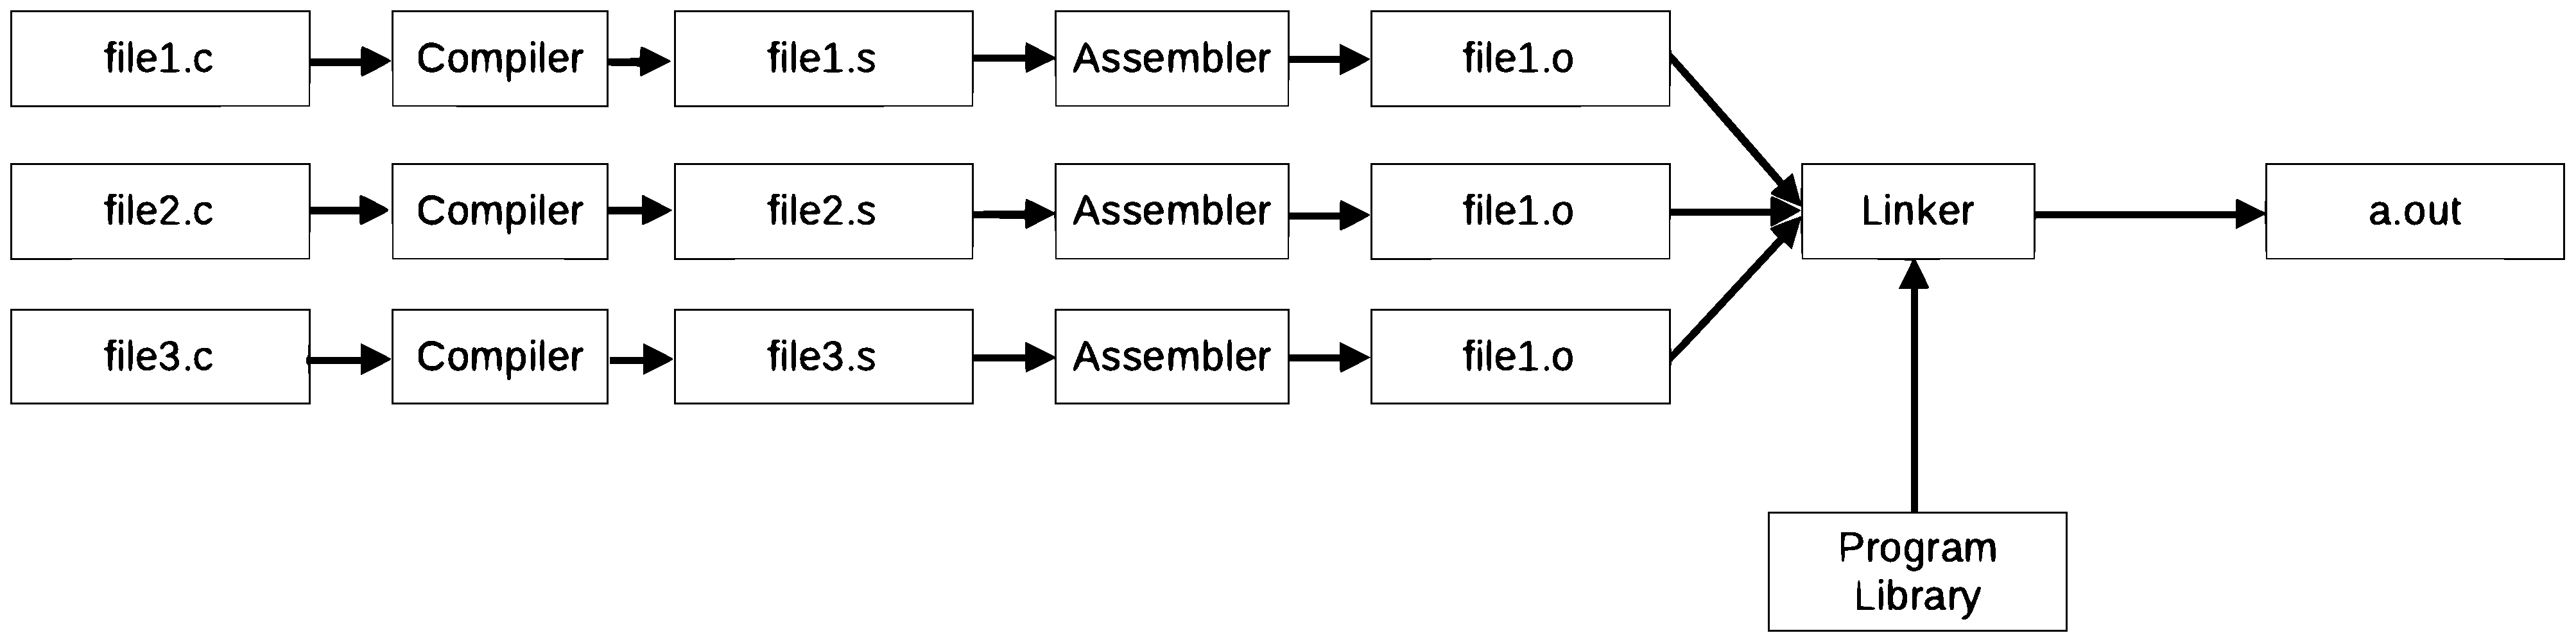
\includegraphics[scale=0.22]{figures/steps-of-compilation.eps}
\caption{Steps involved in building a C program having multiple source files}
\label{fig:stepcompile}
\end{figure}

\subsection{Operating Systems}
\subsubsection{What is an Operating System?}
Generally a computer is running multiple tasks at a time. This increases the complexity of building binaries of each individual program and running them. The complexity of running multiple tasks at the same time can be understood by two examples.\\
\textbf{Example 1:} Take the case of a student taking a numerical methods exam. Generally, questions in numerical methods require us to perform certain operations repeatedly till the answer starts converging satisfactorily. The student will be required to perform such computations many times. He must make sure that his scratch-pad is neat so that the results of different iterations and questions do not get mixed up. He must also make sure that the scratch-pad is utilized efficiently, lest he will run out of space to perform more computations.\\
\textbf{Example 2:} A librarian is tasked with managing a library. This task is composed of several tasks, for example, issuing a book as per member's demand, making sure that all books are in their specific section, etc. These tasks require that the librarian create and maintain a record of every member and every piece of literature which is present in the library.\\
In each of these examples, a single human computer was given several tasks to perform which can be performed only if every individual task is dealt with without affecting other tasks. In a computer, we run multiple tasks/programs at the same time. An editor allows us to edit source files, a shell allows us to run the compiler and a linker, a document viewer allows us to read manuals, and so on. It has to be made sure that no two programs interfere with each other. As programs often acts on files, a \textit{filesystem} also needs to be in place to make sure that the files are operated on correctly. The program tasked with managing the resources of the computer and providing an environment in which programs can run is the \textit{operating system} \cite{tannenbaum2003operating}.\\
Without an operating system, all sorts of chaos can happen. A program can start interpreting the code section of another as data, and overwrite it completely. Two or more programs accessing the printer without any prioritization and buffering will result in parts of text outputted by each program getting printed. Thus, an operating system can be thought of as the crucial software responsible for maintaining order and preventing possible chaos.

\subsubsection{System and Application Software}
Certain application-independent programs like shell, editor, compilers, windowing system, etc. are shipped along with the operating system. These are called \textit{system software}. Software like web browser, games, word processors, etc. are called \textit{application software}. System software provides the environment in which application software can run. Continuing with the analogies provided in the previous two examples, if the student is to be considered as an operating system which is managing everything, then the sheet of paper and the pen he uses are the system software. The equations he scrolls are the application software. He could have scrolled them out on the furniture, or on the walls, but he uses the tools he is provided with to get the job done. Similarly, if the librarian is an operating system, then the chairs and lights in the library are analogous to system software. Members can be made to sit on the floor and read; they are simply using the tools they are provided. Clearly, while one can choose between the shell, compiler, or the window manager they wish to use, the user is not free to write their own scheduler \citep{tannenbaum2003operating}. \autoref{fig:compsyslayout} shows the arrangement of hardware and software in a typical computer.
\begin{figure}[h]
\centering
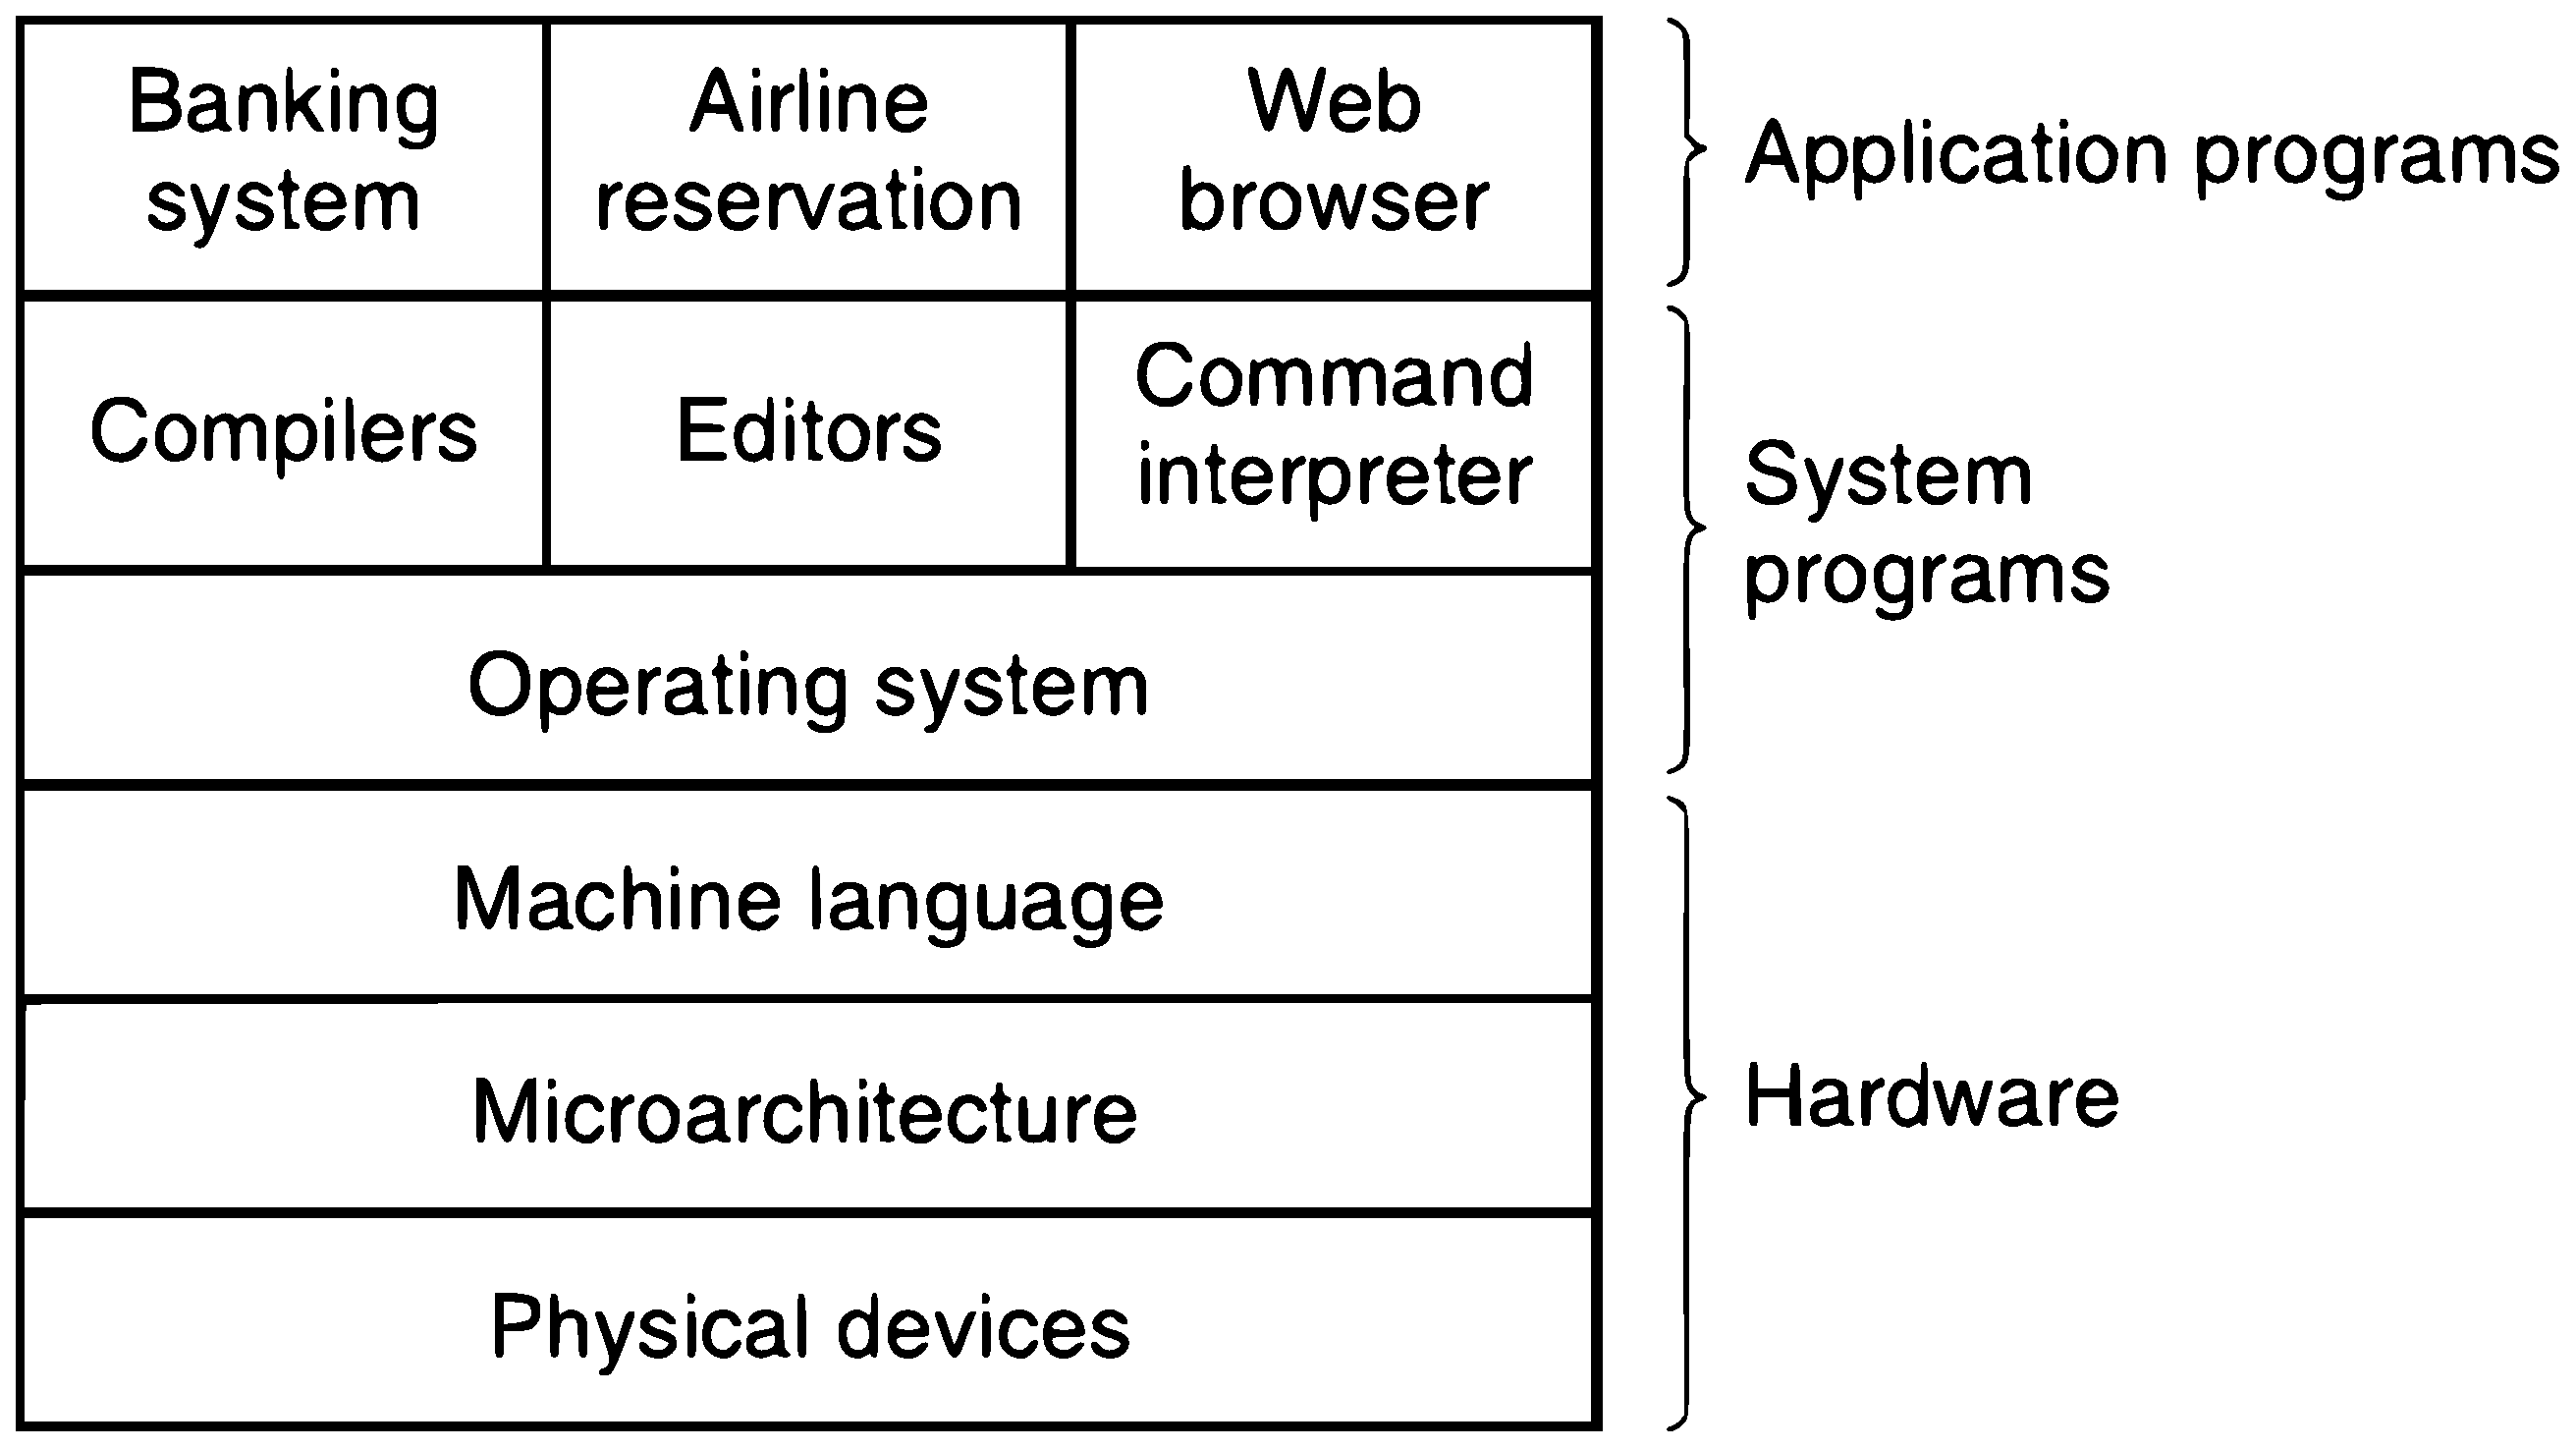
\includegraphics[scale=0.22]{figures/comp_sys_layout.eps}
\caption{Layout of a typical computer system \cite{tannenbaum2003operating}}
\label{fig:compsyslayout}
\end{figure}

\subsubsection{Functions of an Operating System}
We have described what an operating system is with the help of analogies. These analogies showed us that in operating system is the software which is responsible for managing the resources of the system. As a resource manager, the operating system has to make sure that programs do not interfere with each other. As most of the operating system today support multiple users, it becomes important that the resources allocated to each user are managed carefully. This becomes important in large organizations like universities and industries, where multiple computers are connected to a single server. This type of resource management involves sharing of resources or \textit{multiplexing}. There are two types of multiplexing: time multiplexing and space multiplexing. Time multiplexing involves allocating a specific a unit of time for each program to use the CPU. It also involves accessing I/O devices based on priority by various programs.  Space multiplexing involves giving each user (or a program) a part of the resource. An example would be the storing of all programs in main memory. This way, they can easily be time multiplexed to use the CPU and memory is not entirely given to one program only. Secondary memory like hard disks are also space multiplexed by giving each user some disk space in which they can store and organize their files.\\
Operating systems also perform the function of extending the capabilities of the machine so as to make it pleasant to deal with. When a programmer, or an ordinary user use a computer, they should be only considered with getting their job done. They should not have worry implementing a driver for hard disk, monitor, and other peripherals. Operating systems extend the instruction set of the machine by providing utility functions which allow a programmer to easily use the resources of the computer. The most fundamental utility functions are called \textit{system calls}. Examples would be \verb|read| and \verb|write| system calls in UNIX-like operating systems. These system calls are used by programs to access and operate on various files and peripherals like the screen. By providing the programmer with system calls and by setting up an environment in which work can easily be done, operating system extend the capabilities of the machine. One can say that operating systems provide the user with a virtual machines which is easier to deal with \cite{tannenbaum2003operating}.  

\subsection{A Brief History of Computers, Programming Languages, and Operating Systems}
Knowing about the history of computers is important for several reasons. Tannenbaum \cite{tannenbaum2003operating} explained the importance of learning about old systems with the example of contiguous memory allocation:
\begin{quotation}
\textit{...history may repeat itself in computer science as new generations of technology occur. Contiguous allocation was actually used on magnetic disk file systems years ago due to its simplicity and high performance (user friendliness did not count for much then). Then the idea was dropped due to the nuisance of having to specify final file size at file creation time. But with the advent of CD-ROMs, DVDs, and other write-once optical media, suddenly contiguous files are a good idea again. For such media, contiguous allocation is feasible and, in fact, widely used. Here all the file sizes are known in advance and will never change during subsequent use of the CD-ROM file system. It is thus important to study old systems and ideas that were conceptually clean and simple because they may be applicable to future systems in surprising ways.}
\end{quotation}
A lesson in the history also allows a person to understand the reason behind the design of present computers. For example, after reading the design of DEC's PDP-11, it can be seen how it influenced the design of x86 family of processors \cite{supnik2004simulators}.\\
History of computers involve studying their evolution. Just like a study of human history consists of the study of various civilizations and generations,  a study of computer history involves the study of various generations of computers. Beginning of a new generation are marked with the usage of newer, better, and reliable technology in comparison to the previous generation. The technology most  used for this classification is the hardware. By using hardware as the basis for classification, most authors divide computer history into five generations, starting in 1951 with the launch of UNIVAC I \citep{ionescu2015categories}. The \autoref{table:compgen1} is an excerpt from one such detailed table giving the history of computers \cite{friedman1992babbage}. 
\begin{table}[H]
\caption{Generations of Computers on the Basis of their Hardware}\label{table:compgen1}
\begin{center}
\begin{adjustbox}{width=1.0\textwidth,center=\textwidth}
\begin{tabular}{|c|c|c|c|}
\hline
\textbf{Generation} & \textbf{Year} & \textbf{Technological Features} & \textbf{Examples}\\
\hline
1st Generation & 1951-1960 & Vacuum tubes & UNIVAC I, IBM 650\\
\hline
2nd Generation & 1959-1965 & Transistors & IBM 1401, IBM 7094\\
\hline
3rd Generation & 1964-present & Integrated circuits & IBM 360, PDP-11 (16-bit minicomputer)\\
\hline
4th Generation & 1971-present & VLSI, Microprocessors & Altair 8800, Commodore VIC-20\\
\hline
5th Generation & Present-future & Parallel processing architecture & Computers using Pentium or higher\\
\hline
\end{tabular}
\end{adjustbox}
\end{center}
\end{table}
By using programming languages and operating systems as the basis for classification, we arrive at similar results \cite{tannenbaum2003operating}. This type of classification is more useful in context of the present report and, therefore, it will be discussed from here on.

\subsubsection{The Zero Generation Computers (1645--1945)}
This generation of computers came before the invention of digital computers. In reality, if one takes into consideration human computers and mechanical calculators, then computers have been around since eternity. The oldest known mechanical computer would be the Antikythera mechanism from 87 BC which was supposedly used to predict astronomical positions and eclipses \cite{ionescu2015categories}\cite{10.1115/1.2018-SEP1}. More examples of early calculators would be abacuses and slide rules, the latter being used well into the 1970's and is credited for putting the man on the Moon \cite{stoll2006slide}. \\
The first mechanical calculator would be Pascal's calculator (or Pascaline). It was capable of addition and subtraction, and multiplication and division using repeated addition and subtraction, respectively \cite{chapman1942pascal}.\\ 
The most significant mechanical computers were Charles Babbage's difference engine and analytical engine. Construction of the difference engine began in 1819 and a small portion of it was completed and demonstrated in 1822. The difference engine used the method of finite differences to interpolate functions \cite{dasgupta2014began}. The analytical engine was a more complex machine which introduced several new concepts like program and memory. Although not completed during Babbage's lifetime, the analytical engine was shown to be programmable by Ada Lovelace \cite{tannenbaum2003operating}.\\
Mechanical differential analyzer's and their analog counterparts used during the two world wars were also programmable. The integrators and differentiators they were made up of were linked together to model systems through their differential equations. The output was a plot of the system's output with respect to input. As signals out of blocks were feeble, they were passed through an amplifier before being passed to the next block. Each of these amplifications were to be taken into account when interpreting the output \cite{robinson_t_2005_918318}.\\
For each of these mechanical computers, the concept of a program was plugboard wiring or positions of mechanical linkages. The concept of an operating system, or even programming languages, didn't exist yet.

\subsubsection{The First Generation Computers (1945--1955)}
Work on developing mechanical digital computers continued until 1945. These early calculating engines were made up of relays, which were later replaced by much faster vacuum tubes. One of the most remarkable person involved with the first generation computers was Konrad Zuse. In 1936, he completed a relay based mechanical computer named \textit{Z1} in his parent's basement. It was a floating point mechanical calculator which could be programmed using perforated 35 mm films. Later, he designed Z2 and Z3, the latter having 2600 relays, 22-bit word length and operated at frequency of 5-10 Hz \cite{morelli2001dalle}. While working on Z4, he found that programming on machine code was hard. He then designed the world's first high-level language named \textit{Plankalkül} \cite{hellige2013geschichten}.\\
Meanwhile in United States, J. Presper Eckert and John Mauchly invented the ENIAC (Electronic Numerical Integrator and Comparator) at the University of Pennsylvania in 1945. It was the first general-purpose programmable digital computer. Both the hardware and software of the ENIAC was different from modern computers. It was made up different machines each capable of performing a specific arithmetic operation. It was programmed by wiring a plugboard and three portable function tables. Each function table had 1200 ten-way switches which were used to enter a table of numbers. Programming was done only by the members of the ENIAC team after the program has been thoroughly tested \cite{cruz2013eniac}. In 1996, on the 50th anniversary of the ENIAC, using CMOS technology, a 7.4 mm x 5.3 mm chip with the same functionality as the ENIAC was successfully built \cite{6302808}.\\
EDVAC (Electronic Discrete Variable Automatic Computer), ENIAC's successor, was also designed by Eckert and Mauchly before ENIAC got completed. It was put into operation in 1951. Eckert and Mauchly, and the design team of the EDVAC were joined by the famous mathematician John von Neumann who acted as a consultant. Neumann later wrote a 101 page incomplete monograph titled \textit{The First Draft of a Report on the EDVAC} \cite{von1993first}. In it he described a computer architecture in which program and data are stored in the same memory space. This architecture is called the \textit{von Neumann architecture}. A machine using this architecture is called a \textit{stored program} machine. The first computer to implement von Neumann architecture was the EDSAC at Cambridge. A computer architecture having program and memory in different memory spaces is called the \textit{Harvard architecture}.\\ 
It was soon realized that programming computers in machine code by interlinking various arithmetic and logic blocks using a plugboard/control panel was inefficient. Computers produced near the end of this generation had, besides a plugboard, a punch card input-output unit. User, using a modified typewriter, punched holes into cards. These cards were fed into a card reader. The card reader read the cards using optical sensors: light shown on the cards passed through the punches and activated the optical sensor below them. This was interpreted as the binary '1'. The rest of the optical sensors registered a binary '0'. The resulting binary was fed into the main memory of the computer, usually a magnetic drum. Results were punched out on the cards using an opposite mechanism.\\
An example of a machine which was operated this way was the IBM 650. The IBM 650 was a stored program machine. It had console from which the machine could be programmed in machine code using octal switches and its state during program execution could be seen. Data was written and read from its magnetic drum memory by the IBM 533 input-output unit using punched cards \cite{andree1958programming}. Donald Knuth dedicated his magnus opus \textit{The Art of Computer Programming} to an IBM 650 which he used to learn programming while an undergraduate at the Case Institute of Technology \cite{knuth1997art}.
It should be noted that besides the complexity of programming these early computers, the task of debugging a program and fixing the machine was also hard. Considerable time was lost in finding the vacuum tube which has burned out.

\subsubsection{The Second Generation Computers (1955--1965)}
Invention of the transistor in 1947 ushered a new era in the field of electronics and computer science. Vacuum tubes were replaced by transistors to build amplifiers and digital logic circuits. The small size and high power efficiency of transistors meant that computers, instead of requiring a hall to be fit into, could now be fit into a room. As the reliability of transistors was high in comparison to vacuum tubes, it meant that computers made using them could easily be mass produced and sold without the customers worrying about repairs for a long time. Computers of this generation were called \textit{mainframes} \cite{tannenbaum2003operating}. Two important examples of mainframes from this generation would be the IBM 1401 and 7094 computers.\\
Around this same time, assembly language gained prominence and high-level languages like COBOL and FORTRAN were introduced. Assembly language is still used today to develop firmware (BIOS, embedded system software). Time critical parts of software used in aeroplanes, fighter-jets, rockets, etc. are still written in assembly language. Inline assembly code can be found in the source code of the Linux kernel. FORTRAN is also still used  for scientific calculations in experimental physics and other applied technical domains. It has been called the "mother tongue of scientific computing" \cite{halpern1993large}. COBOL, on the other hand, is a nearly obsolete language: these days COBOL programs can only be found in mainframes in various business firms. They haven't been replaced by programs written in other languages because the cost of replacing a known technology which has been working reliably for the past five decades is very risky \cite{mitchell2006cobol}.\\ 
To program these computers, a programmer would first write the program on paper in either assembly language or FORTRAN. Then, he would type it out on a machine like the IBM 029, which would encode each keystroke on the typewriter by punching the cards. In the end, the programmer would be having a deck of cards having his program. This deck was fed into a card reader connected to the computer. Here, the deck was read and the program was stored in the main memory of the computer. The computer then executed the program and the results were stored in its main memory. To print out the results, a printer would read the memory and print the output on a roll of paper. The next deck of cards containing another program/job was then loaded and executed by the computer.\\
It should be noted that while the cards were being read and the results were being printed, the computer was sitting idle. That is, it was doing no data processing during the time it was reading decks, copying them to memory, or printing data from memory. To reduce this waste of time, \textit{batch system} was invented. In it, an expensive computer like the 7094 which was good at numerical calculations was were used solely for executing programs. The task of card reading and writing was relegated to computers like the 1401 which were good at reading cards to tape, copying data and reading tape. A collection of decks, each containing different jobs/programs, was called a batch. It was fed into a 1401 which copied the programs in the batch to a magnetic tape. An operator would then take this tape and connect it to the tape drive of the 7094. The 7094 then ran a special program which would read each program on the first tape one-by-one and write their output to a second tape instead of printing them out. This program was a precursor to modern operating systems. When a batch of job had been executed, the second tape was taken by an operator who would connect it to the tape drive of the 1401. Its contents were read and printed on a roll of paper. Meanwhile, another operator would connect a tape containing another batch of job to the tape drive of the 7094 \cite{tannenbaum2003operating}.

\subsubsection{The Third Generation Computers (1965--1980)}
Miniaturization of computers continued with the introduction of integrated circuits (ICs). The first monolithic IC was invented by Robert Noyce in 1959. The first prominent use of integrated circuits was made in the construction of the Apollo Guidance Computer (AGC). Consultants hired by NASA mathematically proved that a computer made using ICs, transistors, and diodes would have a very high probability of failure. Their calculations used the assumed failure rate of these components. Eventually, Eldon C. Hall, leader of the hardware designing team for the AGC at MIT and an advocate for the use of integrated circuits, convinced NASA that such mathematical calculations were bogus as they were not using the actual failure rate of the aforementioned components. Also, measuring the actual failure rate of the components would take years which would put them a step back in the space race. He eventually prevailed and the AGC was built using the latest semiconductor technology. The computer's main memory was made out of core rope. On it was stored the operating system which controlled various systems of the command and lunar module. It had a scheduler which executed various programs based on their priorities and in case of a failure, it saved the state of the machine, and restarted it. Both the hardware and the software of the computer proved to be highly reliable and had a 100\% success rate \cite{hall1996journey}.\\
Meanwhile, IBM was dealing with the complexity of producing, marketing and supporting two completely different lines of computers: commercial computers, like the 1401, and scientific computers, like the 7094. Both lines had different architecture and instruction set. Customers who wanted to shift from lower end to higher end computers found it challenging to port their entire code base to a newer machine. IBM attempted to reduce this complexity by releasing a single line of computers, the System/360. The machine could be used for both commercial and scientific computing. It was all a matter of the configuration the user wanted. As the architecture and the instruction set of the machine was same for all the lines, users no longer had to worry about porting their code base from one line to another \citep{tannenbaum2003operating}.\\
IBM introduced a new operating system, OS/360, for its System/360 line. It was able to keep the CPU busy 100 percent of the time by assigning it jobs to do while the job it was currently on was waiting for I/O to complete. Each job was stored in its own memory partition and special hardware was used to prevent one job from altering the contents of others. This was called multiprogramming \cite{tannenbaum2003operating}.\\
Though OS/360 introduced several new concepts, it was still fundamentally a batch system. To reduce the time for which programmers had to wait to get their job done, the concept of timesharing was introduced. The most popular timesharing operating system was the Compatible Time Sharing System (CTSS). It was developed at the MIT Computation Center and used a modified IBM 7090 mainframe. It had a kernel, which was the program responsible for scheduling between different users, had system calls which could be called by software interrupts, and implemented memory protection schemes. The scheduler had a quantum time unit of 200 ms, and was responsible for deciding the user who was to be allotted computer time, the amount of time to be allocated, keeping track of activities of all users, and the net charges for the user. The filesystem of CTSS gave each user their own directory. Users would issue commands using a teletype-writer (also called a terminal) like the ASR 33. When the scheduler executed a user's command, the output was displayed on the paper in the typewriter \cite{peterson1985operating}\cite{tannenbaum2003operating}.\\  
Success of the CTSS made MIT, Bells Labs, and General Electric join hands to develop a \textit{computer utility}. The idea was that just electricity and water are utilities which people access by tapping into some main channel, similarly computers should be a utility. The designers imagined a single powerful computer providing computing power to users in a large area. The computer of choice was a GE-645 mainframe and the operating system designed was called MULTICS (MULTiplexed Information and Computing Service). MULTICS introduced several novel ideas at that time but overall it was a disaster. The enormous size and complexity of the system which was mostly written in PL/I language, compiler for which barely worked, made MULTICS unusable. Ken Thomson referred to MULTICS as "\textit{overdesigned and overbuilt and over everything. It was close to unusable. They [Massachusetts Institute of Technology] still claim it's a monstrous success, but it just clearly wasn't}" \cite{seibel2009coders}. General Electric quitted the computer business and Bell Labs withdrew its efforts into developing it. MIT persisted and developed a functional version of MULTICS by mid 1970's which was installed in over 80 institutions around the world \cite{tannenbaum2003operating}.\\
Around this time, minicomputers were rising in popularity. These computers were smaller and cheaper than a mainframe. Digital Equipment Company (DEC) Programmed Data Processor (PDP) line of minicomputers was extremely popular. Ken Thompson, who had earlier worked on the MULTICS project, started developing an operating system for a PDP-7 so that he could play \textit{Space Wars} on it \cite{torvalds2001just}. He was soon joined by Dennis Ritchie. Their goal was to design an operating system for a single user which had all the good parts of MULTICS and none of its bad parts. The resulting operating system was called UNIX which was a pun on the name MULTICS. On the influence of MULTICS on UNIX, Thompson had the following to say: "\textit{the things that I liked enough (about Multics) to actually take were the hierarchical file system and the shell — a separate process that you can replace with some other process}" \cite{seibel2009coders}.\\
UNIX quickly became popular. It was soon decided that UNIX should be ported to a newer and more powerful PDP-11. However, as most of it was written in assembly language which was tied to the architecture of PDP-7, a need for developing a new systems programming language was felt. This prompted Dennis Ritchie to write a new programming language, C, which was specifically designed to be small, portable, and powerful. Ritchie, along with Brian Kernighan, wrote \textit{The C Programming Language}, 2nd (and last) edition of which is still considered as the \textit{de facto} standard for ANSI C and for writing technical books \cite{ritchie1988c}.

\subsubsection{The Fourth Generation Computers (1980 - Present)}
Development of a complete processor on a square centimetre of silicon was made possible with large scale integration (LSI) technology. These processors on a single integrated circuit were called microprocessors, and the computers using them were called microcomputers. Architecturally, both minicomputers and microcomputers were the same. However, when it came to price, microcomputers were significantly cheaper. Further improvements in miniaturization of technology allowed computer manufacturers to get rid of mechanical components and replace them with electronic ones. An example would be the replacement of a teletype-writer with a keyboard and a monitor. A software called a terminal emulator is used to implement an environment in which commands and their outputs are visible on the screen.\\
Computers like the Commodore VIC-20 and Apple II started the microcomputer revolution. The competition between different companies meant that affordable computers were available to the home user. As these computers were intended for use by a single user, they were often called personal computers, a term which still persists till this day.\\
The 8086 microprocessor was released in 1978 and its cheaper version, the 8088, was released in 1979. IBM decided to enter the personal computer market by building a microcomputer around the cheaper 8088. The result was the IBM PC, which debuted on August 12, 1981 \cite{ibmarchpc} and was cloned by competing manufacturers in the following year. The IBM PC soon became the \textit{de facto} standard for PC, a fact which is true for modern PCs as well.\\
The original IBM PC (the one using 8088 microprocessor) came with two floppy disk drives, a port for attaching cassette tape recorder, and an optional hard disk drive. Software companies started producing disk operating systems (DOS) which came in floppy drives. User had to insert the floppy drive before turning the computer on. A few examples of DOS were CP/M-86 by Digital Research, 86-DOS by Seattle Computer Products, and MS-DOS by Microsoft. MS-DOS was created by the author of 86-DOS, Tim Patterson.\\
Up till UNIX Version 6, the source code of UNIX was widely available with AT\&T license and was frequently studied in universities. Berkley University modified their copy of source code to a great extent to make UNIX suitable for their own requirements. AT\&T (Bell Labs were a part of it) realized that UNIX can be commercialized. They issued Version 7 with a license which prohibited universities from studying its source code. These led to a legal dispute between AT\&T and Berkley University. Meanwhile, Andrew Tannenbaum wrote his own version of UNIX from scratch for use in the operating systems course he taught at Vrije Universiteit Amsterdam. He called it MINIX and it, along with his book \textit{Operating Systems: Design and Implementation} soon became popular \cite{tannenbaum2003operating}.\\ By early 1990's, IBM PCs with 80386 (or i386), which was a 32-bit processor with hardware for multitasking, were becoming popular. MINIX was originally designed for the original IBM PC, so it could not use the full potential of the newer, powerful hardware. Seeing these limitations of MINIX, Linus Torvalds, then a student at University of Helsinki, developed an operating system called Linux which was inspired from MINIX. It used MINIX's filesystem but had a monolithic architecture (as opposed to MINIX's microkernel), and was released in August of 1991. Since then, it had become the largest open source project in the world. Linux based distros are used on servers, smartphones, personal computers, etc \cite{torvalds2001just}.    

\subsection{The 8086 Microprocessor from a Programmer's Point of View}
The 8086 microprocessor was launched on June 8, 1978. It subsequently gave rise to the x86 family of processors which have been the most successful processors till date. Though the original IBM PC had an 8088 instead of an 8086, we will restrict our discussion to the PCs using 8086 as that is more relevant.

\subsubsection{Physical Specifications}
The 8086 microprocessor was available as a 40 pin DIP IC, often in ceramic casing. Its pin configuration is shown in \autoref{fig:8086pinconfig}.\\
The 8086 microprocessor can be powered using 5 volt power source. Its standard operating speed is 5 MHz, but versions with clock rate of 8 MHz and 10 MHz are available.\\ 
\begin{figure}[h]
\centering
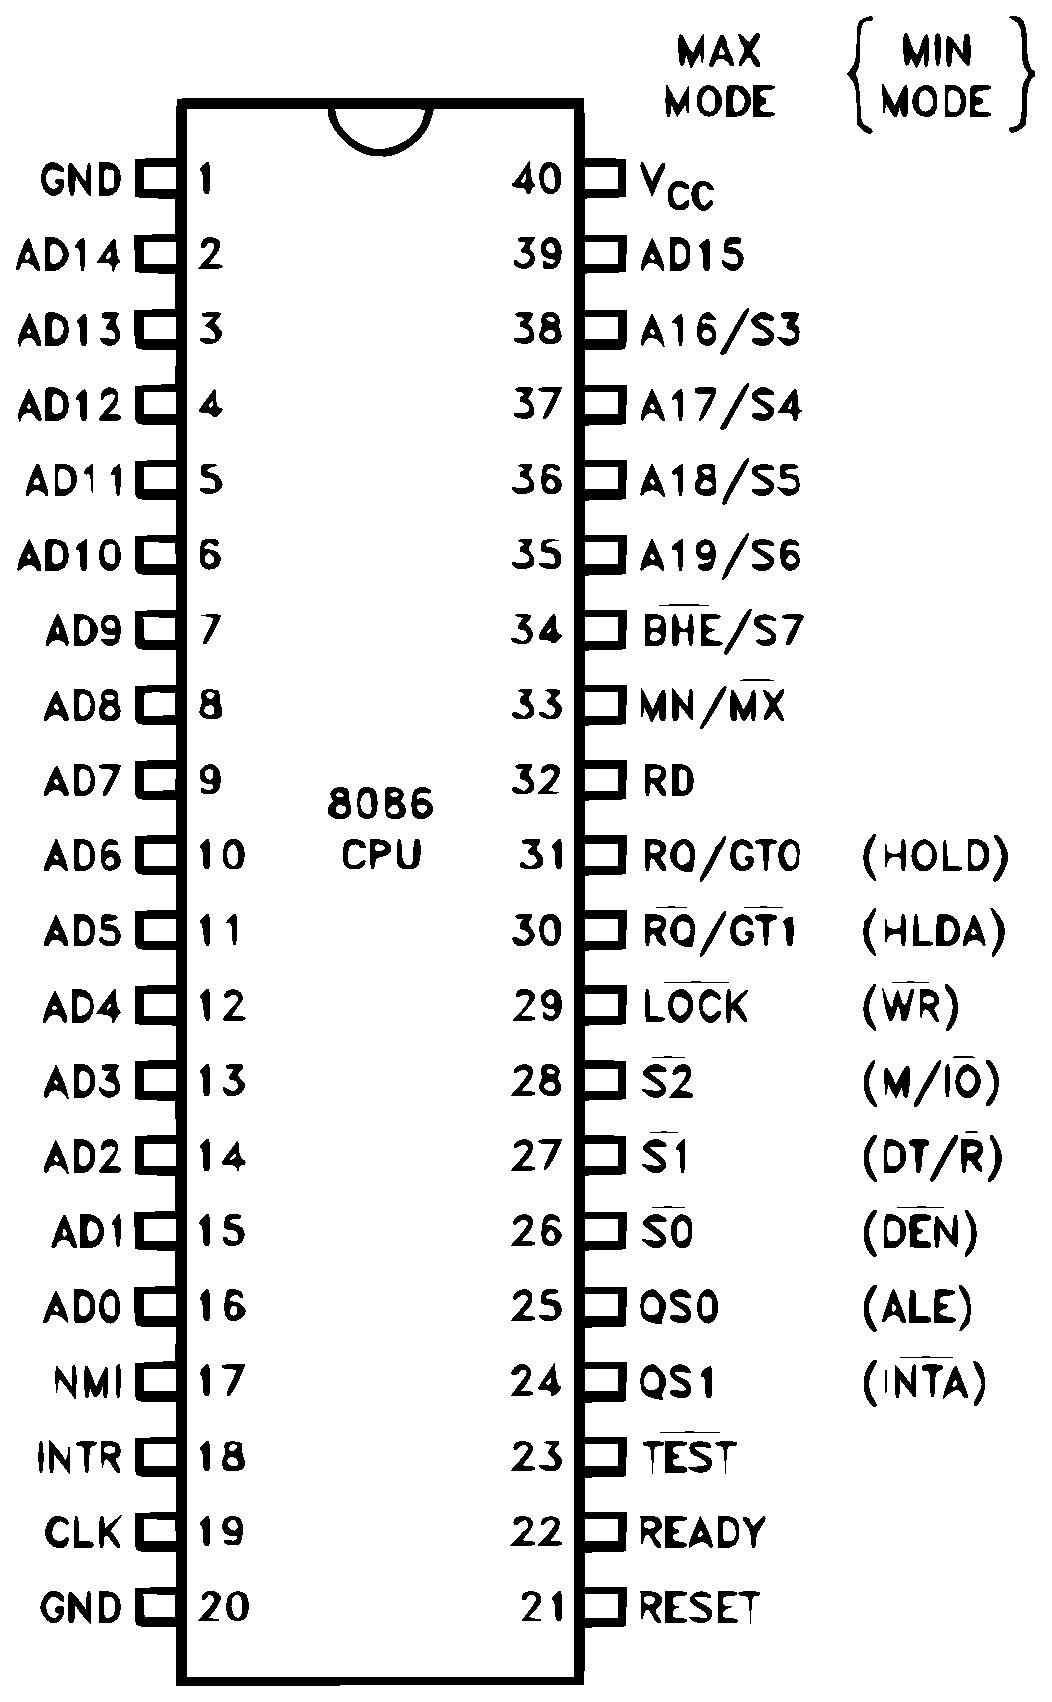
\includegraphics[scale=0.25]{figures/8086pinconfig.eps}
\caption{Pin configuration of the 8086 \cite{intel19908086}}
\label{fig:8086pinconfig}
\end{figure}
The processor has a multiplexed 20-bit address bus and 16-bit data bus: 16 pins are shared between both the address and data bus. The remaining higher order 4 bits in the address bus come from physical address calculation by the bus interface unit (BIU).\\
The processor can be operated along with other processors by putting it in maximum mode. This is done by strapping its MN/$\overline{\text{MX}}$ pin to the ground. In this mode, CPU encodes its signal, which are decoded and used by the 8288 bus controller to control the system. To put the processor in minimum mode, MN/$\overline{\text{MX}}$ pin is strapped to +5V.

\subsubsection{Execution Unit and Bus Interface Unit}
In section 2.3.3 and 2.3.4 we discussed how the efficiency of computation by mainframes was maximized by using batch system and multiprogramming. The idea was to minimize the time for which the processor was idle by giving it enough jobs/programs to keep it occupied while the I/O operations were performed by cheaper machines. The concept of batch system and multiprogramming were applied in the design of the 8086 microprocessor. Instead of having a single processing unit which was responsible for fetch and writing data and instructions and execution, the 8086 has two processing units: the execution unit (EU) and the bus interface unit (BIU). The EU is responsible for executing the instructions and the BIU is responsible for fetching instructions, reading operands, and writing data to memory or to the ports. The two processors operate independently of each other thus ensuring that the EU is in operation for most of the time. The BIU has an internal buffer in which it would prefetch and store the instructions so that the EU's time is not wasted by waiting for the next instruction. This buffer is basically a queue. The size of this queue is four bytes for the 8088 and six bytes for the 8086 \cite{intel19908086}.
\begin{figure}[h]
  \centering
  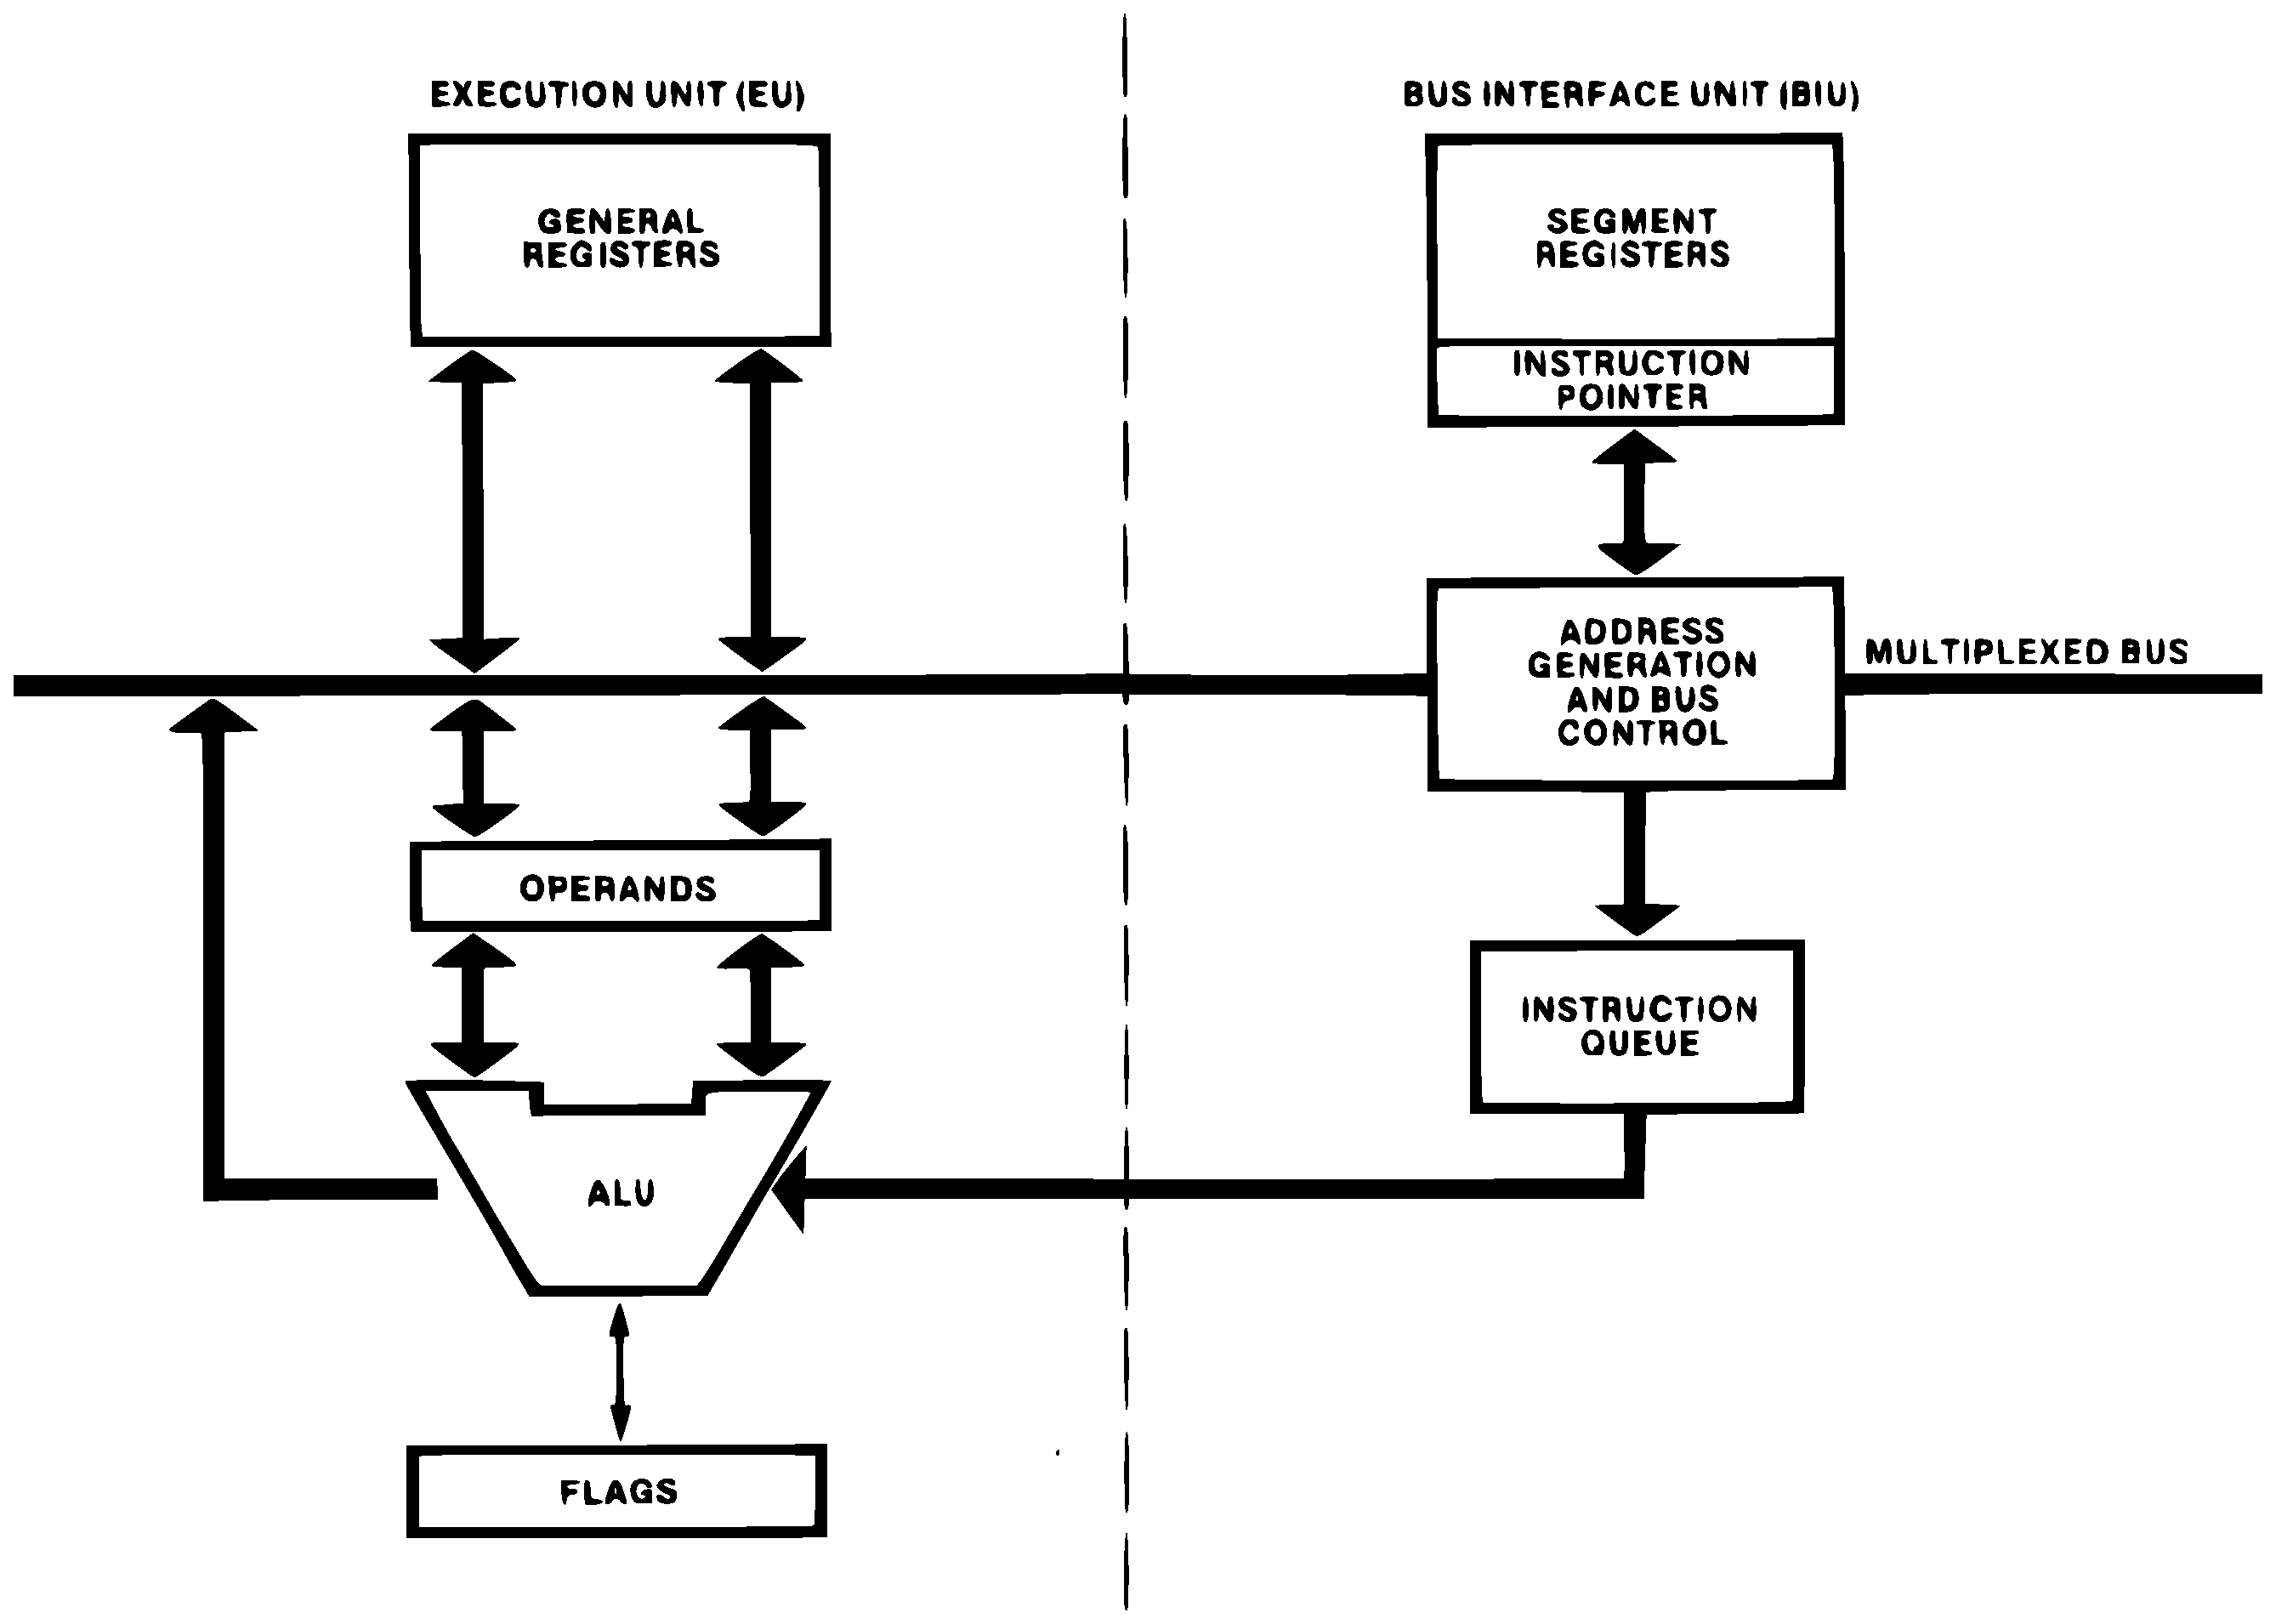
\includegraphics[scale=0.25]{figures/8086block.eps}
  \caption{Block diagram of the 8086/8088 microprocessor \cite{intel1979the}}
\label{fig:8086block}
\end{figure}

\subsubsection{Registers}
Two sets of registers are provided to both the EU and the BIU. The 16-bit registers provided to the EU are called general purpose registers. The 16-bit registers provided to the BIU are called segment registers. A 16-bit instruction pointer is also provided to the BIU.\\
General purpose registers are frequently used in arithmetic and logical calculations, and comparisons, and also for addressing data in memory. These are \verb|ax|, \verb|bx|, \verb|cx|, \verb|dx|, \verb|sp|, \verb|bp|, \verb|si|, and \verb|di|\footnote[1]{In older documents and source codes, one would find that instructions, operands, and hexadecimal numbers were exclusively written in uppercase. Nowadays, assembly source codes are written both in lowercase and uppercase literals. Due to the availability of different typesetting software, many newer documents also make use of both the cases for instructions, operands, and hexadecimal numbers. In this report and the source code for this project, instructions, register names, and hexadecimal numbers are exclusively written in lowercase. A breaks in this convention might be observed, especially at places where older documents are referenced, and in figures. In the end, the case which appears to be pleasant to the eyes and is relevant is used.}. Each of \verb|ax|, \verb|bx|, \verb|cx|, and \verb|dx| could be split into two 8-bit registers thus providing a total eight 8-bit registers. This is shown in \autoref{fig:8086gpr}. \verb|ax|, \verb|bx|, \verb|cx|, and \verb|dx| are used in computations and comparisons. One can say that there are four 16-bit accumulators in the 8086 processor. The \verb|ax| register along with \verb|dx| is used to store the results of operations. After 16-bit multiplication, the product's low word is stored in \verb|ax| and high word is stored \verb|dx|. After 16-bit division, the quotient is stored in \verb|ax| and the remainder in \verb|dx|. \verb|cx| register is used as a counter in loop operations.\\
\begin{figure}[h]
\centering
  \begin{subfigure}{.5\textwidth}
  \centering
  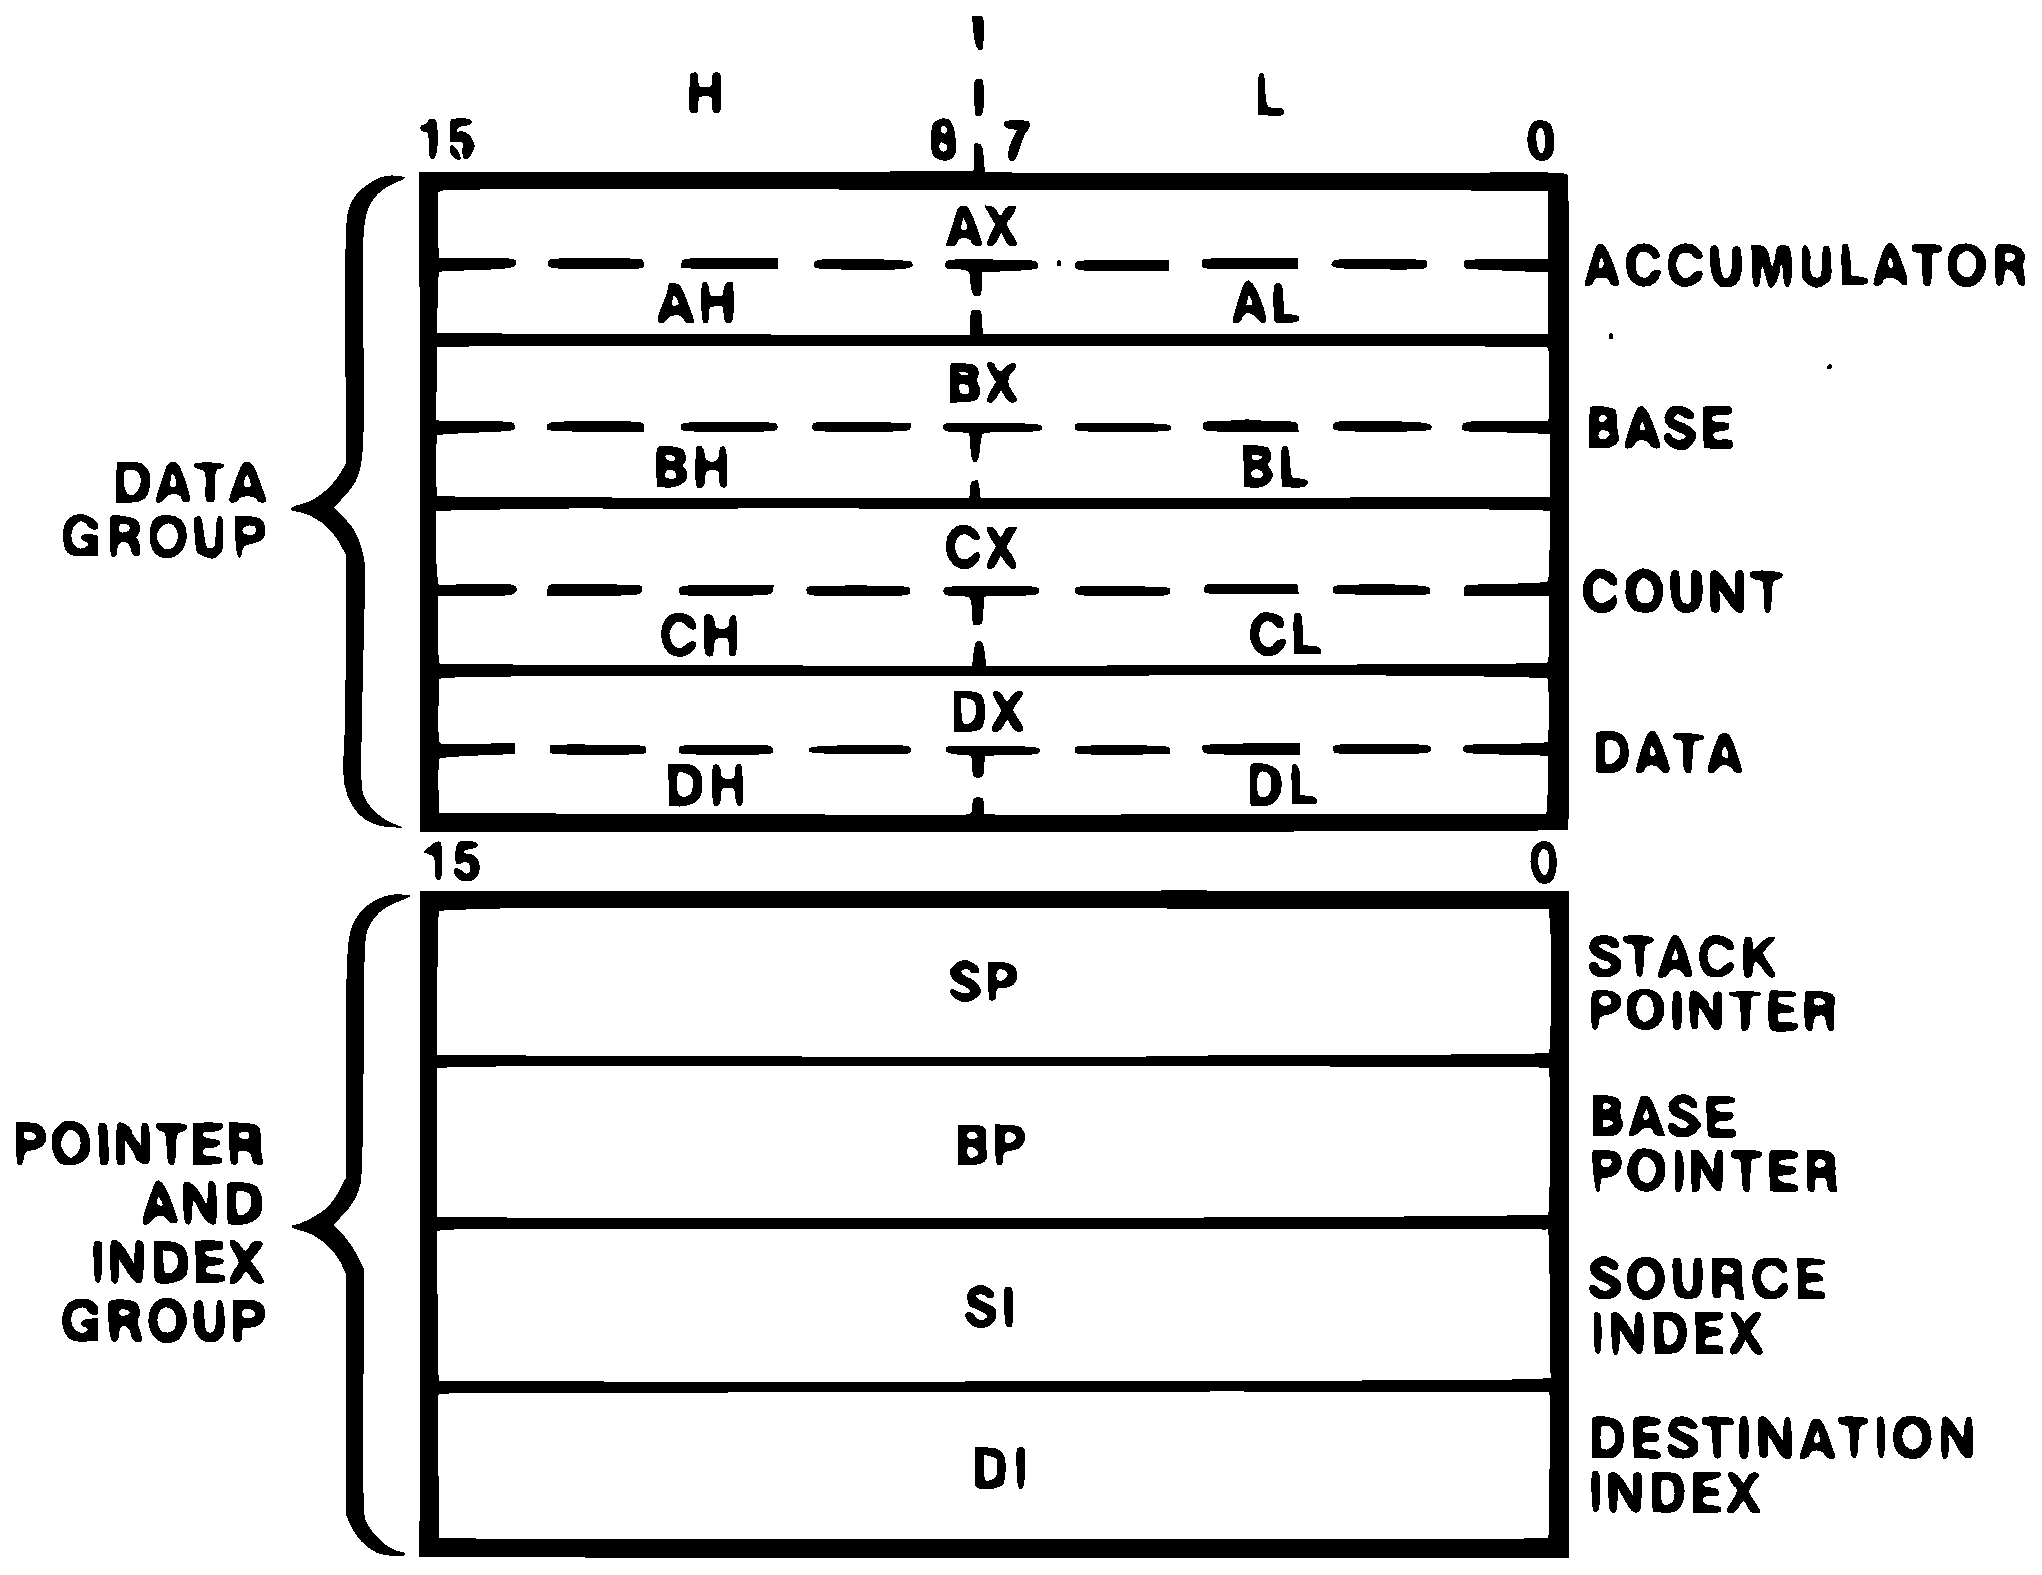
\includegraphics[scale=0.25]{figures/8086gpr.eps}
  \caption{General purpose registers}
  \label{fig:8086gpr}
  \end{subfigure}%
  \begin{subfigure}{.5\textwidth}
  \centering
  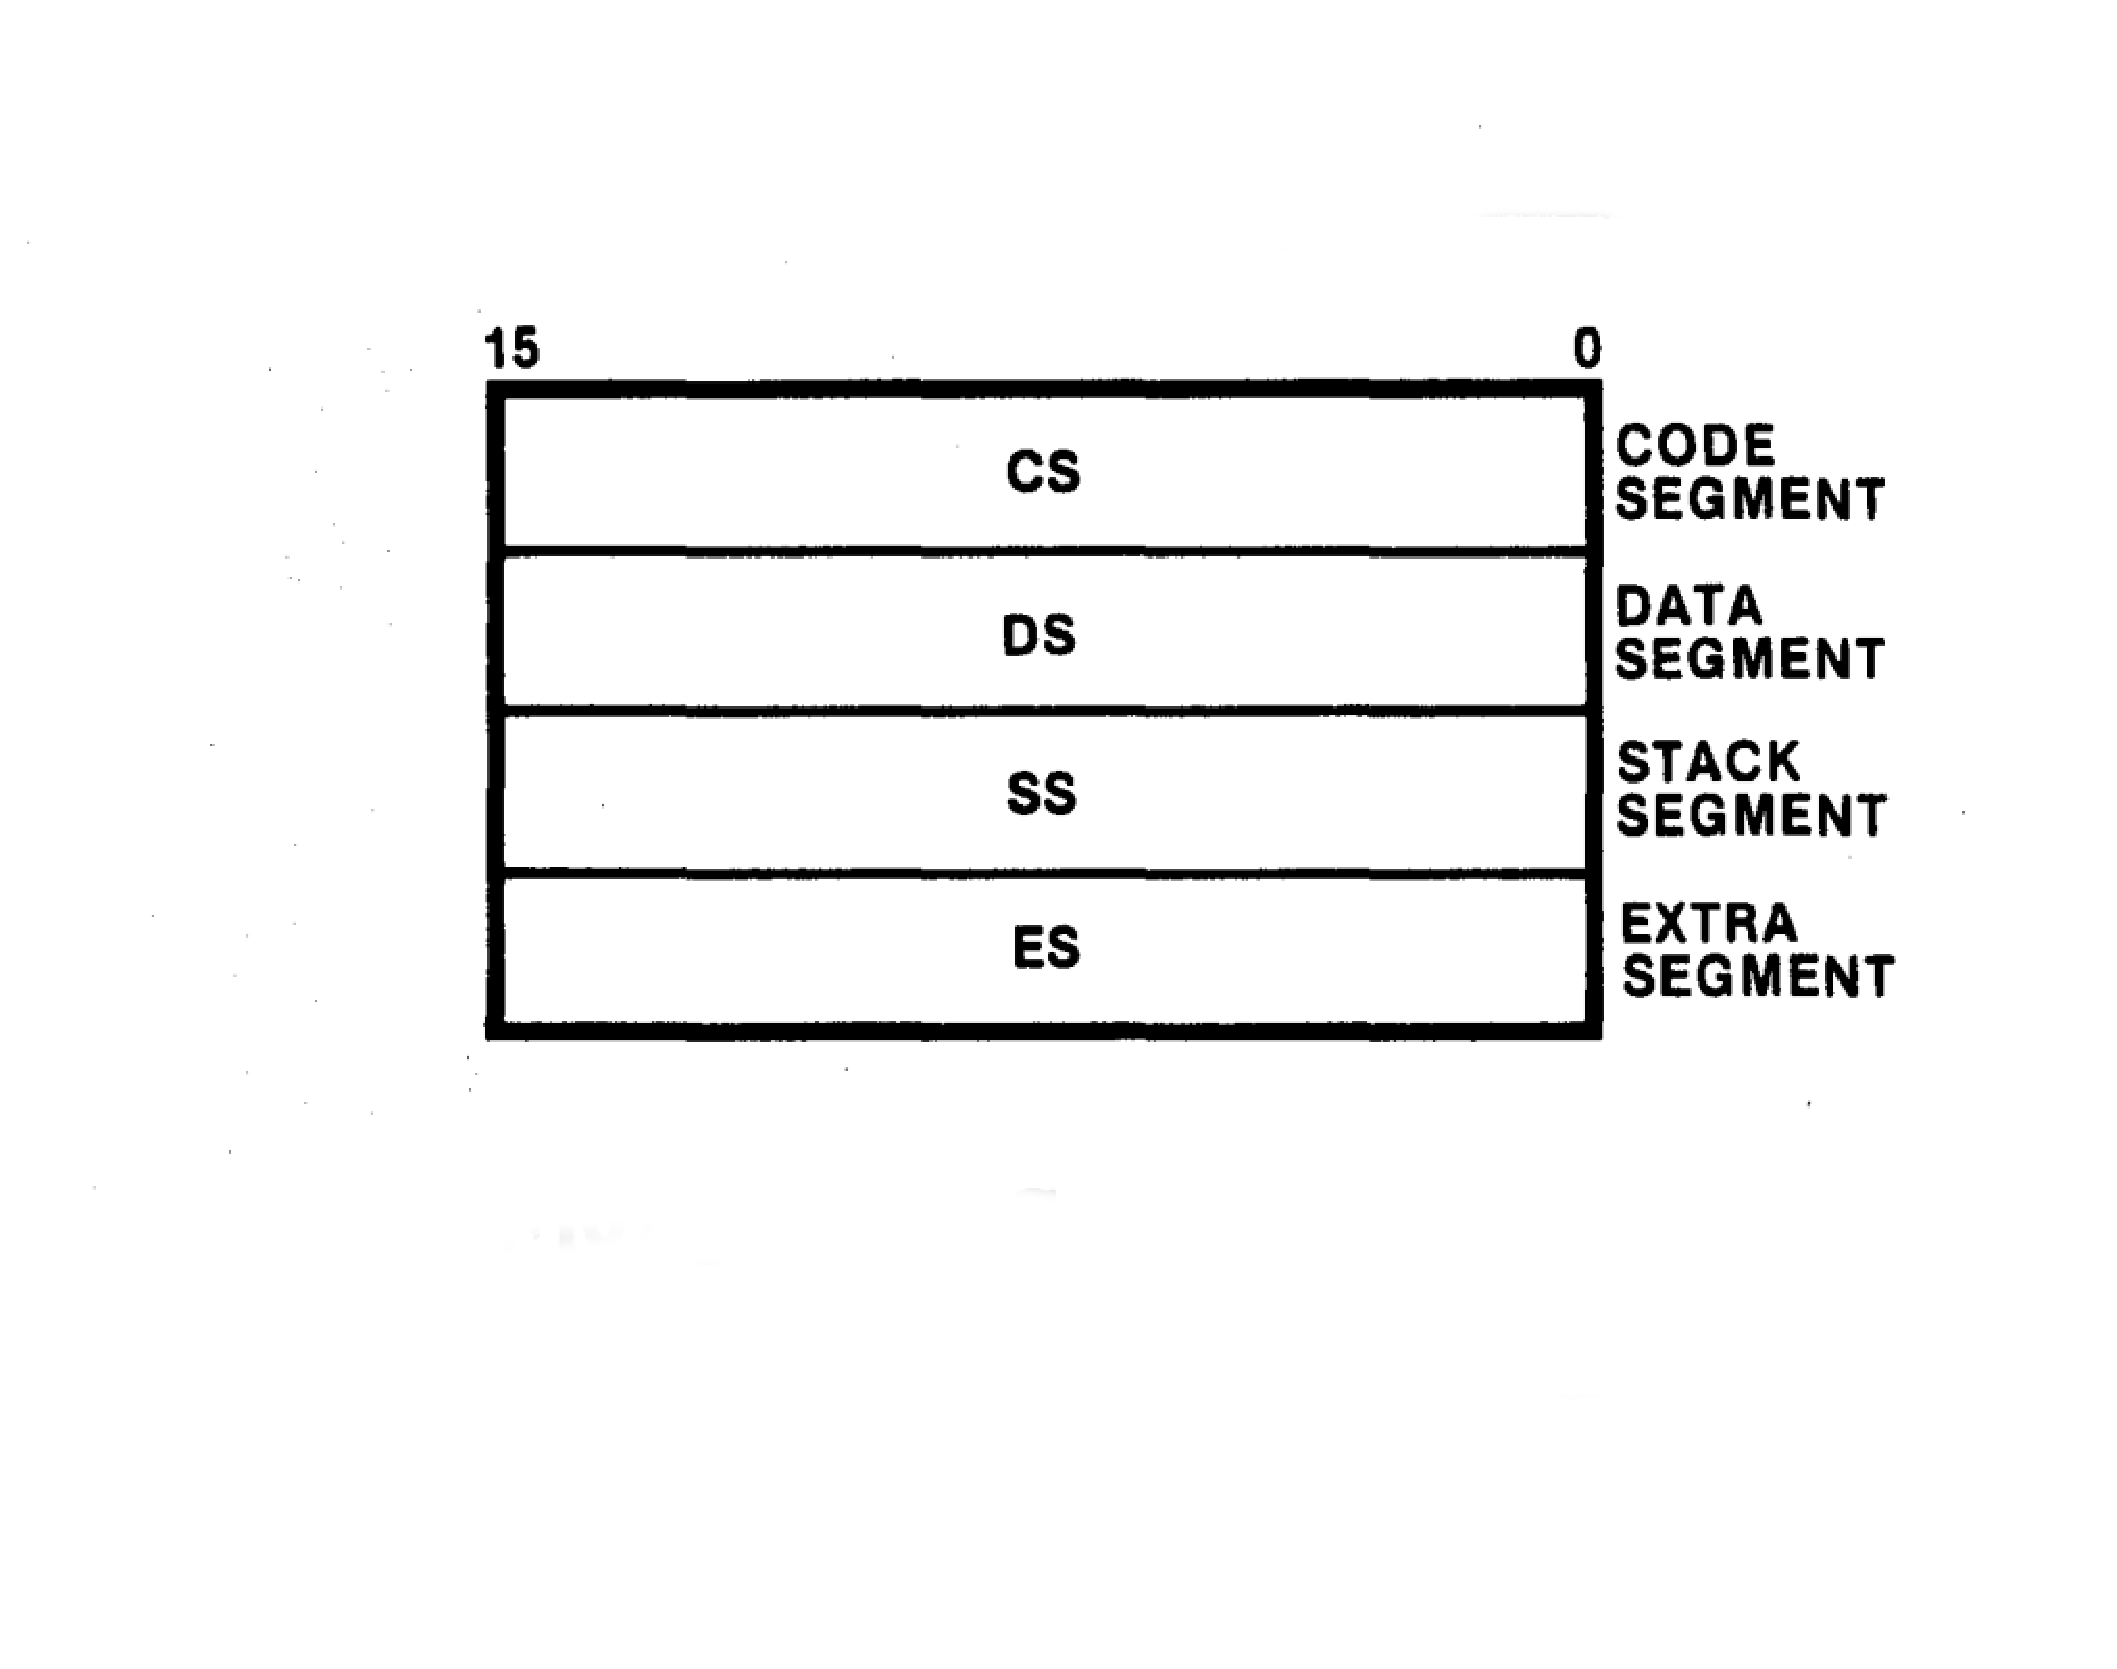
\includegraphics[scale=0.25]{figures/8086segr.eps}
  \caption{Segment registers}
  \label{fig:8086segr}
  \end{subfigure}
  \newline
  \begin{subfigure}{0.9\textwidth}
  \centering
  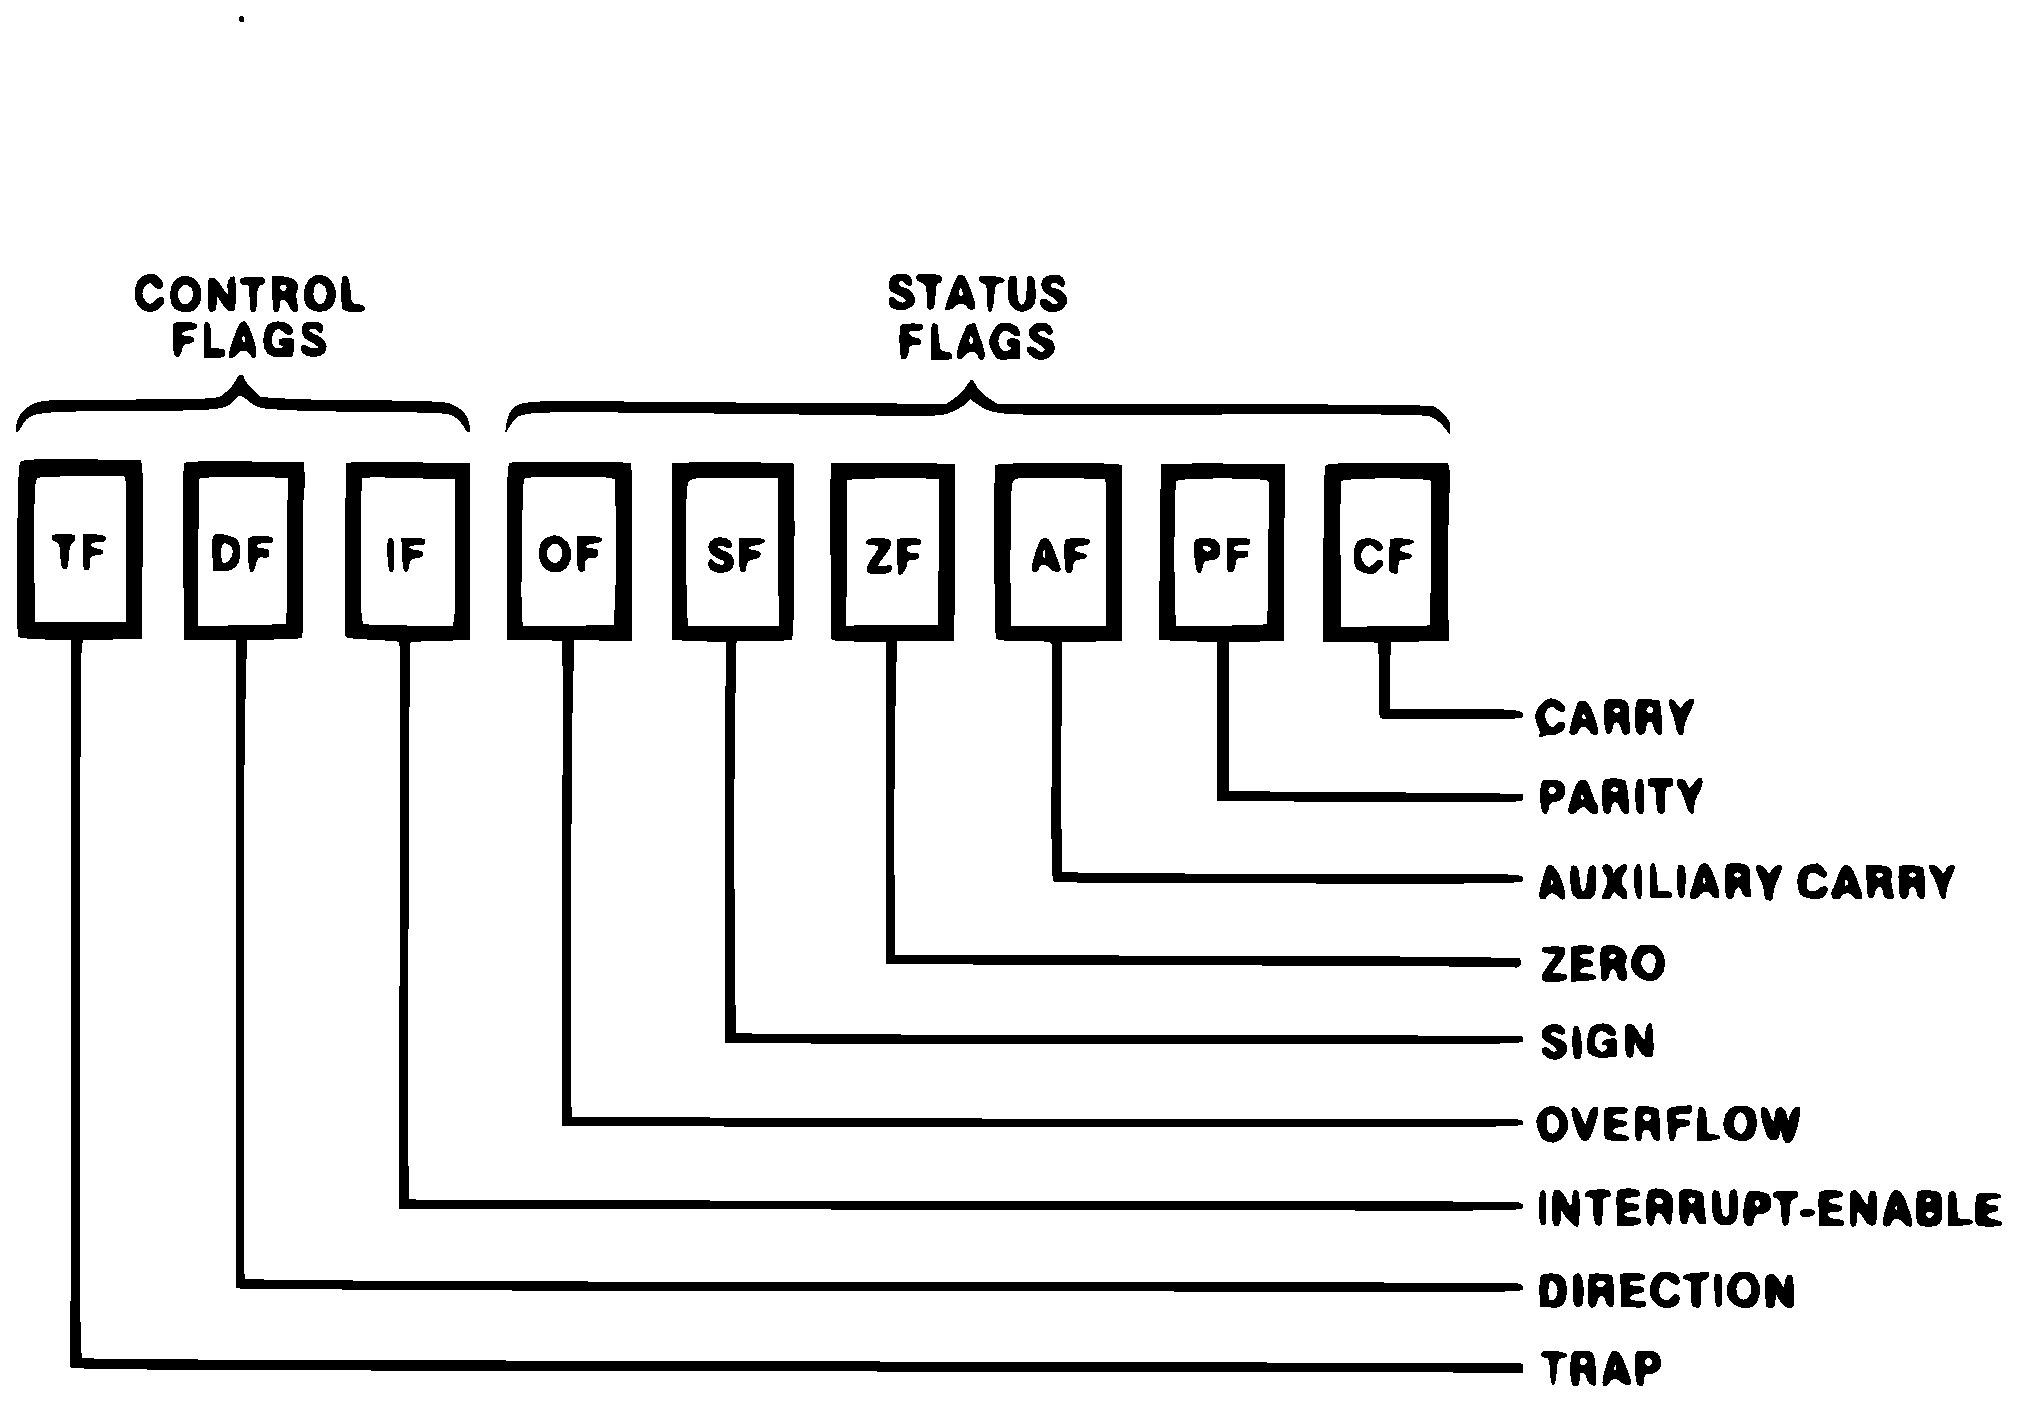
\includegraphics[scale=0.25]{figures/8086flags.eps}
  \caption{Flags}
  \label{fig:8086flag}
  \end{subfigure}
 \caption{8086 registers \cite{intel1979the}}
\end{figure}
The stack pointer register, \verb|sp|, and the base pointer register, \verb|bp|, are used for setting up stack frames and for accessing parameters passed to the functions. The source index register, \verb|si|, and the destination index register, \verb|di|, are used to provide the index of a single byte (or word) of source and destination strings, respectively.\\
\verb|bx| and \verb|bp| are used to provide the base address of a data structure or the stack frame. \verb|si| and \verb|di| are used to index through these data structures.\\
Segment registers are the "hack" which allow programmers to access 1 MiB of memory instead of mere 64 kiB. There are four 16-bit segment registers which are available to the BIU: code segment (\verb|cs|), data segment (\verb|ds|), extra segment (\verb|es|), and stack segment (\verb|ss|) registers (\autoref{fig:8086segr}). The purpose of segment registers is now presented.\\
A 16-bit register can address only 64 kiB of memory, with addresses of bytes going from 0x0000 to 0xffff (0 - 65535). If a 16-bit base value is left shifted by 4 bits and added to another 16-bit number, the resulting sum is a 20-bit number which can have any value in the range 0x00000 - 0xfffff (0 - 1048575). A 20-bit variable can address 1 MiB of memory. This is exactly how \textit{physical addresses} are generated from \textit{effective addresses}. In 8086, memory is divided in chunks, with the maximum size of chunks being 64 kiB. These chunks are called segments. The address at which a chunk starts is called segment base address. Segment base addresses are right-shifted by 4 bits and stored in segment registers. The effective address of a data or instruction byte is the offset at which that byte is located from the segment base address. Effective addresses can be stored in a general purpose register (in the case of data) or in the 16-bit instruction pointer, \verb|ip| (in the case of an instruction). To access the given data/instruction in a block, the BIU left-shifts the value stored in the segment register by 4 bits and to it adds the 16-bit effective address. The resulting 20-bit number is the physical address of the required data or instruction byte. The following relations will clarify the process of physical address generation.
\begin{enumerate}
  \item physical address of an instruction = (\verb|cs| $<<$ 4) + \verb|ip|
  \item \begin{enumerate}
    \item[a.] Byte or word in source string = (\texttt{ds} $<<$ 4) + \texttt{si}
    \item[b.] Byte or word in destination string =  (\texttt{es} $<<$ 4) + \texttt{di}
  \end{enumerate}
  \item physical address of a data byte = (\verb|ds|/\verb|es| $<<$ 4) + base address (\verb|bx|/\verb|bp|)\\
  \hspace*{8.7cm} + index (\verb|si|/\verb|di|)\\ 
  \hspace*{8.7cm} + diplacement (8-bit or 16-bit)
  \item address of the base of a stack frame = (\verb|ss| $<<$ 4) + \verb|bp|
  \item address of the top of a stack frame = (\verb|ss| $<<$ 4) + \verb|sp|
\end{enumerate}
As the value of lower nibble of the 20-bit segment base address is always zero, therefore, two segments have at least a gap of 16 bytes between them.\\
Besides the general purpose registers, the EU is also provided with a flag register having status and control flags (\autoref{fig:8086flag}). Status flags contain the represent the state of the machine after last operation (overflow, parity, carry bits, etc.). Control flag alter the way programs are executed by (direction of increment of index registers, interrupts, and single-step mode).

\subsubsection{Endianness}
The order in which a processor stores the high byte and low byte of a word is called \textit{endianness}. There are two types of endianness: little endianness and big endianness. If a processor stores the least significant byte at a lower address and most significant byte at higher address, then it is said to follow little-endian byte ordering. if a processor stores the most significant byte at a lower address and least significant byte at higher address, then it is said to be using big-endian byte ordering. 8086 follows little-endian byte-ordering. It should be noted that little-endian ordering is not applicable for values stored in registers. Therefore, if register \verb|ax| stores the number 0x1234, then \verb|al| will be storing 0x34 and \verb|ah| will be storing 0x12. On the other hand, if a memory location, say 0x1000 is said to store 0x1234, then 0x34 will stored at the address 0x1000, and 0x12 will be stored at the address 0x1001 (\autoref{fig:littlendian}).
\begin{figure}[h]
  \centering
  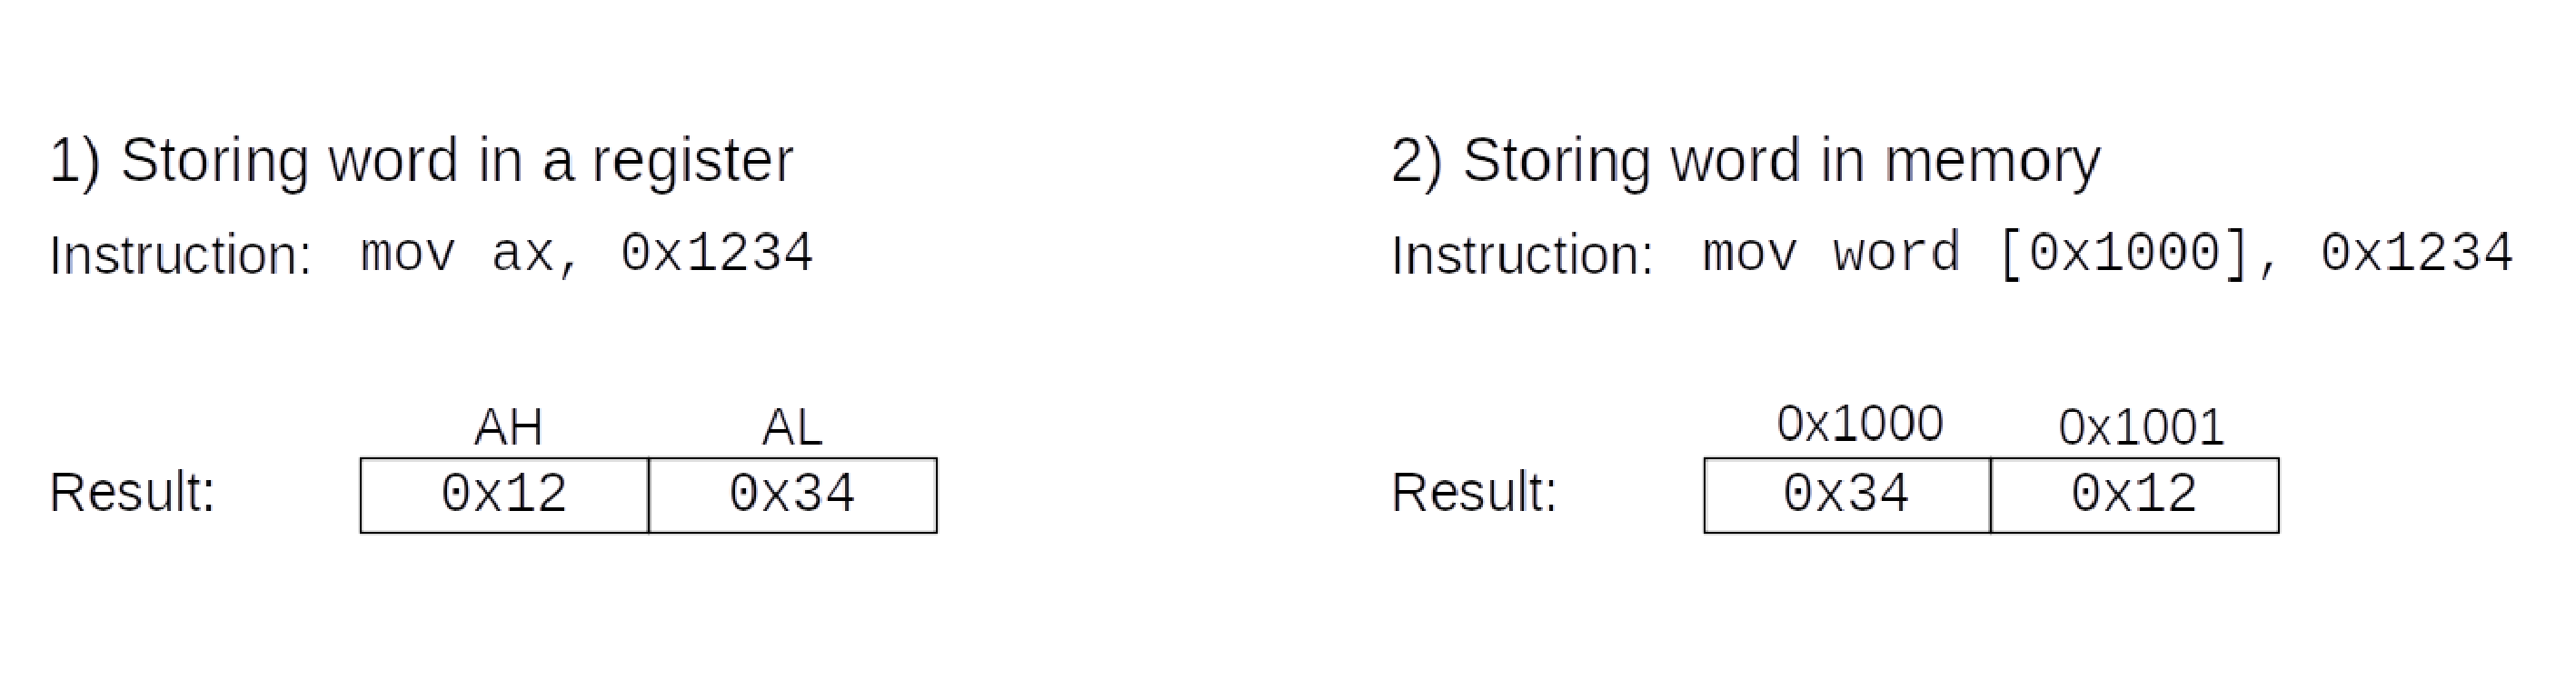
\includegraphics[scale=0.25]{figures/wordendian.eps}
  \caption{Ordering of bytes of words in registers and memory}
\label{fig:littlendian}
\end{figure}
Another type of data variable is a doubleword. A doubleword, as the name suggests, consists of two words and is used to store memory addresses. Therefore, it is often called as a pointer. As has already been discussed in section 2.4.3, physical address is made up of segment base address and an offset value. A doubleword's most significant word contains the segment base address, and its least significant word contains the offset of the data/instruction to be accessed. A doubleword is stored in memory by storing the least significant word (which contains the offset) at the lower address, and then storing the most significant word (which contains the segment base address) (\autoref{fig:doublewords}).
\begin{figure}[h]
  \centering
  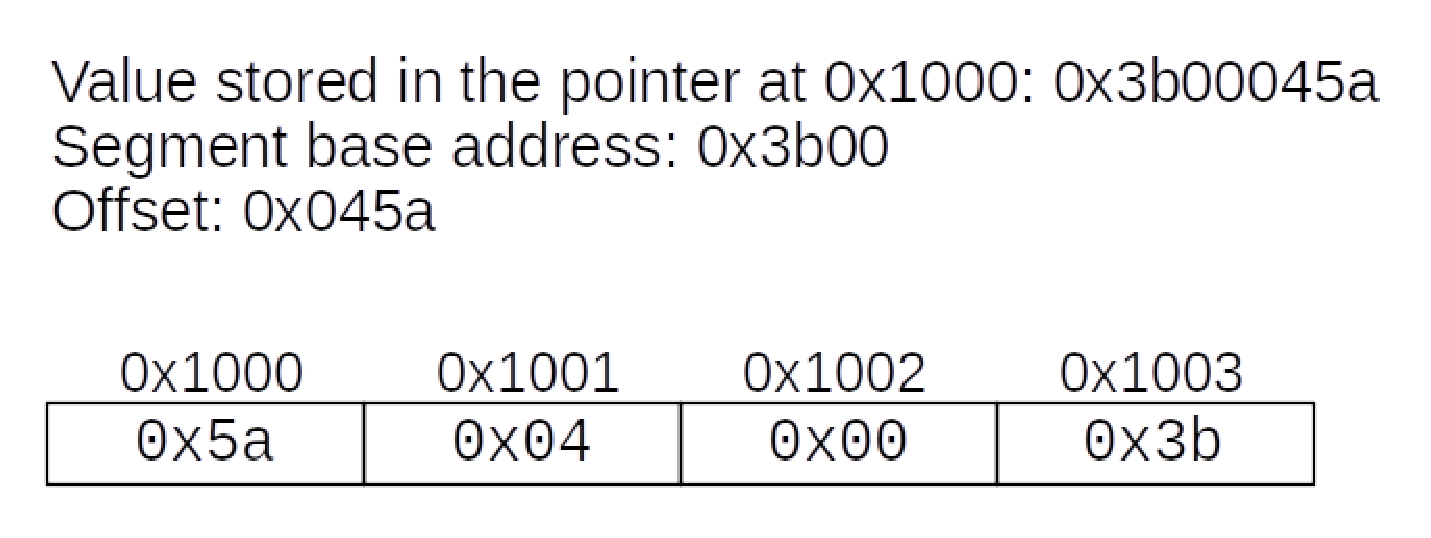
\includegraphics[scale=0.25]{figures/doublewords.eps}
  \caption{Storing doublewords in memory}
\label{fig:doublewords}
\end{figure}
This storing convention is most often used in intersegment calls where the calle's segment base address are first pushed onto the stack and the offset is pushed afterwards. After this, the far call instruction is executed, which pushes the current \verb|cs|'s and then \verb|ip|'s value onto the stack This is shown in \autoref{fig:stackops}. From the figure note that the stack grows downwards towards the base address of the segment in which the stack is kept.
\begin{figure}[h]
  \centering
  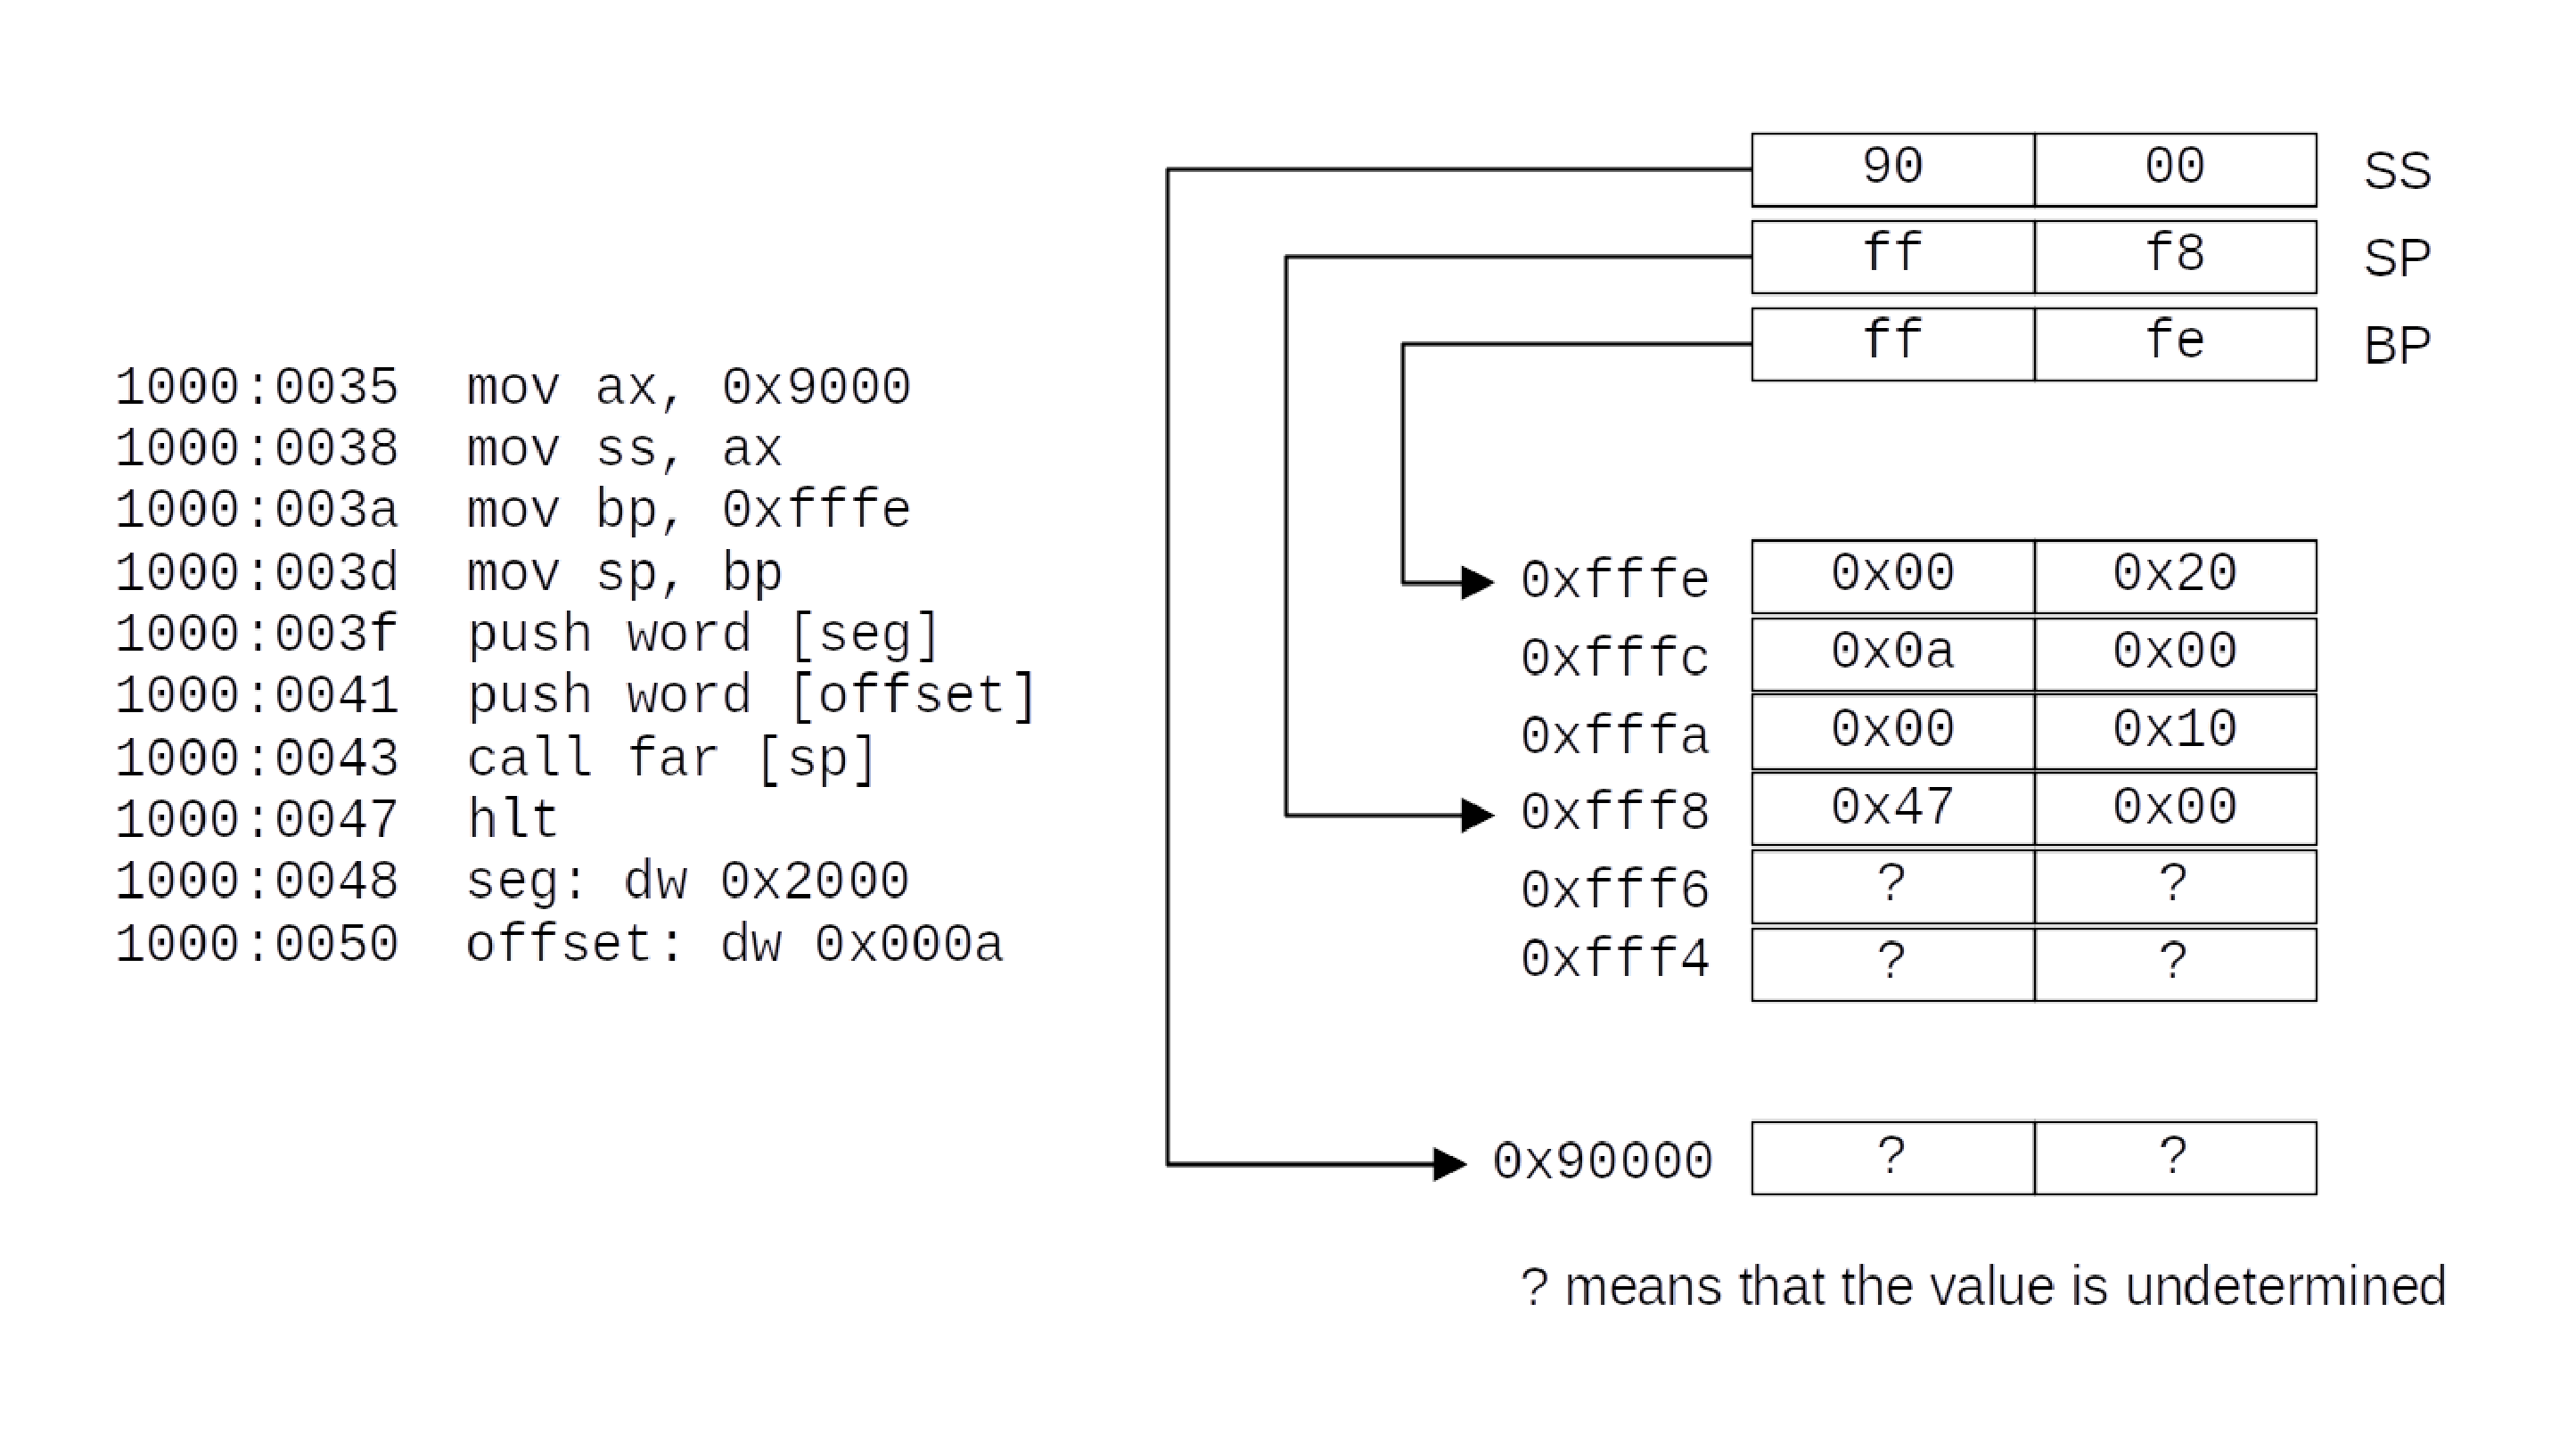
\includegraphics[scale=0.25]{figures/stackop.eps}
  \caption{Storing pointers on stack during intersegment calls}
\label{fig:stackops}
\end{figure}

\subsubsection{Addressing Modes}
Programming in 8086 assembly language is easier and enjoyable in comparison to programming in 8085's (or earlier microprocessor's) assembly language. This is because of the availability of powerful arithmetic, loop and string instructions, as well as the presence of different types of addressing modes. The addressing modes of 8086 are given below:
\begin{enumerate}
  \item \textit{Immediate Addressing}: Operand is provided in the instruction itself.\\Example: \verb|mov ax, 0x1234|.
  \item \textit{Register Addressing}: Both the operands are registers. Example: \verb|xor cx, cx|.
  \item \textit{Direct Addressing}: Effective address is provided in the instruction itself.\\Example: \verb|add ax, word [var1]|.
  \item \textit{Register Indirect Addressing}: The effective address is stored in base registers (\verb|bx| and \verb|bp|) or index registers (\verb|si| and \verb|di|). Example: \verb|mov al, byte [si]|. 
  \item \textit{Based Addressing}: The effective address used in the instruction is the sum of the value stored in a base register and a displacement. Using \verb|bp| as the base register allows us to access parameters of a function. Using \verb|bx| as the base register allows us to access data in a structure. Example: \verb|mov ax, word [bp + 2]|.
  \item \textit{Indexed Addressing}: Effective address is calculated from the sum of displacement and the value stored in one of the index registers. This is useful for accessing elements of an array. Example: \verb|mov dl, byte [si]|.
  \item \textit{Based Indexed Addressing}: The effective address is computed by adding a displacement, the value stored in a base register, and an index register. This addressing mode is useful in accessing elements of a parameter which might be a data structure. Example: \verb|mov dl, byte [bp + si + 4]|.
  \item \textit{String Addressing}: String instructions involve the use of string registers (\verb|si| and \verb|di|) and instructions. When string instructions are executed, it is assumed that \verb|si| is a pointer to the first byte or word of the source string, and \verb|di| is a pointer to the first byte or word of the destination string. Either \verb|si|, or \verb|di|, or both are either incremented or decremented depending on whether the direction flag is cleared or set, respectively. Example: \verb|repne lodsb|.
  \item \textit{I/O Port Addressing}: Peripherals which have port addresses are accessed using \texttt{in} and \verb|out| instructions. In direct port addressing, the 8-bit port address is provided with the instruction itself. The value being read or written is contained in \verb|al|. In indirect port addressing, the 16-bit port address is present in the register \texttt{dx}. Example: \verb|out 0x70, al|.
\end{enumerate}

\subsection{Design of the original IBM PC}
The original IBM PC was released on August 12, 1981. Thanks to its cheaper price, easily available hardware and software, and marketing, the IBM PC standardised the personal computer market. Although IBM no longer manufactures PCs, the IBM PC and its successors are still the \textit{de facto} standard for PCs \cite{ibmarchpc}.

\subsubsection{Physical Specifications}
Due its lower price and IBM's familiarity with it, the original IBM PC contained the 8088 microprocessor with a clock rate of 4.77 MHz. Clones of the IBM PC were released less than an year later, and some of them, like the Amstrad PC1512, had the 8086 microprocessor.\\
Both 8088 and 8086 can access 1 MiB of memory. However, as this memory was fairly large and expensive in the early 1980s, most PCs came with 16 kiB to 640 kiB of memory. Expansion slots were often provided for the user to increase the memory of the system themselves.\\
The original IBM PC came with upto two 5.25'' 160 kiB floppy disk drives. A disk-drive adapter was provided to interface with the disk drives. Cassette tape recorder and hard disks were also supported. Later versions of the IBM PC came with hard disk drives.\\
Addressing of storage disks was done using cylinder-head-sector (CHS) addressing. A single disk or a platter, in general, has two readable sides. A pair of heads were used to read and write to the disk. A single side of the disk was divided into tracks. A single track is contained within two concentric hollow cylinders and is made up of sectors, with each sector having 512 bytes of memory (\autoref{fig:chs}). Numbering of sectors start from 1, but the numbering of cylinders and heads starts from zero. The equation given below gives us the total size of the disk.
\begin{center}
$M = M_s \times N_s \times N_t \times N_h$
\end{center}
where
\begin{center}\begin{tabular}{ccl}\
$M$ &= &total storage capacity of the disk\\
$M_s$ &= &storage capacity of a single sector\\
$N_s$ &= &total number of sectors per track\\
$N_t$ &= &total number of tracks per head\\
$N_h$ &= &total number of heads per disk\\ 
\end{tabular}\end{center}
Consider the case of a standard 3.5'' floppy disk. It has the following specifications:
\begin{center}\begin{tabular}{ccl}\
$M_s$ &= &512 bytes/sector\\
$N_s$ &= &18 sectors/track\\
$N_t$ &= &80 tracks/head\\
$N_h$ &= &2 heads/disk\\ 
\end{tabular}\end{center}
which gives us
\begin{center}\begin{tabular}{ccl}
$M$ &= &$512 \times 18 \times 80 \times 2$\\
 &= &1474560 bytes\\
 &= &1.44 MiB
\end{tabular}\end{center}
Modern operating systems frequently  use logical block addressing (LBA) instead of CHS.\\
\begin{figure}[h]
  \centering
  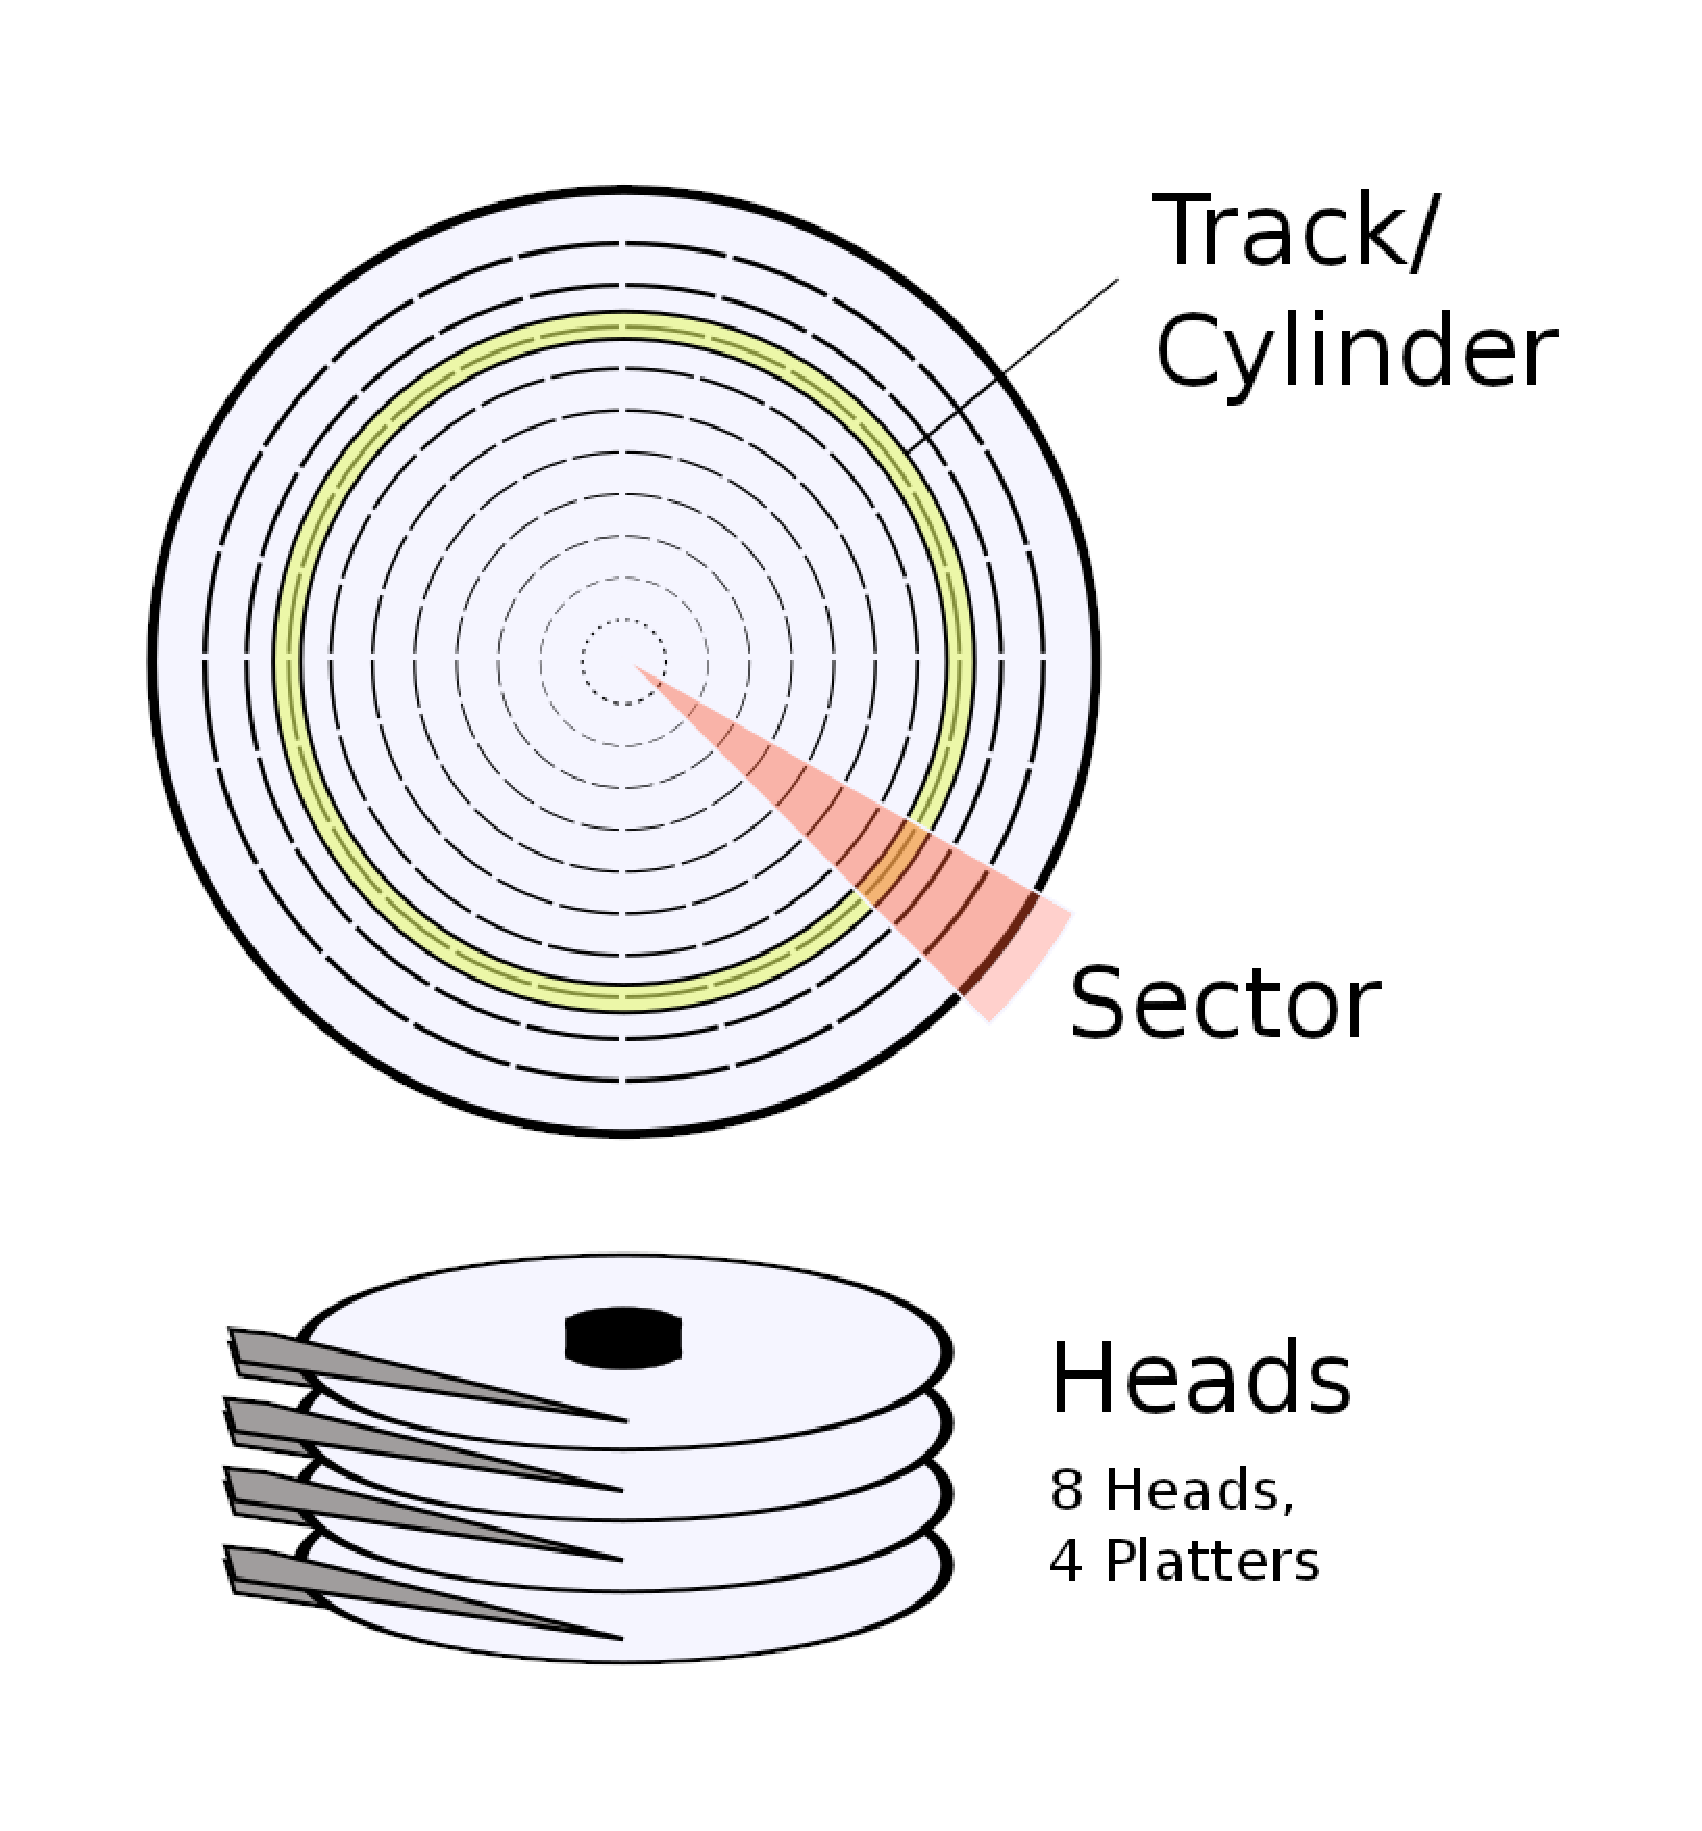
\includegraphics[scale=0.25]{figures/chs.eps}
  \caption{Cylinder/tracks, sectors and heads on a hard disk platter \cite{chsdiag}}
\label{fig:chs}
\end{figure}
For input, a standard IBM model F keyboard with 83 keys and five-pin connector was provided. The keys pressed on the keyboard were mapped to the characters present in the ROM of the CGA card. The characters present in the ROM were printable ASCII characters, diacritics, some Greek letters, and a few graphic characters. This character set present in the ROM was called IBM437 or "code page 437". Later models of IBM PC were shipped with VGA cards which supported a resolution of 640x480 pixels and had a 16-bit color palette.\\
To generate sounds, an 8254 programmable interval timer was used to generate square waves which were fed into a piezoelectric speaker.

\subsubsection{BIOS}
The term BIOS, standing for Basic I/O System, was coined by Gary Kildall. It is the firmware which is responsible for loading the bootloader from storage into the main memory. BIOS is stored in ROM and is the first software which is read by the CPU. Besides being responsible for loading the bootloader, the BIOS also provides the bootloader and real-mode OSs with several basic subroutines\footnote[1]{The words "procedure", "subroutine", and "function" have the same meaning and are used inter-changeably throughout this report.} which allow them to access the hardware.  These subroutines are called BIOS interrupts. BIOS interrupts are called by initializing the registers with appropriate values and issuing a software interrupt using \verb|int| instruction. For example, to print a character on the screen, BIOS interrupt 10,0E\footnote[1]{BIOS calls are mentioned in this report using INT N,F format. Here, N is the BIOS call number in hex-format, and F is the service which is required. F is usually an 8-bit number stored in \texttt{ah} before INT N is executed.} is used. To use this interrupt, 0x0e is stored in \texttt{ah} and the hex-code (from code page 437) of the character to be printed is stored in \texttt{al}. Then a software interrupt with interrupt number 0x10 is issued. The processor executes the ISR corresponding to interrupt 0x10 with \texttt{ah} = 0x0e in the BIOS and prints the character in \texttt{al} on the screen.\\
The BIOS in the original IBM PC was reverse engineered and cloned by other manufacturers so as to make their PCs compatible with the IBM PC. BIOS is slowly fading out of use in favour of UEFI. This is mainly because it is unsecure and is not supported in protected (32-bit) and long (64-bit) mode. \textit{Ralph Brown's Interrupt List} provides hobbyists and professionals with a comprehensive list of BIOS interrupts \cite{ralphintlist}.

\subsubsection{Boot Process}
When an IBM PC compatible computer is powered on or if the reset button is pressed, the BIOS performs a system check which is called power-on self-test (POST). POST involves initialization the main memory (RAM) and few important peripherals (e.g., keyboard, screen, speakers, disk drivers). If there is any error during POST, the BIOS informs the user about the same by generating beep codes from the speaker. Once the POST has been successfully completed, INT 19h is used to detect and load the bootloader from a bootable disk. A disk is considered to be bootable if the last word of its very first sector (track = 0 and head = 0) contains the magic number 0xaa55. As this sector also contains the bootloader, it is also known as boot sector or master boot record (MBR). Upon detecting the disk to be bootable, the BIOS loads the content of the MBR at address 0x7c00. The IP jumps to this address and CPU starts executing the instructions which make up the MBR. The bootloader might be simple enough to be contained in 512 bytes, or it might be complicated enough to be contained two sectors. In the latter scenario a two-stage bootloader is used. The boot sector code loads more sectors, and once the bootloader has been loaded, the kernel and then the operating system is loaded into the memory using BIOS calls.
\begin{figure}[h]
  \centering
  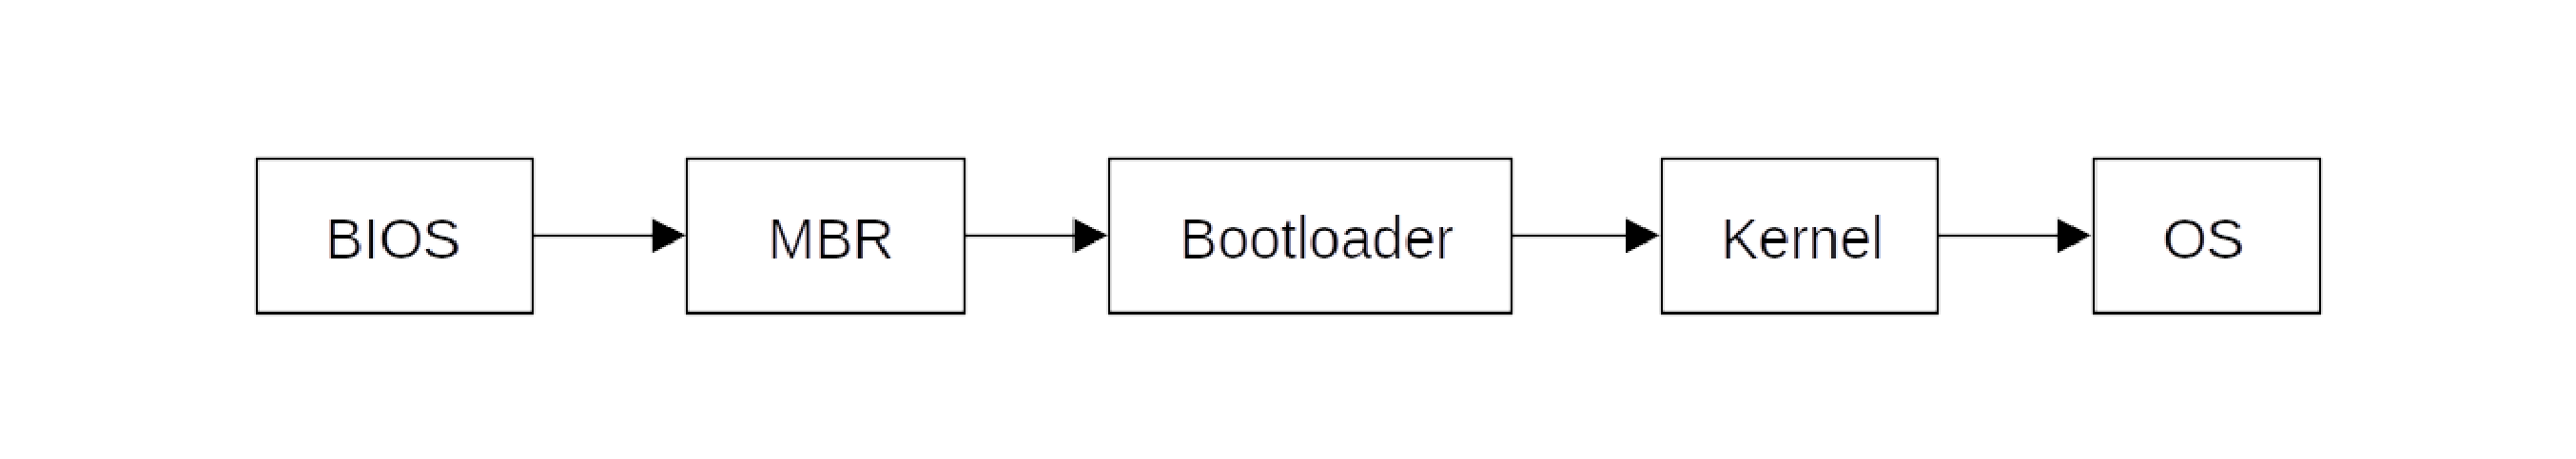
\includegraphics[scale=0.25]{figures/Booting.eps}
  \caption{Boot sequence of an IBM PC}
\label{fig:booting}
\end{figure}

\subsubsection{Memory Map}
Memory map is a diagrammatic/tabular method of showing the contents of physical memory of a computer system. In the case of the IBM PC, we are mainly interested in the memory map after booting has been completed. Therefore, by the term memory map we specifically mean the contents of memory after boot-up sequence.\\
The memory map is shown in \autoref{fig:memmap}. 

\begin{figure}[h]
  \centering
  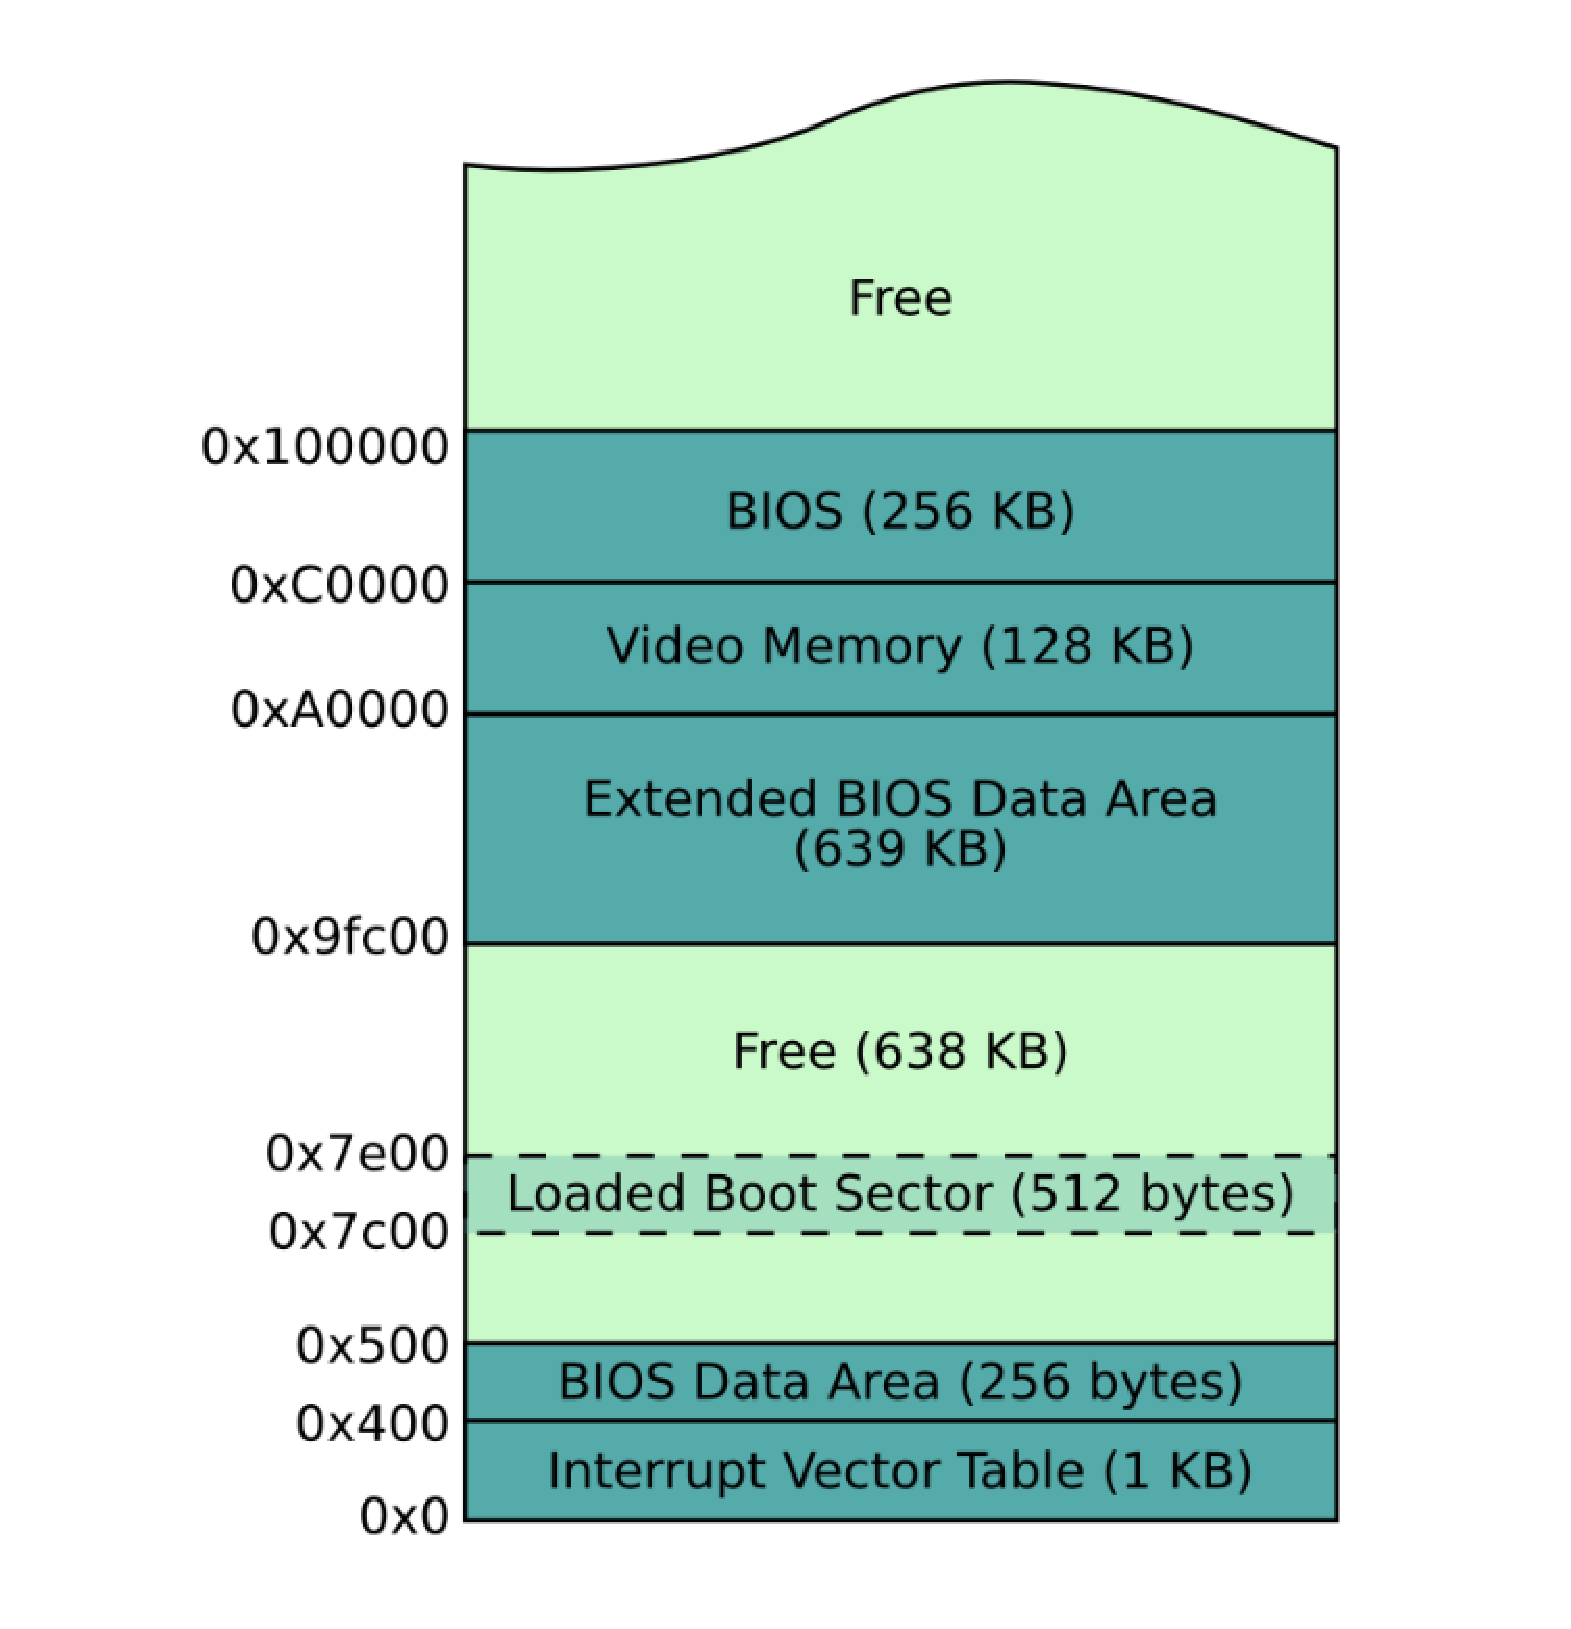
\includegraphics[scale=0.30]{figures/memmap.eps}
  \caption{Typical memory map of an IBM PC after boot \cite{blundell2009writing}}
\label{fig:memmap}
\end{figure}

As has already been discussed, the maximum size of a segment in 8086 is 64 kiB. Total addressable physical memory is 1 MiB. This memory is divided into continuous 64 kiB segments. Each of these segments is called a block. The blocks are differentiated from each other by the value of the most significant nibble of their segment base address. A block have segment base address equal to 0xn0000 is called block n. For example, the block starting at address 0x50000 is called block 5. Block 0 to block 9 make up 640 kiB of memory and together make up the \textit{low memory area} or \textit{conventional memory area} (LMA). Block A till F make up the \textit{upper memory area} (UMA) which has a size of 384 kiB. The blocks and the purpose they are usually used for is presented in \autoref{table:memmap}. Note that the blocks extended BIOS data area (EBDA) occupies varies from system to system and is, therefore, not mentioned in the table. However, EBDA is generally placed before block A.


\begin{table}[H]
\begin{center}
{\normalsize%
\caption{Typical Memory Map of an IBM PC after boot-up sequence}\label{table:memmap}
\begin{tabular}[t]{|c|c|c|c|}
\hline
\textbf{Block} & \textbf{Start} & \textbf{End} & \textbf{Description}\\
\hline
 & 0x000 & 0x3ff & Interrupt vector table (IVT)\\
	\cline{2-4}
  & 0x400 & 0x4ff & BIOS data area (BDA)\\
	\cline{2-4}
0  & 0x500 & 0x7bff & User memory\\
	\cline{2-4}
  & 0x7c00 & 0x7dff & Bootloader\\
	\cline{2-4}
  & 0x7e00 & 0xffff &\\
	\cline{1-3}
1 & 0x10000 & 0x1ffff &\\
	\cline{1-3}
2 & 0x20000 & 0x2ffff &\\
	\cline{1-3}
3 & 0x30000 & 0x3ffff &\\
	\cline{1-3}
4 & 0x40000 & 0x4ffff &\\
	\cline{1-3}
5 & 0x50000 & 0x5ffff & User memory\\
	\cline{1-3}
6 & 0x60000 & 0x6ffff &\\
	\cline{1-3}
7 & 0x70000 & 0x7ffff &\\
	\cline{1-3}
8 & 0x80000 & 0x8ffff &\\
	\cline{1-3}
9 & 0x90000 & 0x9ffff &\\
\hline
A & 0xa0000 & 0xaffff & Video memory\\
	\cline{1-3}
B & 0xb0000 & 0xbffff &\\
\hline
C & 0xc0000 & 0xcffff &\\
	\cline{1-3}
D & 0xd0000 & 0xdffff & Mapped to ROM and hardware\\
	\cline{1-3}
E & 0xe0000 & 0xeffff &\\
	\cline{1-3}
F & 0xf0000 & 0xfffff &\\
\hline
\end{tabular}}
\end{center}
\end{table}


\subsection{Deficiencies of Model Curriculum for Engineering and Technology Developed by AICTE}
We discussed in section 1.1 on how engineering is a practical profession which necessitates that engineering students should have practical knowledge of the field they establish their career in. With the aim of getting students employed in an ever-changing industry, it becomes increasingly hard to keep the syllabi appropriately updated. Neither the institutions responsible for maintaining and enforcing the curriculum, nor the students can be entirely blamed for the lack of practical knowledge which can be found among many freshers across the globe. A discussion of the global technical education scenario would increase the length of the present chapter which is already beyond the usual length. Therefore, we will restrict our discussion to the brief analysis of engineering education in India. This will be appropriate as:
\begin{enumerate}
\item All the authors of this report bear the nationality of Indian.
\item It is estimated that India will be the leading producers of engineers by the end of the current and the coming decades \cite{ind2015eng}. This makes it important that the quality of engineers being produced is great.
\end{enumerate}
It is a well known fact that engineering education in India is not at par with the requirements of the industry. This fact has been pointed out by many people over the years, more recently by Steve Wozniak who pointed out that innovation has taken a backseat in pursuit of employability \cite{woz2018eng}. Such criticism often results in a blame game. Sometimes counterarguments also blame the British rule. The fact that after more than half a century of independence, we, as a nation, have failed to nurture and promote original thinking and creativity is disregarded. The number of jobs related to computer science and IT are ever increasing. Students in pursuit of getting employed often curb their interests and enrol in courses related to computer science and IT \cite{popengtoi}. Innovation and practicality go hand in hand. The saying "\textit{Necessity is the mother of innovation}" is an adage to this. Without getting their hands dirty, a person can never know about the requirements of a particular field. Therefore, it becomes necessary to ensure that students are dispensed practical knowledge in as many areas as possible. By doing so, they can determine their interests and contribute to the fields they like. The best way to dispense practical knowledge is by incorporating project-based learning in the curriculum for technical education.\\
Though the model curriculum provided by the All India Council for Technical Education (AICTE) is developed with the help of academic and industry experts \cite{basu2018model}, they have some glaring flaws, three of which are stated below.
\begin{enumerate}
	\item \textit{Undirected and overloaded course structure}: A single course consists of many theoretical sub-topics without any practical problems for students to work through. A student can solve tons of problems on Kirchhoff's rules however their ability to synthesize a circuit is equally important. As the project presented in this report is related to computer architecture and operating systems, we will take the example the course on Computer Architecture offered to Electrical Engineering undergrads. There are six modules in this course. Module 1 tells about the differences between CISC and RISC, data types, system buses, and multi-bus organization. Module 2 then jumps to memory organization, followed by Module 3 discussing I/O devices, PCI and PCI Express bus. Module 4 then discusses x86 architecture, and its addressing modes and instruction. Module 5 discusses instruction level pipelining (ILP) and module 6 discusses other architectures like MIPS. The course, and other similar courses, can be considered to be well designed theoretically. However, they are overloaded with theoretical concepts. It would be better to just focus on the architecture of single computer, preferably IBM PC. The course can then describe the 8086 microprocessor and later describe ILP, and paging. Then the architecture of the IBM PC can be dealt with in detail.
	\item \textit{Impractical course structure}: Continuing with the example provided previously, most of the courses dealing with microprocessors start of with 8085 microprocessor. Though it is still used in legacy systems in the industry, no new projects are developed using it. Students would be better served by teaching them about ARM or RISC-V or x86 architectures as most of the computing systems today are built around them. Furthermore, it must be noted that the practical assignments given to students are trivial. Examples include writing subroutines to multiply numbers, or to move strings in 8086's assembly language. A more practical exercise would be to write subroutines to print a string on the screen or to separate words out from a string.   
	\item \textit{Obsolete software tools}: Most of the software tools used in colleges are obsolete. Courses on C programming and data structures still require students to develop and run code in Turbo C environment. This is ridiculous because Turbo C's compiler does not follow the standard implementation of C and C++. In the course on microprocessors, codes are run on expensive trainer kits or on emulators, like emu8086, which is not the industry standard for developing 8086 assembly code.
\end{enumerate}
Remedying the current problems will take years. However, one should not be daunted by this challenge. Baby-steps are what is required. The project presented in this report is one such baby-step. It is hoped that it will assist in nurturing students who are interested in computer architecture and they will not have to face the problems which the author of this project (Kapoor) had to face.



\section{Objective}
The objective of this project was to develop a simple real mode operating system from scratch for educational purposes. This was objective was achieved by completing the following sub-objectives:
\begin{enumerate}
\item To develop a bootloader from scratch.
\item To develop a set of libraries containing certain standard functions found in C's \verb|stdio.h| and \verb|string.h| libraries. This would assist the user in building disk applications for the system.
\item To develop a shell which enables the user to issue basic commands to interact with system components like disks, APM, etc.
\item To develop a file system using contiguous sector allocation. The file system should be simple enough to understand, implement and use with programs like the line editor.
\item To develop a build environment which allows the user to write and build their own disk applications, and run them using the operating system.
\end{enumerate}

\section{Overview}
In the present chapter we discussed about our motivation behind developing a simple operating system. In chapter 2 we discuss the implementation of CrazyOS. We have explained the source tree of the parent and the project directory along with the library functions.\\
In Chapter 3, we have provided the results of this project. Screenshots of the operating system running on an emulator are presented to the reader. The only three known bugs in the operating system are also discussed.\\
In Chapter 4, we have given a few concluding remarks and have discussed the future scope of this project.\\
The report ends with the presentation of the references, research paper, and resume of the authors.        
%%%%%%%%%%%%%%%%%%%%%%%%%%%%%%%%%%%%%%%%%%%%%%%%%%%%%%%%%%%%%%%%%%
%%%%%%%%%%%%%%%%%%%%%%%%%%%%%%%%%%%%%%%%%%%%%%%%%%%%%%%%%%%%%%%
\newpage
\chapter{\centering Implementation of CrazyOS}

\section{Introduction}
In the previous chapter we discussed our motivations behind creating a very basic operating system, CrazyOS. We described it as a single-user, single-tasking, real mode operating system. These three terms are described as follows:
\begin{enumerate}
  \item \textit{Single-user}: Most modern operating systems allow multiple user accounts. Each user has some disk space allocated to them and they can use it as they like. They can keep their personal files and projects separate from others work. Each user account is accessible through a password. CrazyOS does not support multiple users. It does not have the capability to communicate through a network with other computers. It is intended for one user only. No password logins are required to access the services of the system or to access the contents of a file.
  \item \textit{Single-tasking}: Modern operating systems allow users to run multiple programs at once. Each program is given its own address space to run without messing with other programs. Various scheduling algorithms, for example round-robin scheduling algorithm, are used to allocate a quantum of CPU's time to programs so that each program gets executed and give the user a feel of simultaneous execution of multiple programs. Threads and cores are also allocated to different batches of programs. CrazyOS is simple: it runs on a single processor and only a single program/process, which is the shell, is running most of the time. Other programs can be run either by passing commands from the shell, or by loading and running them from the disk.
  \item \textit{Real mode}: Modern operating systems run on 64-bit CPUs. One such CPU is the x86-64 family of processors produced by both AMD and Intel. These processors use 64-bit registers and address space and use paging (i.e., creation of virtual address spaces) to protect programs from each other. To provide backwards compatibility to programs which would run only on 32-bit and 16-bit machines, x86-64 processors initially run as 16-bit processors when the machine has just been powered on. In this mode, they try to act like an 8086 processor. This mode of operation is called \textit{real mode} or \textit{virtual 8086 mode}. After going through a complex setup procedure, the user can use the processor in 32-bit mode which is called \textit{protected mode}. After some more setting up, the user can finally run the processor in 64-bit or \textit{long mode}. In this mode, programs can utilize all the capabilities of the processor. Most modern operating systems run in long mode. However, to reduce complexity of its design and to make it relevant for use as a tool in courses on computer architecture and 8086 microprocessor, CrazyOS runs in real mode or virtual 8086 mode only.   
\end{enumerate}
The implementation of CrazyOS is presented in this chapter. We will begin by describing the build environment and organization of the source files. Integral components of the operating system are then discussed in detail.

\section{Set-up of the Development Environment}
The development environment of CrazyOS consists of five software tools: code editor, assembler, emulator, build automation software, and source version control software. We will now explain the tools of choice for this project.

\subsection{Code Editor}
Earlier versions of the operating system were written using gVim. As the size of the project grew, the author found it difficult to maintain files using gVim. Therefore, a switch to VScode was made and it has since become the default code editor for this project. \textit{x86 and x86\_64 Assembly} syntax highlighting extension was downloaded as it supported NASM's syntax. Github's dark theme is used as the author find it to be pleasing to his eyes.

\subsection{Assembler}
Many assemblers supporting the x86 architecture are available. The author had the choice of using either GNU AS or NASM. GNU AS is a part of GCC and supports multiple architectures. Due to this reason, it is used for developing and maintaining assembly source files in many projects such as the Linux kernel. However, it by default uses AT\&T syntax which is different from Intel syntax, the latter being found in datasheets and software developer's manuals provided by both AMD and Intel. Few of the differences between AT\&T and Intel syntax are listed below:
\begin{enumerate}
  \item Intel syntax requires that after writing the instruction, the user has to first mention the destination operand and then the source operand. AT\&T syntax requires that the source operand is to be mentioned first. Therefore, \texttt{mov eax, ebx}, written in Intel syntax, and \texttt{movl \%ebx, \%eax}, written in AT\&T syntax, are both equivalent to each other.
  \item Register names are prefixed with \verb|%|, immediate and static operands with \verb|$| and hexadecimal numbers are prefixed with \texttt{0x}.
  \item Size of the operands is to be mentioned by suffixing a literal(s) with the instruction mnemonic. Three most commonly used literals are \verb|b| for byte operands, \verb|w| for word operands, and \verb|l| for doubleword operands.  
\end{enumerate}
Therefore, \texttt{mov byte [bx], al}, written in Intel syntax, and \texttt{movb \%al, (\%bx)}, written in AT\&T syntax, are equivalent to each other. Being a beginner himself, the author found out that it takes sometime to get used to AT\&T syntax. Furthermore, GNU AS partially supports Intel syntax and its documentation was found to be bit terse at places. Therefore, the author decided to use the Netwide Assembler, or NASM as it is usually called, for assembling the source files. NASM supports only x86 and x86-64 architecture and by default uses Intel syntax. It has a rich set of preprocessor directives which make it easier to include files and write macros. It can output assembled files in many different formats, such as ELF, plain binary, COM, etc. An excellent documentation is also provided by the NASM development team \cite{nasm2015doc}.

\subsection{Emulator}
The author had a bad experience with emu8086 which is widely used in courses dealing with 8086 microprocessor in Indian colleges. The emulator comes with a free trial period of 14 days after which a license needs to be purchased. The emulator's free trial ended on the day of practical examination, which infuriated all of his colleagues including the author himself. He also found it to be impossible to link his own software with the emulator, which the documentation stated was possible.\\
During the development of CrazyOS, the author had the choice to either use VMware Workstation Player or QEMU. Both of these software are used by professionals for testing operating systems, with the former being a virtualization software and the latter being an emulator. A virtualization software allows the user to run a guest OS meant for the same architecture on which the host OS is running. Resources of the system are managed by the virtualization software, in this case VMware Workstation Player. In the case of an emulator, software fills in the role of hardware by emulating hardware devices. An emulator allows the user to run software which is meant for different architectures. QEMU uses kernel-based virtual machine which uses translation of guest machine's instructions to host machines at byte level, which allows it to run guest OS at near native speed \cite{bellard2005qemu}.\\
VMware Workstation Player was found to be using too many resources when running Windows XP on the author's laptop. It was also found that it was not able to boot CrazyOS properly. As the author found QEMU to be able to run Windows XP and toy operating systems with ease on his machine, he chose it over VMware Workstation Player and has used it for testing CrazyOS. In particular, QEMU's emulation of an IBM PC using i386 (80386) microprocessor has been used for testing the operating system. This emulator is ran from the terminal using the command \verb|qemu-system-i386|. Emulation of various peripherals and disk drives can be connected to it using by specifying them with typing appropriate commands after typing the name of machine to be emulated. For example, if the user has a binary file, \verb|file.bin| which he wishes to use a floppy disk A for an i386 based IBM PC, he can do so by executing the following command:\\
\texttt{qemu-system-i386 -fda file.bin}

\subsection{Makefile}
GNU Make is widely used by developers across the globe for building object files and executables automatically without retyping commands for building each source file. The author has used a single makefile, \verb|CrazyOS/8086/Makefile|, for building the image of the operating system.

\subsection{Git}
Git is the most popular source version control software. It used for maintaining many big open source projects such as the Linux kernel and VScode. A local Git repository can be linked to a remote repository on the internet. Most developers use Github as the platform for hosting their projects and collaboratively developing and maintaining them. The author has used Git v2.34.1 for maintaining this project. The project is hosted at \url{https://github.com/PraneetKapoor2619/CrazyOS}, with the latest short commit ID as of writing this report being \href{https://github.com/PraneetKapoor2619/CrazyOS/tree/1a17fa09b6df15038edabdefe9fd9ab04cb80907}{1a17fa0}.   

\section{Structure of the Project Directory}
CrazyOS started out as a project to teach its author about the 8086 microprocessor and the IBM PC. The author expects to write similar toy operating systems for computers using i386, x86-64, ARM and RISC-V processors. These ambitions are reflected in the commit history and by the structure of the project directory. We will begin by explaining the structure of the parent directory, \verb|CrazyOS/|. The rest of this chapter and the report will be concerned with the contents of \verb|CrazyOS/8086/| directory.

\subsection{Parent Directory}
Assuming the reader clones the project from Github into a directory named \verb|CrazyOS|, the directory tree that will be obtained is shown in \autoref{fig:parentdirtree}. \textit{depth = 0} indicates the number of files and subfolders that are being shown in the source tree.\\

\begin{figure}[H]
\begin{forest}
  for tree={
    font=\ttfamily,
    grow'=0,
    child anchor=west,
    parent anchor=south,
    anchor=west,
    calign=first,
    edge path={
      \noexpand\path [draw, \forestoption{edge}]
      (!u.south west) +(7.5pt,0) |- node[fill,inner sep=1.25pt] {} (.child anchor)\forestoption{edge label};
    },
    before typesetting nodes={
      if n=1
        {insert before={[,phantom]}}
        {}
    },
    fit=band,
    before computing xy={l=15pt},
  }
[CrazyOS
  [8086]
  [cos]
  [Documentation]
  [.git]
  [LICENSE]
  [README.md]
  [.gitignore]
]
\end{forest}
\caption{Parent directory tree (depth = 0)}
\label{fig:parentdirtree}
\end{figure}

The reader will observe that there is a folder named \verb|8086|. It contains the source files for building 16-bit real mode version of CrazyOS which is the subject matter of this report. When in future the author develops CrazyOS for a computer using a processor other than 8086 (or x86-64 in real mode), the source file for that version of CrazyOS will be put in a folder bearing the name of the processor. For example, if the author releases CrazyOS for i386 based computer, its source files will be placed in a folder named \verb|i386|.\\
Restructured text (\verb|.rst|) files are used to write documentation in favour of markdown files. These files are kept in \verb|CrazyOS/Documentation/source/| folder. Documentation for different versions of CrazyOS will be kept in folders bearing the name of the processor for which the operating system is designed. Sphinx is the tool which is used for generating documentation using \verb|.rst| files. It can generate documentation in HTML, PDF, LaTex, etc. formats. The configurations for the Python environment using Sphinx is stored in \verb|CrazyOS/cos/| folder. The documentation so generated can be published online using \href{https://readthedocs.org/}{readthedocs.org}. This has been done by many project communities, for example, \href{https://docs.kernel.org/}{The Linux Kernel documentation} and \href{https://www.qemu.org/docs/master/}{QEMU's documentation} have been made and published using the aforementioned toolchain. It should be noted that the documentation for this project is still a work in progress.\\
Finally, we come to \texttt{LICENSE} and \texttt{README.md}. \texttt{LICENSE} file contains a copy of GNU/GPL Version 3 license under which the project is released. GNU/GPL is a \textit{"free, copyleft license for software and other kinds of works."}. As per this license, the project is distributed as a free software which can be modified by others. \texttt{README.md} contains a brief introductory text which tells the reader about the motivation and scope of the project. If the user has enabled the option to view hidden files and folders, he will observe that there is folder named \verb|.git| and a file named \verb|.gitignore| present in the parent directory. The former stores the Git configuration files for this directory/repository. The latter stores the extensions which should not be tracked by Git.\\

\subsection{Project Directory: ../8086}
As has been mentioned before, the directory \texttt{../8086}\footnote[1]{\texttt{..} is used to refer to the parent directory, in this case \texttt{CrazyOS}. In fact, \texttt{CrazyOS} is itself a part of some directory and therefore it can be written as \texttt{../CrazyOS}.\\} contains the source files for the project. The tree of this directory is given in \autoref{fig:dirtreecrazyos86}.\\
\begin{figure}
\begin{forest}
  for tree={
    font=\ttfamily,
    grow'=0,
    child anchor=west,
    parent anchor=south,
    anchor=west,
    calign=first,
    edge path={
      \noexpand\path [draw, \forestoption{edge}]
      (!u.south west) +(7.5pt,0) |- node[fill,inner sep=1.25pt] {} (.child anchor)\forestoption{edge label};
    },
    before typesetting nodes={
      if n=1
        {insert before={[,phantom]}}
        {}
    },
    fit=band,
    before computing xy={l=15pt},
  }
[CrazyOS/8086
  [apps]
  [boot]
  [build]
  [disk-apps]
  [include]
  [kernel]
  [.vscode]
  [Makefile]
  [mkdisk1.asm]
  [mkdisk2.asm]
  [README.md]
]
\end{forest}
\caption{Directory tree for \texttt{CrazyOS/8086} (depth = 0)}
\label{fig:dirtreecrazyos86}
\end{figure}
Except for \verb|.vscode| and \verb|README.md|, the files and folders in the source tree shown in \autoref{fig:dirtreecrazyos86} form the \textit{soul} of this project. They are discussed in following sections in the order in which they are executed when the operating system runs on the emulator. Before ending this section, we explain the purpose of \verb|.vscode| and \texttt{README.md}. \verb|.vscode| contains four files, namely \texttt{configurationCache.log}, \texttt{dryrun.log}, \texttt{settings.json}, and \texttt{targets.log}. These files setup the VScode environment (theme and syntax highlighting) which has been described in section 3.1.1. \texttt{README.md} is a project description file.
\section{Bootloader: ../boot}
The bootloader was the first program which was developed for this project. All the files which are related to it are kept in \texttt{../boot} directory.
\begin{figure}[H]
\begin{forest}
  for tree={
    font=\ttfamily,
    grow'=0,
    child anchor=west,
    parent anchor=south,
    anchor=west,
    calign=first,
    edge path={
      \noexpand\path [draw, \forestoption{edge}]
      (!u.south west) +(7.5pt,0) |- node[fill,inner sep=1.25pt] {} (.child anchor)\forestoption{edge label};
    },
    before typesetting nodes={
      if n=1
        {insert before={[,phantom]}}
        {}
    },
    fit=band,
    before computing xy={l=15pt},
  }
[CrazyOS/8086/boot
  [boot.asm]
  [boot\_util.asm]
]
\end{forest}
\caption{Directory tree for \texttt{CrazyOS/8086/boot} (depth = 0)}
\label{fig:dirtc8boot}
\end{figure}

As can be seen from \autoref{fig:dirtc8boot}, there are two files in \texttt{../boot}, namely, \texttt{boot.asm} and \texttt{boot\_util.asm}. We will now explain both of these files.

\subsection{boot.asm}
\texttt{boot.asm} is the main bootloader source file which is responsible for loading the kernel header from the storage disk. The storage disk in this project is the bootable floppy disk image,\\\texttt{../build/CrazyOS.bin}. Besides loading the kernel header, the bootloader is also reponsible for clearing the screen, setting background and foreground colors, and finally setting the page number and cursor position.\\
\texttt{boot.asm} begins with the following directives:
\begin{Verbatim}
cpu 386
bits 16
align 16

org 0x7c00
\end{Verbatim}
\texttt{cpu 386} directive tells NASM that the source code in the current file is written for a computer having i386 processor. \texttt{bits 16} directive tells the assembler that the instructions used in the source code are 16-bit instructions and not 32-bit instructions. Aligning data and instructions such that they start at even-numbered addresses allows the processor to easily access them which speeds up the execution speed \cite{intel1979the}. This requires aligning data and instructions by 16-bits, which is done using \texttt{align 16} directive. Finally, the directive \texttt{org 0x7c00} tells the assembler that the source file will be loaded at the address 0x7c00. Therefore, addresses of all instructions and data in the given source file should be calculated with respect to this base address.\\
Using \texttt{\%include "boot/boot\_util.asm"} we include the source code of \texttt{boot\_util.asm} in \verb|boot.asm| which allows us to use functions present in the included file. To jump around this portion of the code and run the main body of the bootloader, we use \texttt{jmp boot\_main}.\\
In the main body of the bootloader, we initialize the stack using the following instructions:
\begin{Verbatim}
boot_main:
	mov bp, 0x7ffe
	mov sp, bp
\end{Verbatim}
The base point \verb|bp| points at an even-address as this allows the process to perform stack operations faster. As nothing is currently present in the stack, the stack pointer points at the same address as the base pointer.\\
We now call \verb|clrscr|, \verb|reset_curse|, and \verb|set_pg| subroutines to clear the screen and set its colour, reset cursor position, and set the page number to 0, respectively. Colour of the screen is set by putting 0x1f in register \verb|bh| before executing INT 10,07 interrupt. The higher nibble stores the hex-code for background colour and the lower nibble stores the hex-code for the foreground colour. Different 8-bit colours and their hex-codes are given in \autoref{table:8bitcolour}.

\begin{table}
\begin{center}
{\normalsize%
\caption{Hex-codes for 8-bit colours}\label{table:8bitcolour}
\begin{tabular}[t]{|c|c|}
\hline
\textbf{Hex-code} & \textbf{Colour}\\
\hline
0 & Black\\
\hline
1 & Blue\\
\hline
2 & Green\\
\hline
3 & Cyan\\
\hline
4 & Red\\
\hline
5 & Magenta\\
\hline
6 & Brown\\
\hline
7 & Grey\\
\hline
8 & Dark grey\\
\hline
9 & Bright blue\\
\hline
a & Bright green\\
\hline
b & Bright cyan\\
\hline
c & Bright red\\
\hline
d & Bright Magenta\\
\hline
e & Yellow\\
\hline
f & White\\
\hline
\end{tabular}}
\end{center}
\end{table}

After these \textit{beautification} procedures, the operating system is loaded from disk by \texttt{read\_disk} subroutine. This subroutine uses INT 13,02 to read the disk. As of writing this report, the operating system has a size of 5.9 kiB which makes it necessary that more than one sector are loaded from disk. A total of 32 (0x20) sectors are read. The operating system is loaded at address 1000:0000. The disk operation is considered to be successful if INT 13,01 returns 0x00 in \verb|al|.\\
To actual run the operating system, we have to perform an intersegment jump to 1000:0000 where the kernel header has been loaded. This is done by pushing 0x1000 and 0x0000 to the stack and executing a far return instruction, \verb|retf|.\\
As has been mentioned in section 2.5.3, the first stage of the bootloader should be fit into the very first sector of the disk. The disk should also be bootable else the bootloader will never be loaded by the BIOS into the memory. To mark the disk as bootable, the magic number 0xaa55 is placed at the end of the bootsector. We do this by using the following directive:
\begin{Verbatim}
	times 510 - ($ - $$) db 0	
	dw 0xaa55		; magic number
\end{Verbatim}
A padding of zero is performed by \texttt{times} directive which repeats a null byte till the size of the bootloader is equal to 510 bytes. The magic number is then placed. This is shown in \autoref{fig:boothexdump} which shows the hexdump of the bootloader. As x86 family uses little-endian byte ordering, therefore, 0x55 is placed first and then 0xaa is placed. There occupy the 510th and 511th bytes of the bootsector, respectively.

\begin{figure}[h]
  \centering
  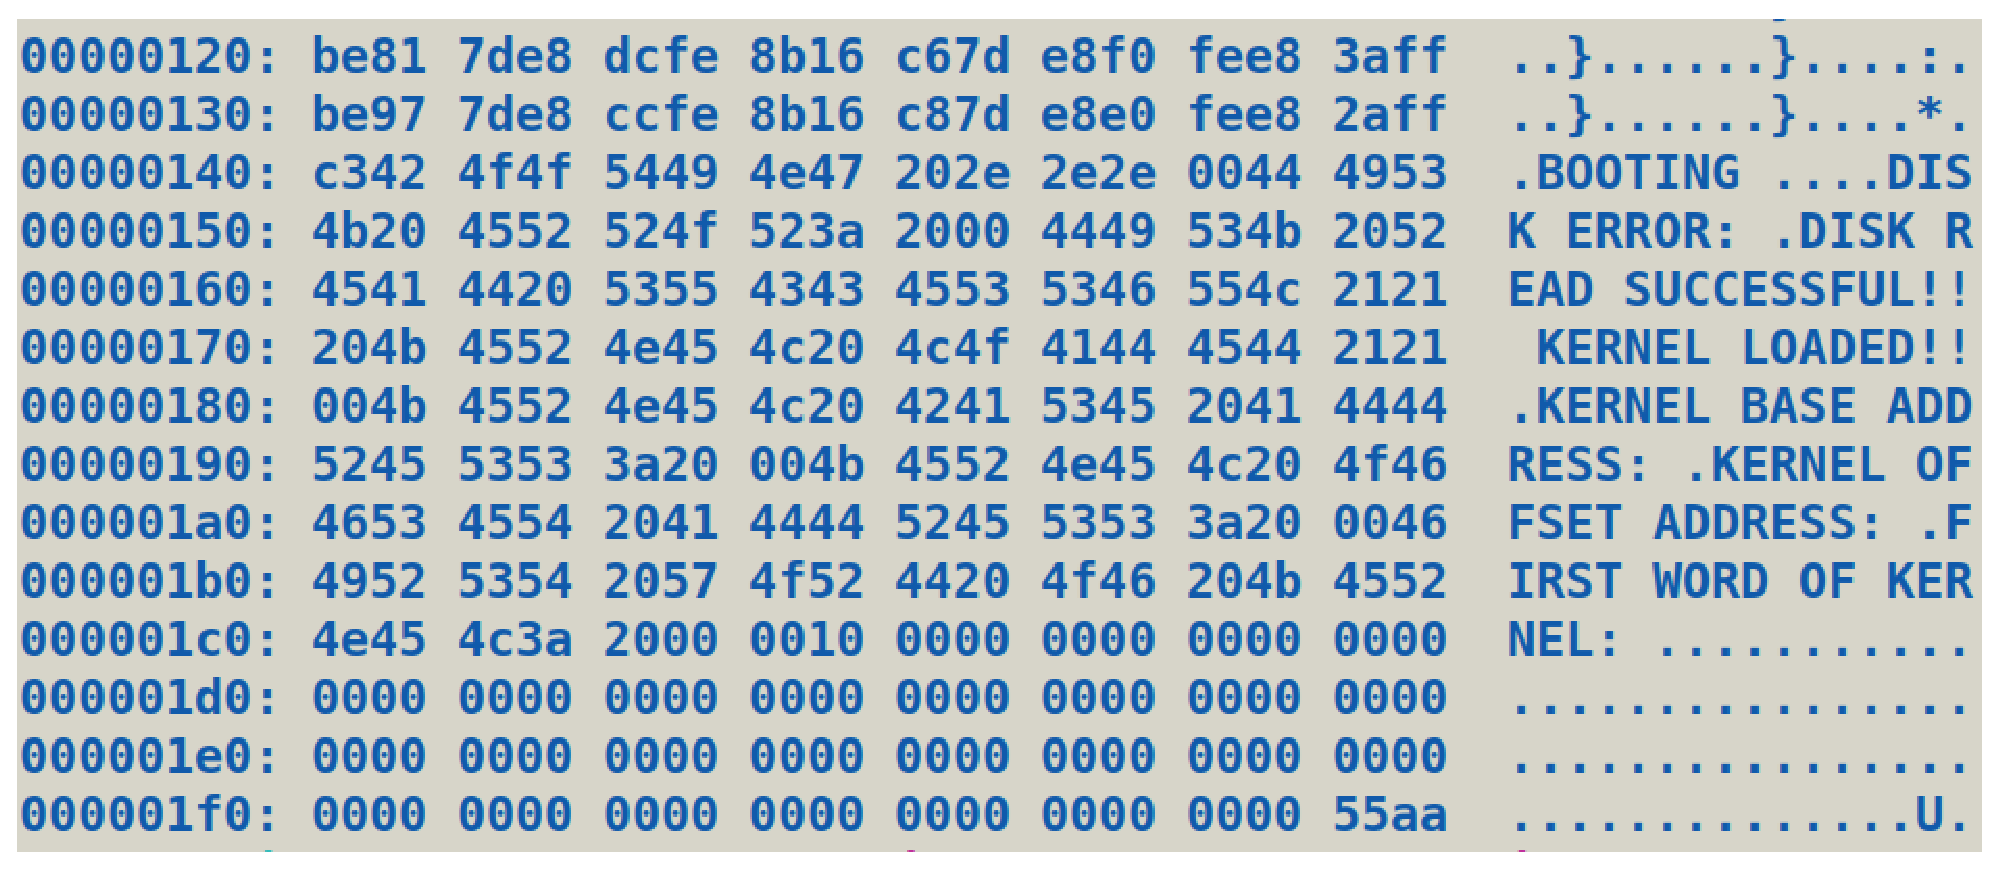
\includegraphics[scale=0.30]{figures/boothexdump.eps}
  \caption{Hexdump of the bootloader showing the placement of the magic number 0xaa55}
\label{fig:boothexdump}
\end{figure}

\subsection{boot\_util.asm}
It is important to print a few messages on the screen when the bootloader is loading the operating system. These messages especially useful in the event disk read operation has failed and the kernel has not been loaded properly. To print such messages, we make use of INT 10,0E which allows us to print characters to the screen in teletype mode. The subroutines used by the bootloader to which to print strings, newlines and hexadecimal numbers on the screen are present in \texttt{boot\_util.asm} file. These were some of the first subroutines which were developed as part of this project. These are:
\begin{enumerate}
  \item \texttt{print}
  		\begin{enumerate}[align=parleft, labelsep=2cm, leftmargin=1.06in]
  		  \item[Input]: \verb|si| = pointer to the first byte of a string
  		  \item[Output]: Nothing\footnote[1]{In context of a subroutine, the term "output" means the value that is being returned by it.}
  		  \item[Description]: Prints a null (0x00) terminated string pointed at by \verb|si|.
  		\end{enumerate}
  \item \texttt{printhex}
  		\begin{enumerate}[align=parleft, labelsep=2cm, leftmargin=1.06in]
  		  \item[Input]: \texttt{dx} = 16-bit hexadecimal number
  		  \item[Output]: Nothing
  		  \item[Description]: Prints the hexadecimal number stored in \verb|dx| in \texttt{0x\_\_\_\_} format. Uses right-shift operation \texttt{shr} and logical AND, \texttt{and}, to decompose the hexadecimal number stored in \verb|dx| into individual nibbles. A string representing the hexadecimal number is then made by adding each individual nibble to the ASCII value of either '0' or 'A' depending upon the whether it is less than 0x0a or not, respectively. The string is then printed using \texttt{print} subroutine.
  		\end{enumerate} 
  \item \texttt{printnl}
  		\begin{enumerate}[align=parleft, labelsep=2cm, leftmargin=1.06in]
  		  \item[Input]: Nothing
  		  \item[Output]: Nothing
  		  \item[Description]: Prints a newline, i.e., positions cursor at the beginning of the next line. This is achieved by printing line-feed character (0x0a) and carriage return (0x0d) using INT 10,0E. This is equivalent to \texttt{printf("\textbackslash n");} used in C programs for positioning the cursor at the beginning of the next line.
  		\end{enumerate}
\end{enumerate}

\section{Kernel Header: ../kernel/kernel.asm}
If one were to draw a memory map for CrazyOS (\autoref{fig:osmemmap}), they will find that the subroutine which is placed at the lowest memory address is the \texttt{kernel\_entry} subroutine. The operating system can be said to begin with this subroutine.
\begin{figure}[h]
  \centering
  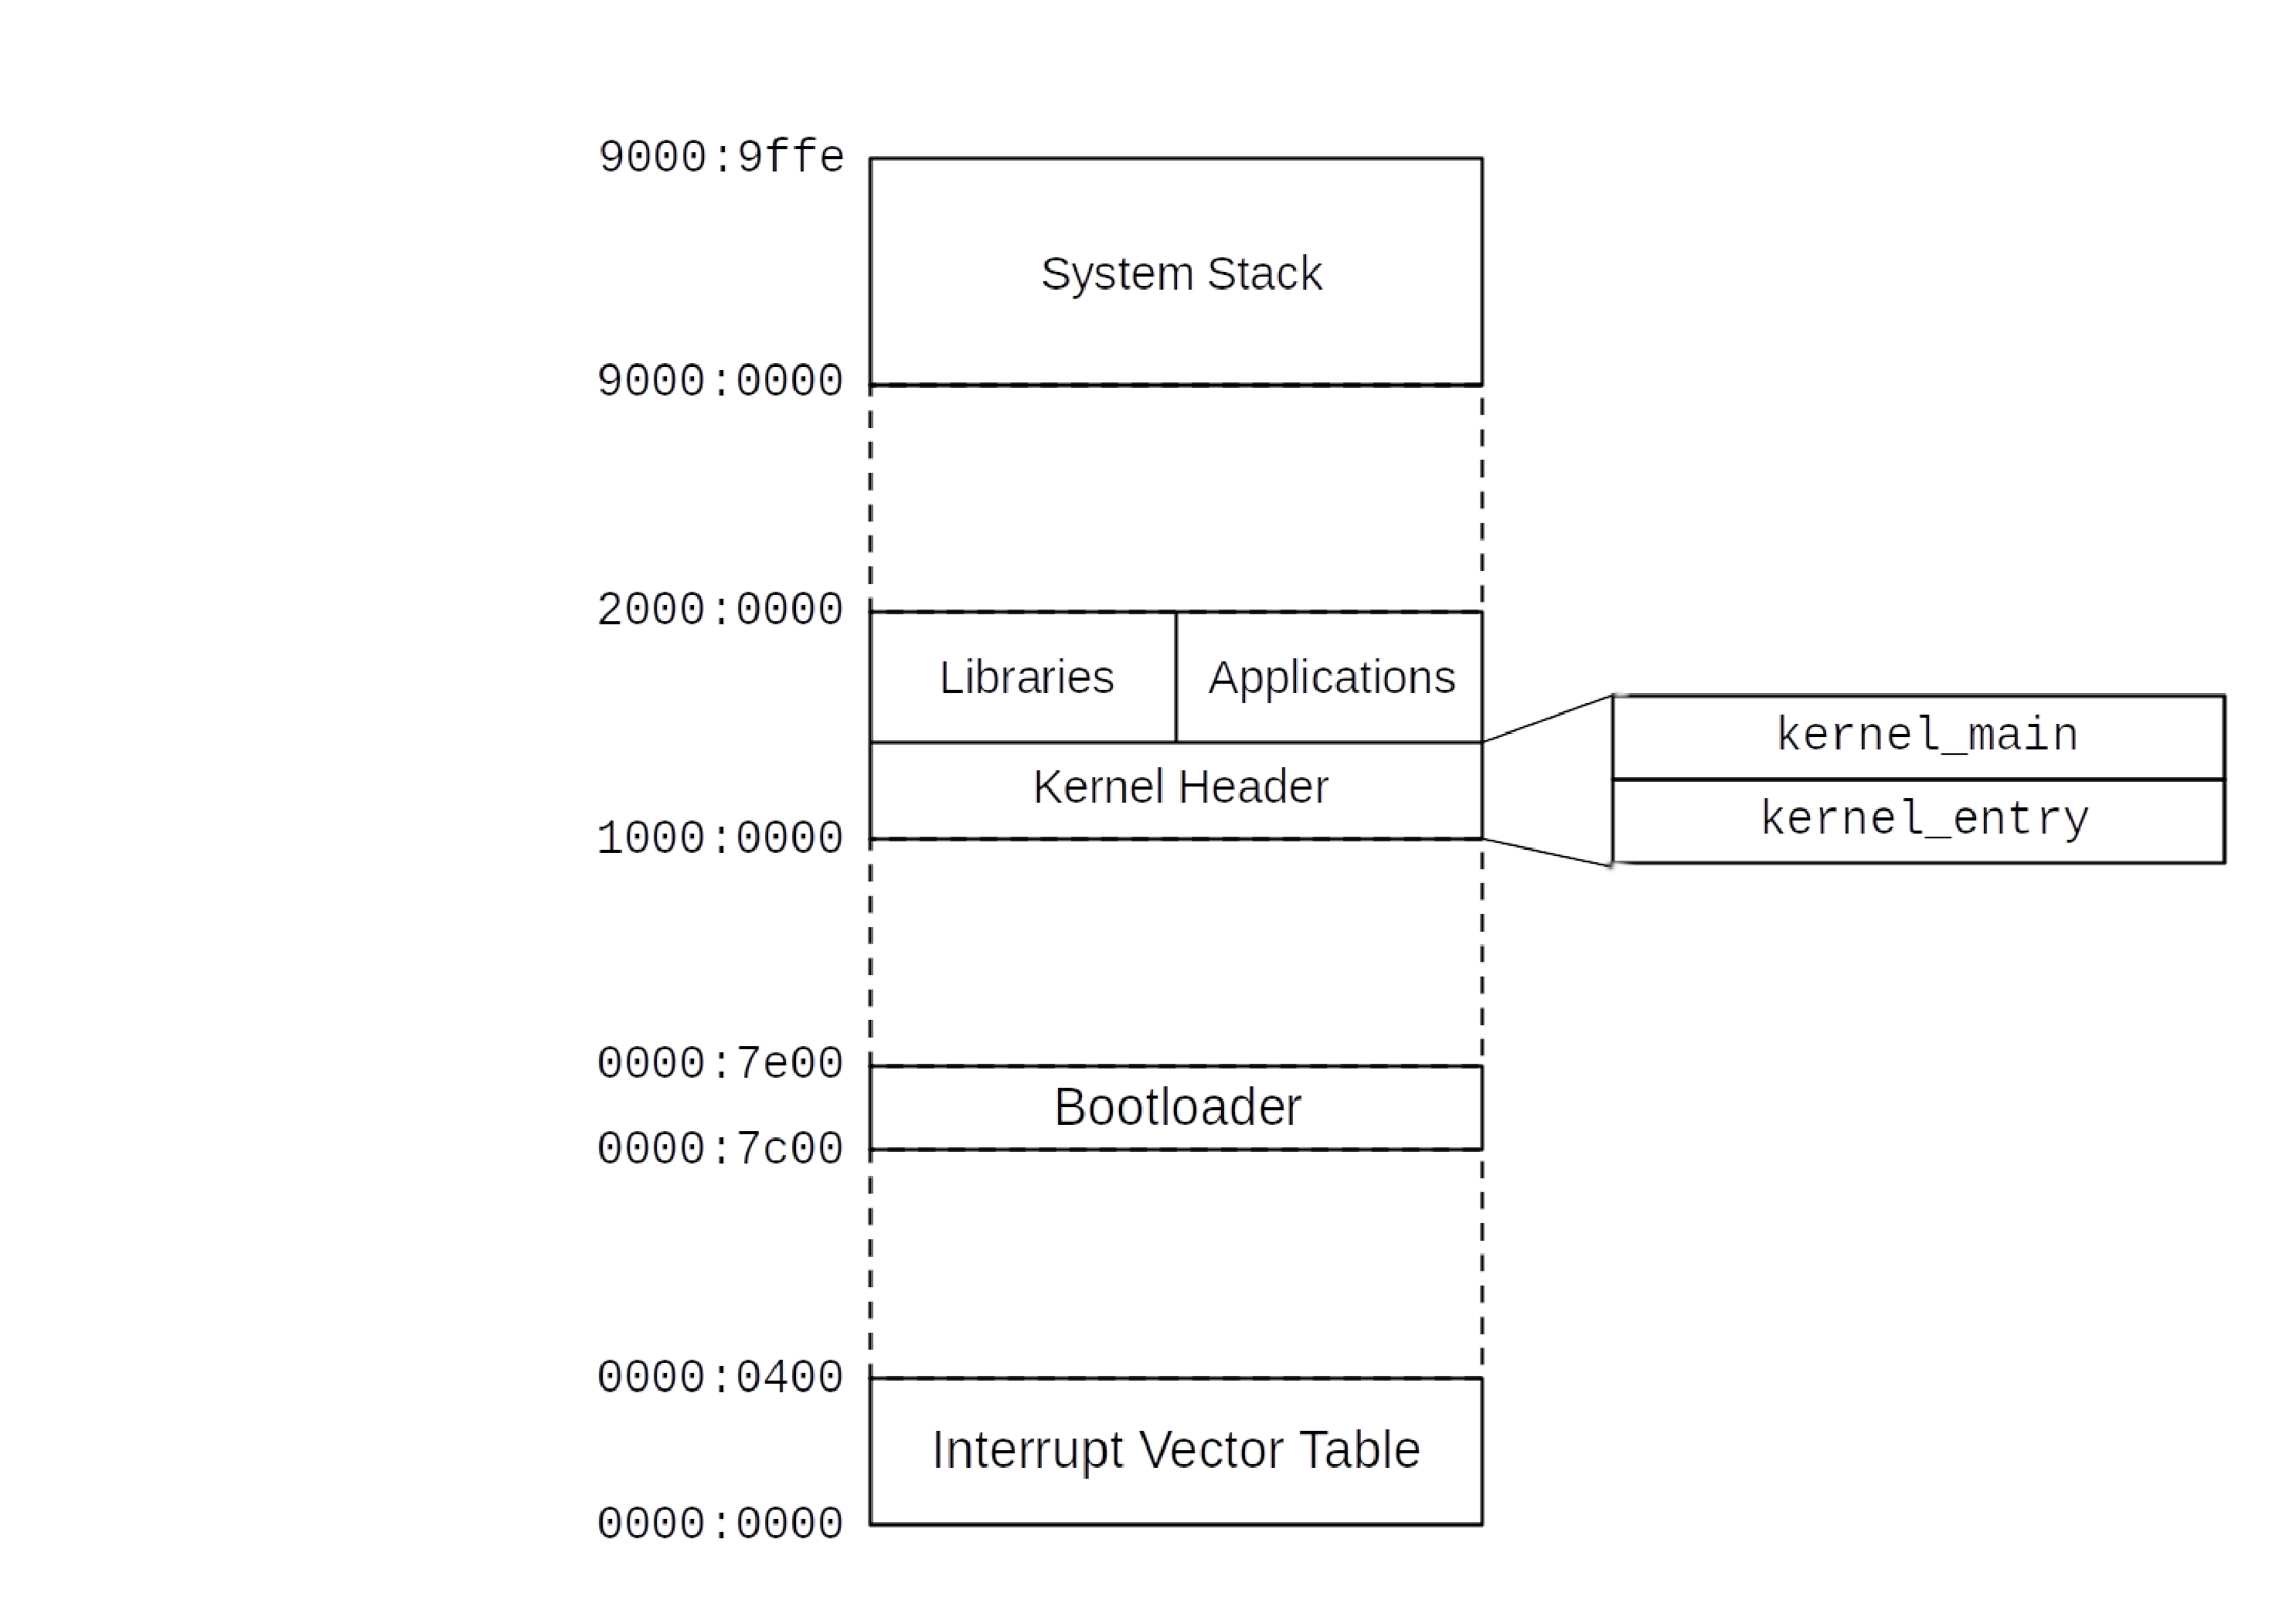
\includegraphics[scale=0.25]{figures/osmemmap.eps}
  \caption{Memory map of CrazyOS}
\label{fig:osmemmap}
\end{figure}
If \texttt{kernel.asm} forms the head of the operating system, then \texttt{kerne\_entry} subroutine would be the scalp and \texttt{kernel\_main} would be the cranium of the operating system. The bootloader performs an intersegment call to \textit{kernel\_entry} subroutine which has been loaded, along with the rest of the operating system, in block 1. \texttt{kernel\_entry} subroutine is responsible for initializing \texttt{cs}, \texttt{ds}, \texttt{es}, and \texttt{ss}.
\begin{Verbatim}
kernel_entry:
	mov ax, cs
	mov ds, ax
	mov es, ax
	mov ax, 0x9000
	mov ss, ax
	mov bp, 0x9ffe
	mov sp, bp
\end{Verbatim}
After an intersegment call has been performed by the bootloader, \texttt{cs} has been loaded with 0x1000. \verb|ds| and \verb|es| should also use the same base address as the data for the operating system has also been loaded in block 1 itself. As we cannot assign a value to segment registers directly, therefore, we store the value in \verb|cs| in \verb|ax|. Then the value stored in \verb|ax| is assigned to \verb|ds| and \verb|es|. Furthermore, we must make sure that our stack is not in the same segment as the code and data segments, otherwise problems will occur if \verb|sp| and \verb|bp| start pointing at data and instruction words. That is why the stack for the operating system is formed in block 9 which is far away from block 1. \verb|ss| is initialized with a value of 0x9000, and \verb|bp| and \verb|sp| with a value of 0x9ffe.\\
\texttt{kernel\_main} subroutine begins just after \texttt{kernel\_entry} subroutine. It is analogous to the \texttt{while(1) \{ } loop which is an infinite loop which runs a sequence of tasks again and again. \texttt{kernel\_main} clears the screen, prints a test message, date and time, and then call the \texttt{main} subroutine present in \texttt{../apps/shell.asm}.

\section{Library Functions: ../include}

\begin{figure}
\begin{forest}
  for tree={
    font=\ttfamily,
    grow'=0,
    child anchor=west,
    parent anchor=south,
    anchor=west,
    calign=first,
    edge path={
      \noexpand\path [draw, \forestoption{edge}]
      (!u.south west) +(7.5pt,0) |- node[fill,inner sep=1.25pt] {} (.child anchor)\forestoption{edge label};
    },
    before typesetting nodes={
      if n=1
        {insert before={[,phantom]}}
        {}
    },
    fit=band,
    before computing xy={l=15pt},
  }
[CrazyOS/8086/include
  [apm
    [apm\_com.asm]
    [apm.asm]
  ]
  [cmos
    [cmos\_com.asm]
    [cmos.asm]
  ]
  [disk
    [disk\_com.asm]
    [disk.asm]
  ]
  [random
    [srng.asm]
  ]
  [sound
    [sound.asm]
  ]
  [string
    [lexer.asm]
    [README.txt]
    [string.asm]
  ]
  [ttyio
    [legacyprint.asm]
    [printf.asm]
    [README.txt]
    [stdtty.asm]
    [ttyio.asm]  
  ]
]
\end{forest}
\caption{Directory tree for \texttt{CrazyOS/8086/include} (depth = 1)}
\label{fig:dirtc8include}
\end{figure}

Every operating system comes with a bunch of subroutines which are used by applications to interact with the hardware. Subroutines using which other subroutines can be built are called system calls. System calls can be issued by either calling the subroutine, or by issuing a software interrupt in the same manner a BIOS interrupt call is used to invoke the facilities provided by the BIOS. System calls and other such fundamental functions are kept in a separate directory, usually protected from user's tampering. These functions are often called library functions. In CrazyOS, these library functions are placed in \texttt{../8086/include} folder. Source tree of this directory is shown in \autoref{fig:dirtc8include}. As these functions use BIOS calls to access hardware facilities, the reader can think of BIOS interrupts as system calls. The subroutines present in the library are analogous to functions present in the standard C library such as \texttt{printf}, \texttt{scanf}, \texttt{atoi}, etc., which a programmer often uses in their application to get the job done.\\
Some of the library functions present in this directory were inspired by the standard C library functions. The rest were created as and when the need for accessing a specific piece of hardware was required. We will describe each these functions beginning with the ones which took inspiration from their standard C library counterparts. Before explaining these library functions, we will explain the organization of library files, and the \texttt{include} guard.

\subsection{Organization of Library Functions}
The first few subroutines in the library used to deal with setting up a terminal environment and handling strings. Later on, the author started dealing with device specific codes and also wrote subroutines which were executed when a command was entered in the shell. This prompted the author to organize the \texttt{../include} folder. Each subfolder in  \texttt{../include} deals with a particular component of the computer or some process. The name of the subfolder is same as the name of the device it deals with. Baring a few exceptions, subfolders present in the library contain two types of files:
\begin{enumerate}
  \item \textit{Fundamental files}: As the name speaks for itself, these files contain core subroutines which deal with devices making up the system. These subroutines might be present in different files, but are always clubbed together into a single file having the same name as that of the folder it is present in. For example, the subroutines dealing with setting up a terminal environment are present in different source files in \texttt{../include/ttyio} subdirectory, but are clubbed together into a single file named \texttt{ttyio.asm}.
  \item \textit{Command processing files}: These files contain subroutines which are executed in response to commands that has been entered in the shell. These subroutines often make use of subroutines present in fundamental files present in the same or other directories. These files also bear the same name as the folder they are present in, but have the suffix \texttt{\_com} added to them. For example, the fundamental procedures dealing with disk operations are kept in \texttt{../include/disk/disk.asm} and those procedures which are executed in response to entering of disk read/write commands in the shell are kept in \texttt{../include/disk/disk\_com.asm} file.
\end{enumerate}

\subsection{\%include Guard}
In C language, the C preprocessor processes statements which begin with \texttt{\#}. These statements are called preprocessor directives. Examples are \texttt{\# include} and \texttt{\# define} directives. The \texttt{\# include} directive is followed by the name of a file whose functions are being used in the current file. The preprocessor expands the contents of the file in place of the directive. As the size of a project grows, so does the number of source files. Including the same file more than once can cause problems during the linking stage as the linker will get confused by the multiple occurrences of the same label in different object files. To prevent such problems, The file to be included has its contents placed in between \texttt{\# ifndef}, \texttt{\# define}, and \texttt{\# endif} directives. These are called \texttt{include} guard, as they ensure that if a macro has already been declared, then there is no need to include the contents of the header file again in the final binary. For example, the first two statements of \texttt{stdio.h} file are
\begin{Verbatim}
#ifndef _STDIO_H
#define _STDIO_H		1
\end{Verbatim}
and its last statement is
\begin{Verbatim}
#endif			/* <stdio.h> included.  */
\end{Verbatim}
The contents of \texttt{stdio.h} are included between these statements. This way a programmer can include the files they think are necessary for a project and not worry about repeated inclusion of files.\\
NASM provides us with \texttt{\%ifndef}, \texttt{\%define}, and \texttt{\%endif} directives which work exactly like their C counterparts. Library subroutines often use this guard to ensure that no assembly source file is included more than once in the final binary of the project. As an example, the first few lines of \texttt{../include/ttyio/ttyio.asm} are
\begin{Verbatim}
bits 16
align 16
%ifndef TTYIO
%define TTYIO
%include "include/ttyio/legacyprint.asm"
%include "include/ttyio/printf.asm"
%include "include/ttyio/stdtty.asm"
\end{Verbatim}

and its closing line is
\begin{Verbatim}
%endif
\end{Verbatim}

\subsection{Standard I/O subroutines: ../include/ttyio}
A programmer just needs to include \texttt{ttyio.asm} file in his source file to get access to all the functions which are available for printing on the screen and for taking input from the keyboard. The file \texttt{ttyio.asm} contains a single subroutine, \texttt{fstringdata}, with the rest coming from inclusion of \texttt{legacyprint.asm}, \texttt{printf.asm}, and \texttt{stdtty.asm}. \texttt{fstringdata} can be described as follows:
\begin{enumerate}
  \item[]\texttt{fstringdata}
\begin{enumerate}[align=parleft, labelsep=2cm, leftmargin=1.5in]
  		  \item[Input]: \texttt{si} = pointer to a null terminated string, \newline\texttt{ax} = data to be entered,\newline\texttt{cx} = position at which data is to be entered
  		  \item[Output]: Nothing 
  		  \item[Description]: Used to enter data next to a null-terminated formatted string.
  		\end{enumerate}
\end{enumerate}
\texttt{legacyprint.asm} was the first library file which was written for this project. Two functions, namely, \verb|print|, and \texttt{printnl}, have been directly copied from \texttt{../boot/boot\_util.asm}. \texttt{printhex} subroutine present in this file bears the same name as its counterpart which was used in the bootloader to print hexadecimal numbers. However, this version of \texttt{printhex} uses right rotation instruction, \verb|ror|, to decompose the 16-bit hexadecimal number stored in \textbf{\texttt{ax}} into nibbles. Other functions which have been included in this file are: 
\begin{enumerate}
  \item \texttt{print8bitpackedBCD}
  		\begin{enumerate}[align=parleft, labelsep=2cm, leftmargin=1.06in]
  		  \item[Input]: \texttt{ah} = 0x00,\newline\texttt{al} = 8-bit packed BCD
  		  \item[Output]: Nothing
  		  \item[Description]: Prints an 8-bit packed BCD stored in \texttt{al}.
  		\end{enumerate}
  \item \texttt{printdec}
  		\begin{enumerate}[align=parleft, labelsep=2cm, leftmargin=1.06in]
  		  \item[Input]: \texttt{ax} = 16-bit number (0 - 65535)
  		  \item[Output]: Nothing
  		  \item[Description]: Prints a 16-bit number stored in \texttt{ax} in decimal format. A blank space is printed if the number is equal to 0.
  		\end{enumerate}
\end{enumerate}
\texttt{stdtty.asm} defines several subroutines which enable the user to print characters on the screen as well as take input from the keyboard. The functions defined in this source file are:
\begin{enumerate}
  \item \texttt{clear}
  		\begin{enumerate}[align=parleft, labelsep=2cm, leftmargin=1.06in]
  		  \item[Input]: Nothing
  		  \item[Output]: Nothing
  		  \item[Description]: Similar to the working of \texttt{clrscr} subroutine in \texttt{../boot/boot.asm}, this subroutine clears the screen, sets page-number to 0, resets background and foreground colour to their default values, and positions the cursor at row 0 and column 0. Executed when \texttt{clear} command is entered in the shell.
  		\end{enumerate}
  \item \texttt{findcursorposition}
  		\begin{enumerate}[align=parleft, labelsep=2cm, leftmargin=1.06in]
  		  \item[Input]: Nothing
  		  \item[Output]: \texttt{dh} = row at which the cursor is positioned (0 - 24),\newline\texttt{dl} = column at which the cursor is positioned (0 - 79)
  		  \item[Description]: Used to find the position of the cursor. 
  		\end{enumerate}
  \item \texttt{scrollup}
  		\begin{enumerate}[align=parleft, labelsep=2cm, leftmargin=1.06in]
  		  \item[Input]: Nothing
  		  \item[Output]: Nothing
  		  \item[Description]: Scrolls the screen up by a single line only
  		\end{enumerate}
  \item \texttt{conditional\_scrollup}
  		\begin{enumerate}[align=parleft, labelsep=2cm, leftmargin=1.06in]
  		  \item[Input]: Nothing
  		  \item[Output]: Nothing
  		  \item[Description]: Finds the position of the cursor and scrolls the screen up by a single line if the cursor is found to be positioned at the 24th row.
  		\end{enumerate}
  \item \texttt{putchar}
  		\begin{enumerate}[align=parleft, labelsep=2cm, leftmargin=1.06in]
  		  \item[Input]: \texttt{al} = code of the character to be printed from code page 437
  		  \item[Output]: Nothing
  		  \item[Description]: Prints a single character onto the screen. Calls \texttt{conditional\_scrollup} and \texttt{printnl} to scroll the screen up by one line in case the cursor is at 24th row.
  		\end{enumerate}
  \item \texttt{getchar}
  		\begin{enumerate}[align=parleft, labelsep=2cm, leftmargin=1.06in]
  		  \item[Input]: Nothing
  		  \item[Output]: \texttt{ah} = keyscan code of the key combination that has been pressed, \texttt{al} = code of the character corresponding to the key combination that has been pressed. 
  		  \item[Description]: Reads a key from the keyboard and returns the corresponding key scan codes and character code in \texttt{ah} and \texttt{al}, respectively.
  		\end{enumerate}
  \item \texttt{getline}
  		\begin{enumerate}[align=parleft, labelsep=2cm, leftmargin=1.06in]
  		  \item[Input]: Nothing
  		  \item[Output]: \texttt{si} = pointer to the 80-byte wide buffer, \texttt{GETLINE\_BUFFER}
  		  \item[Description]: Allows the user to input a single line, having a maximum length of 80 characters, through the keyboard. Printable ASCII characters are printed on the screen. Rest of the characters perform control sequence such as deleting a character, positioning the cursor, etc. Not all cursor control sequences are supported. \texttt{si} is returned as a pointer to the \texttt{GETLINE\_BUFFER}.
  		\end{enumerate}
  \item \texttt{flush}
  		\begin{enumerate}[align=parleft, labelsep=2cm, leftmargin=1.06in]
  		  \item[Input]: Nothing
  		  \item[Output]: Nothing
  		  \item[Description]: Flushes the \texttt{GETLINE\_BUFFER} by setting all 80 bytes it is made up of equal to 0x00.
  		\end{enumerate}
\end{enumerate}
Finally, we come to \texttt{printf.asm} which has the source code for a bare-minimum implementation of \texttt{printf} found in C.
\begin{enumerate}
  \item[]\texttt{printf}
  		\begin{enumerate}[align=parleft, labelsep=2cm, leftmargin=1.06in]
  		  \item[Input]: \texttt{si} = pointer to a null-terminated string followed by optional data to be printed.
  		  \item[Output]: Nothing
  		  \item[Description]: A bare-minimum implementation of \texttt{printf}. Data which is to be printed should have word size and should be entered after terminating null word of the string using \texttt{fstringdata} subroutine. Supported format specifiers are:
  		  \begin{enumerate}[align=parleft, labelsep=2cm]
  		    \item[]\verb|%c|: Single character
  		    \item[]\verb|%d|: 16-bit number in decimal format
  		    \item[]\verb|%x|: 16-bit number in hexadecimal format
  		  \end{enumerate}
Supported escape sequences are:
  		  \begin{enumerate}[align=parleft, labelsep=2cm]
  		    \item[]\verb|\n|: Newline
  		    \item[]\verb|\t|: Tab
  		  \end{enumerate}
  		\end{enumerate}
\end{enumerate}

\subsection{String Handling: ../include/string}
String handling is an important part of any language. The programmer who is writing applications for CrazyOS has to include \texttt{../include/string/string.asm} in his application program to allow him to use various subroutines to handle strings. These subroutines have been inspired from their counterparts found in \texttt{string.h} in C. These subroutines have been described below:
\begin{enumerate}
  \item \texttt{strlen}
  		\begin{enumerate}[align=parleft, labelsep=2cm, leftmargin=1.06in]
  		  \item[Input]: \texttt{si} = pointer to a null-terminated string
  		  \item[Output]: \texttt{ax} = length of the string pointed at by \texttt{si}
  		  \item[Description]: Used to compute the length of the string.
  		\end{enumerate}
  \item \texttt{strcmp}
  		\begin{enumerate}[align=parleft, labelsep=2cm, leftmargin=1.06in]
  		  \item[Input]: \texttt{si} = pointer to the first null-terminated string,\newline\texttt{di} = pointer to the second null-terminated string
  		  \item[Output]: \texttt{ax} = 0x00 if the the strings are equal, or\newline\texttt{ax} = 0x01 if the strings are not equal
  		  \item[Description]: Compares two strings which are being pointed at by \texttt{si} and \texttt{di}. It first compares their length using \texttt{strlen} subroutine. If the lengths are found to be equal, it then compares them character by character. If both the strings are found to be equal to each other, then \texttt{ax} is returned with 0x00, else \texttt{ax} is set to 0x01
  		\end{enumerate}
  \item \texttt{strcpy}
  		\begin{enumerate}[align=parleft, labelsep=2cm, leftmargin=1.06in]
  		  \item[Input]: \texttt{si} = pointer to the null-terminated source string,\newline\texttt{di} = pointer to the destination string
  		  \item[Output]: Nothing
  		  \item[Description]: Copies the source string pointed at by \texttt{si} to the destination string pointed at by \texttt{di}. \texttt{rep movsb} instruction is used to perform this copying operation.
  		\end{enumerate}
  \item \texttt{atoi}
  		\begin{enumerate}[align=parleft, labelsep=2cm, leftmargin=1.06in]
  		  \item[Input]: \texttt{si} = pointer to the string representation of a 16-bit positive number.
  		  \item[Output]: \texttt{ax} = number which was stored in the string pointed at by \texttt{si}
  		  \item[Description]: Converts the string representation of a number to a 16-bit number, stores it in \texttt{ax}, and returns to the caller.
  		\end{enumerate}
  \item \texttt{atoh}
  		\begin{enumerate}[align=parleft, labelsep=2cm, leftmargin=1.06in]
  		  \item[Input]: \texttt{si} = pointer to the string representation of a hexadecimal number
  		  \item[Output]: \texttt{ax} = hexadecimal number which was stored in string format
  		  \item[Description]: Converts the string representation of a hexadecimal number, stores it in \texttt{ax}, and returns to the caller. Although the prefix "0x" is used when printing hexadecimal numbers, it should be made sure that the string being passed to atoh does not have this prefix.
  		\end{enumerate}
\end{enumerate}

\texttt{..include/string} directory has another assembly source file besides \texttt{string.asm}. It is \texttt{lexer.asm} which is responsible for breaking a string of characters into separate "words" using some separator. The function used for performing this primitive lexical-analysis is \texttt{cmd\_lexer}. Its description is given below:
\begin{enumerate}
  \item[] \texttt{cmd\_lexer}
  		\begin{enumerate}[align=parleft, labelsep=2cm, leftmargin=1.06in]
  		  \item[Input]: \texttt{al} = ASCII code of the character to be used as a separator,\newline\texttt{si} = pointer to the 80-byte wide string
  		  \item[Output]: Nothing
  		  \item[Description]: \textit{Tokenizes} the string that is being pointed at by \texttt{si} using the character stored in \texttt{al} as a separator. It generates its own personal copy of the string which is stored in local label \texttt{.COPY}. This subroutine is capable of generating a maximum of 5 tokens: one command token and four argument tokens. Command token is stored in global label \texttt{com} and argument tokens are stored in \texttt{arg1}, \texttt{arg2}, \texttt{arg3}, and \texttt{4} which are also global labels.
  		\end{enumerate}
\end{enumerate} 
\subsection{CMOS and RTC: ..include/cmos}
Real time clock, or RTC for short, is responsible for keeping track of date and time even when the computer has been turned off. This is achieved by independently powering the RTC using a CR2032 coin cell. As the power consumption of RTC is very small, one coin cell lasts for many years. The RTC chip also has very low power static CMOS memory. Although the term CMOS specifically refers to a type of semiconductor technology, when used in context with personal computers, the term refers to the static memory on the RTC chip. This memory has several registers which store setup information for the BIOS even when the computer is turned off. The first 14 CMOS registers store the time and date and control the operation of the RTC. CMOS registers can be accessed using \verb|in| and \verb|out| instructions. CMOS's input is mapped to port 0x70 and its output is mapped to 0x71. Before writing anything to these ports the interrupts must be disabled using \verb|cli|. They can later be enabled using \verb|sti|. To read the value of a CMOS register, we store the register number in \verb|al| and then execute the following instructions:
\begin{Verbatim}
        cli
        out 0x70, al
        nop
        in al, 0x71
        sti
\end{Verbatim}
The value of the register is returned in \verb|al|. To write a value to a CMOS register, we first select the register by passing its number to port 0x70. Then write the value to be written at port 0x71. The code for the same is shown below:
\begin{Verbatim}
        cli
        out 0x70, al
        nop
        mov al, bl 
        out 0x71, al
        sti
\end{Verbatim}
Simple subroutines to read and write CMOS registers are kept in \texttt{cmos.asm} file. These subroutines are:
\begin{enumerate}
  \item \texttt{read\_cmos}
  		\begin{enumerate}[align=parleft, labelsep=2cm, leftmargin=1.06in]
  		  \item[Input]: \texttt{al} = index of the register to be accessed
  		  \item[Output]: \texttt{al} = value of the register that was accessed
  		  \item[Description]: Used to read the value of a register. Interrupts are disabled before executing port I/O instructions and are enabled before returning to the caller. A \texttt{nop} instruction is executed between two consecutive port operations. This gives the system enough time to perform port operation correctly.
  		\end{enumerate}
  \item \texttt{write\_cmos}
  		\begin{enumerate}[align=parleft, labelsep=2cm, leftmargin=1.06in]
  		  \item[Input]: \texttt{al} = index of the register to be accessed,\newline\texttt{bl} = value to be written to the register
  		  \item[Output]: Nothing
  		  \item[Description]: Writes a value passed in \texttt{bl} to the CMOS register with index equal to the value stored in \texttt{al}.
  		\end{enumerate}
\end{enumerate}
\texttt{cmos\_com.asm} contains subroutines which are executed when \texttt{date} or \texttt{time} commands are entered in the shell. These subroutines are:
\begin{enumerate}
  \item \texttt{time}
  		\begin{enumerate}[align=parleft, labelsep=2cm, leftmargin=1.06in]
  		  \item[Input]: Nothing
  		  \item[Output]: Nothing
  		  \item[Description]: Global variables \texttt{HRS}, \texttt{MIN}, and \texttt{SEC} are updated with the value of hour, minutes, seconds at the time of execution of the function, respectively.
  		\end{enumerate}
  \item \texttt{showtime}
  		\begin{enumerate}[align=parleft, labelsep=2cm, leftmargin=1.06in]
  		  \item[Input]: Nothing
  		  \item[Output]: Nothing
  		  \item[Description]: Prints time in \texttt{HH:MM:SS} format. Hour is printed in 24-hour format. Executed when \texttt{time} command is entered in the shell.
  		\end{enumerate}
  \item \texttt{date}
  		\begin{enumerate}[align=parleft, labelsep=2cm, leftmargin=1.06in]
  		  \item[Input]: Nothing
  		  \item[Output]: Nothing
  		  \item[Description]: Global variables \texttt{WEEKDAY}, \texttt{DAY\_OF\_THE\_MONTH}, \texttt{MONTH}, and \texttt{YEAR} are updated with the value of current index of weekday (Sunday = 1, Monday = 2, etc.), day of the month, month number, and last two digits of the year at the time of execution of the function, respectively.
  		\end{enumerate}
  \item \texttt{showdate}
  		\begin{enumerate}[align=parleft, labelsep=2cm, leftmargin=1.06in]
  		  \item[Input]: Nothing
  		  \item[Output]: Nothing
  		  \item[Description]: Displays current date in \texttt{Weekday, DD-MM-YY} format. Executed when \texttt{date} command is entered in the shell.
  		\end{enumerate}
\end{enumerate}

\subsection{Random Number Generator: ../include/random}
Random number generators often find application in games, cryptography, and computer simulation. The author has written a simple pseudo-random number generator, \texttt{srng}. It is described as follow:
\begin{enumerate}
  \item[]\texttt{srng}
  		\begin{enumerate}[align=parleft, labelsep=2cm, leftmargin=1.06in]
  		  \item[Input]: Nothing 
  		  \item[Output]: \texttt{ax} = pseudo-random number
  		  \item[Description]: Produces a pseudo-random number by taking the value of seconds elapsed as a seed value. This value is obtained from register 0x00 of the CMOS. This seed value is multiplied with 8999d, which is a prime number. 9923d, which is another prime number, is added to the product's low byte to produce a pseudo-random number which is returned in \texttt{ax}. 
  		\end{enumerate}
\end{enumerate}

\subsection{Sound Generator: ../include/sound}
Before discussing the process of sound generation in an IBM PC, we must briefly discuss the 8254 programmable interval timer (PIT) chip. This chip was primarily designed to solve timing control problems in microcomputers. Its block diagram is shown in \autoref{fig:8254}.

\begin{figure}[h]
  \centering
  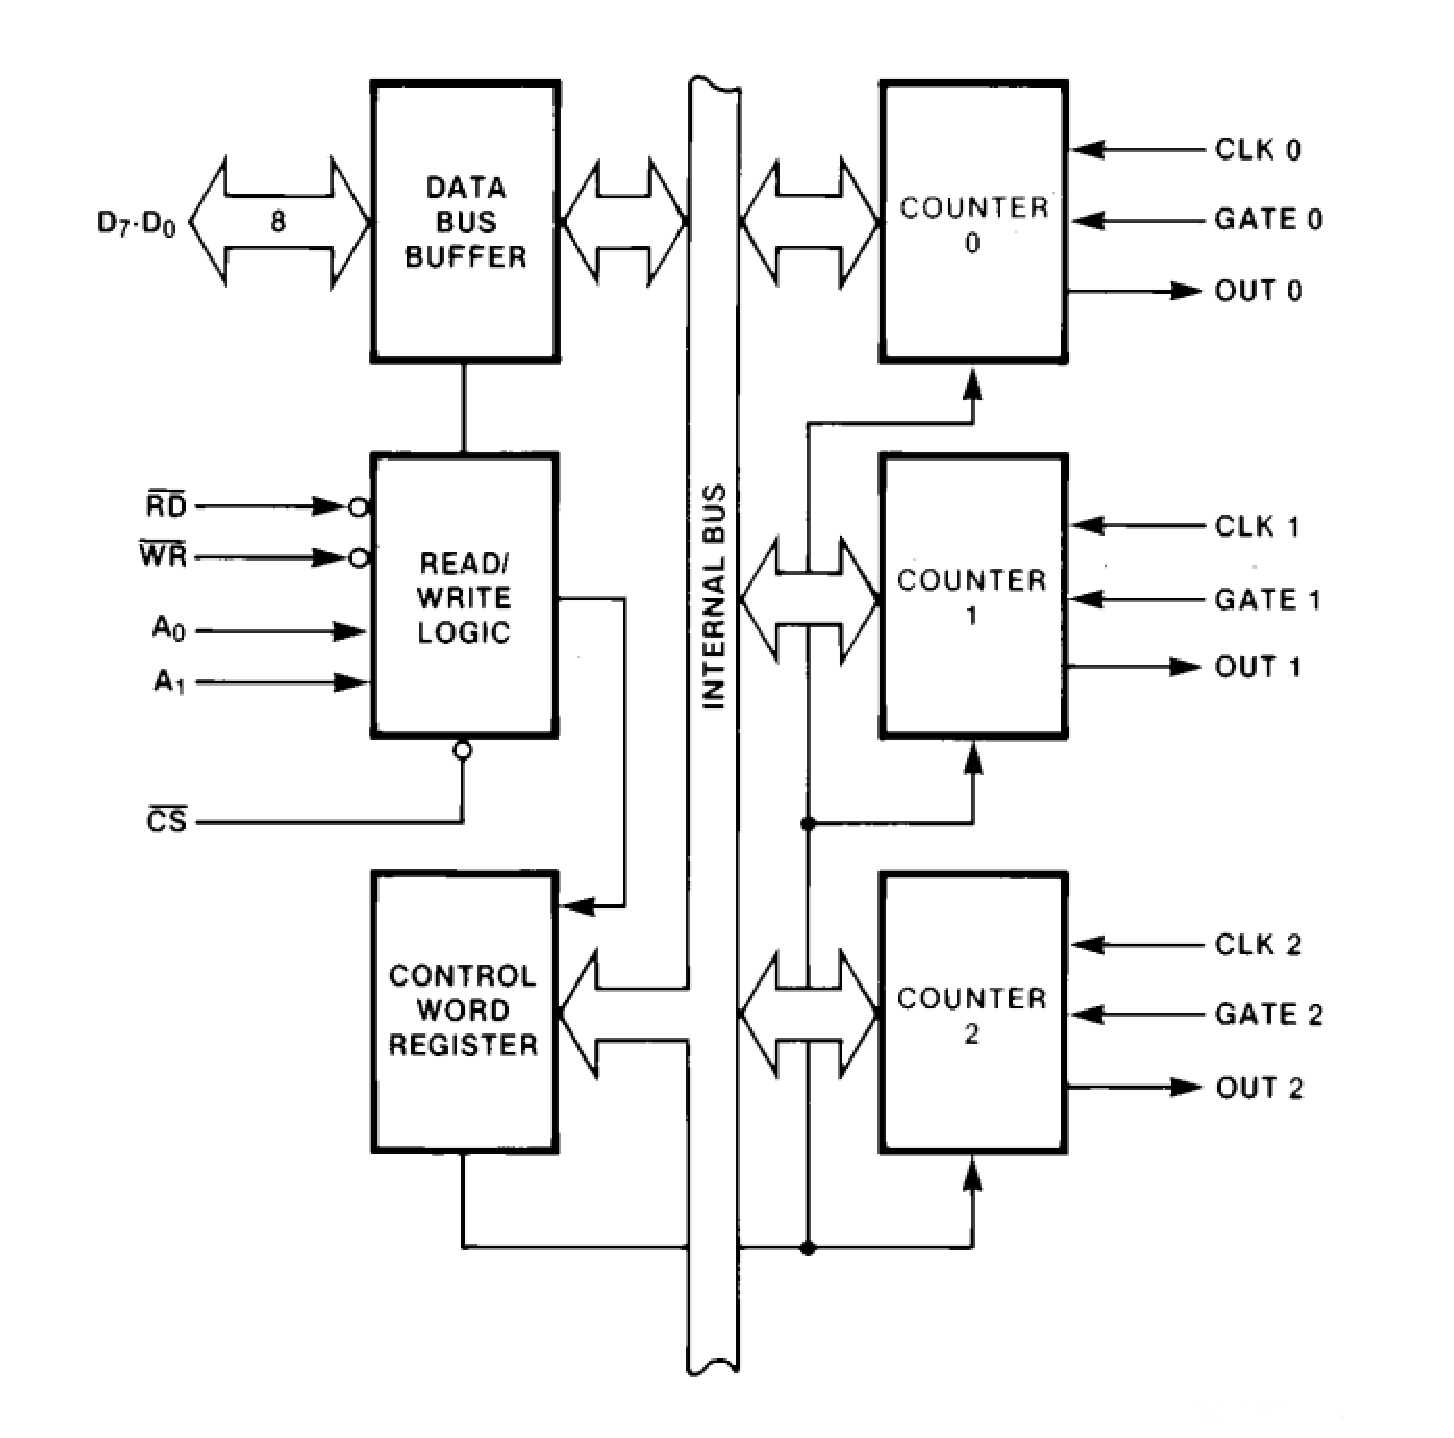
\includegraphics[scale=0.30]{figures/8254.eps}
  \caption{Block diagram of the 8254 PIT chip \cite{intel1993PIT}}
\label{fig:8254}
\end{figure}

It consists of 3 counters/timers, each capable of working independently of each other. Numbering of timers start from 0. Therefore, we have timer 0, timer 1, and timer 2. The mode in which each timer operates is decided by the value which has been passed to the control word register. The format of the word which is passed on to the control word register is shown in \autoref{fig:8254cwr}. On an IBM PC, control word register is mapped to port 0x43. Once the control word has been transmitted, the counter of each timer needs to be initialized with some value. Count down starts from this value. The counters of timers are also mapped to I/O ports starting from port 0x40. So, timer 0's counter is mapped to port 0x40, timer 1's counter is mapped to port 0x41, and timer 2's counter is mapped to port 0x42. Each timer/channel two input pins, namely \texttt{CLK} and \texttt{GATE}. The former receives clock signal from an oscillator running at approximately 1.19 MHz. The later is used to enable an output signal from the output pin, \texttt{OUT} \cite{intel1993PIT}.

\begin{figure}[h]
  \centering
  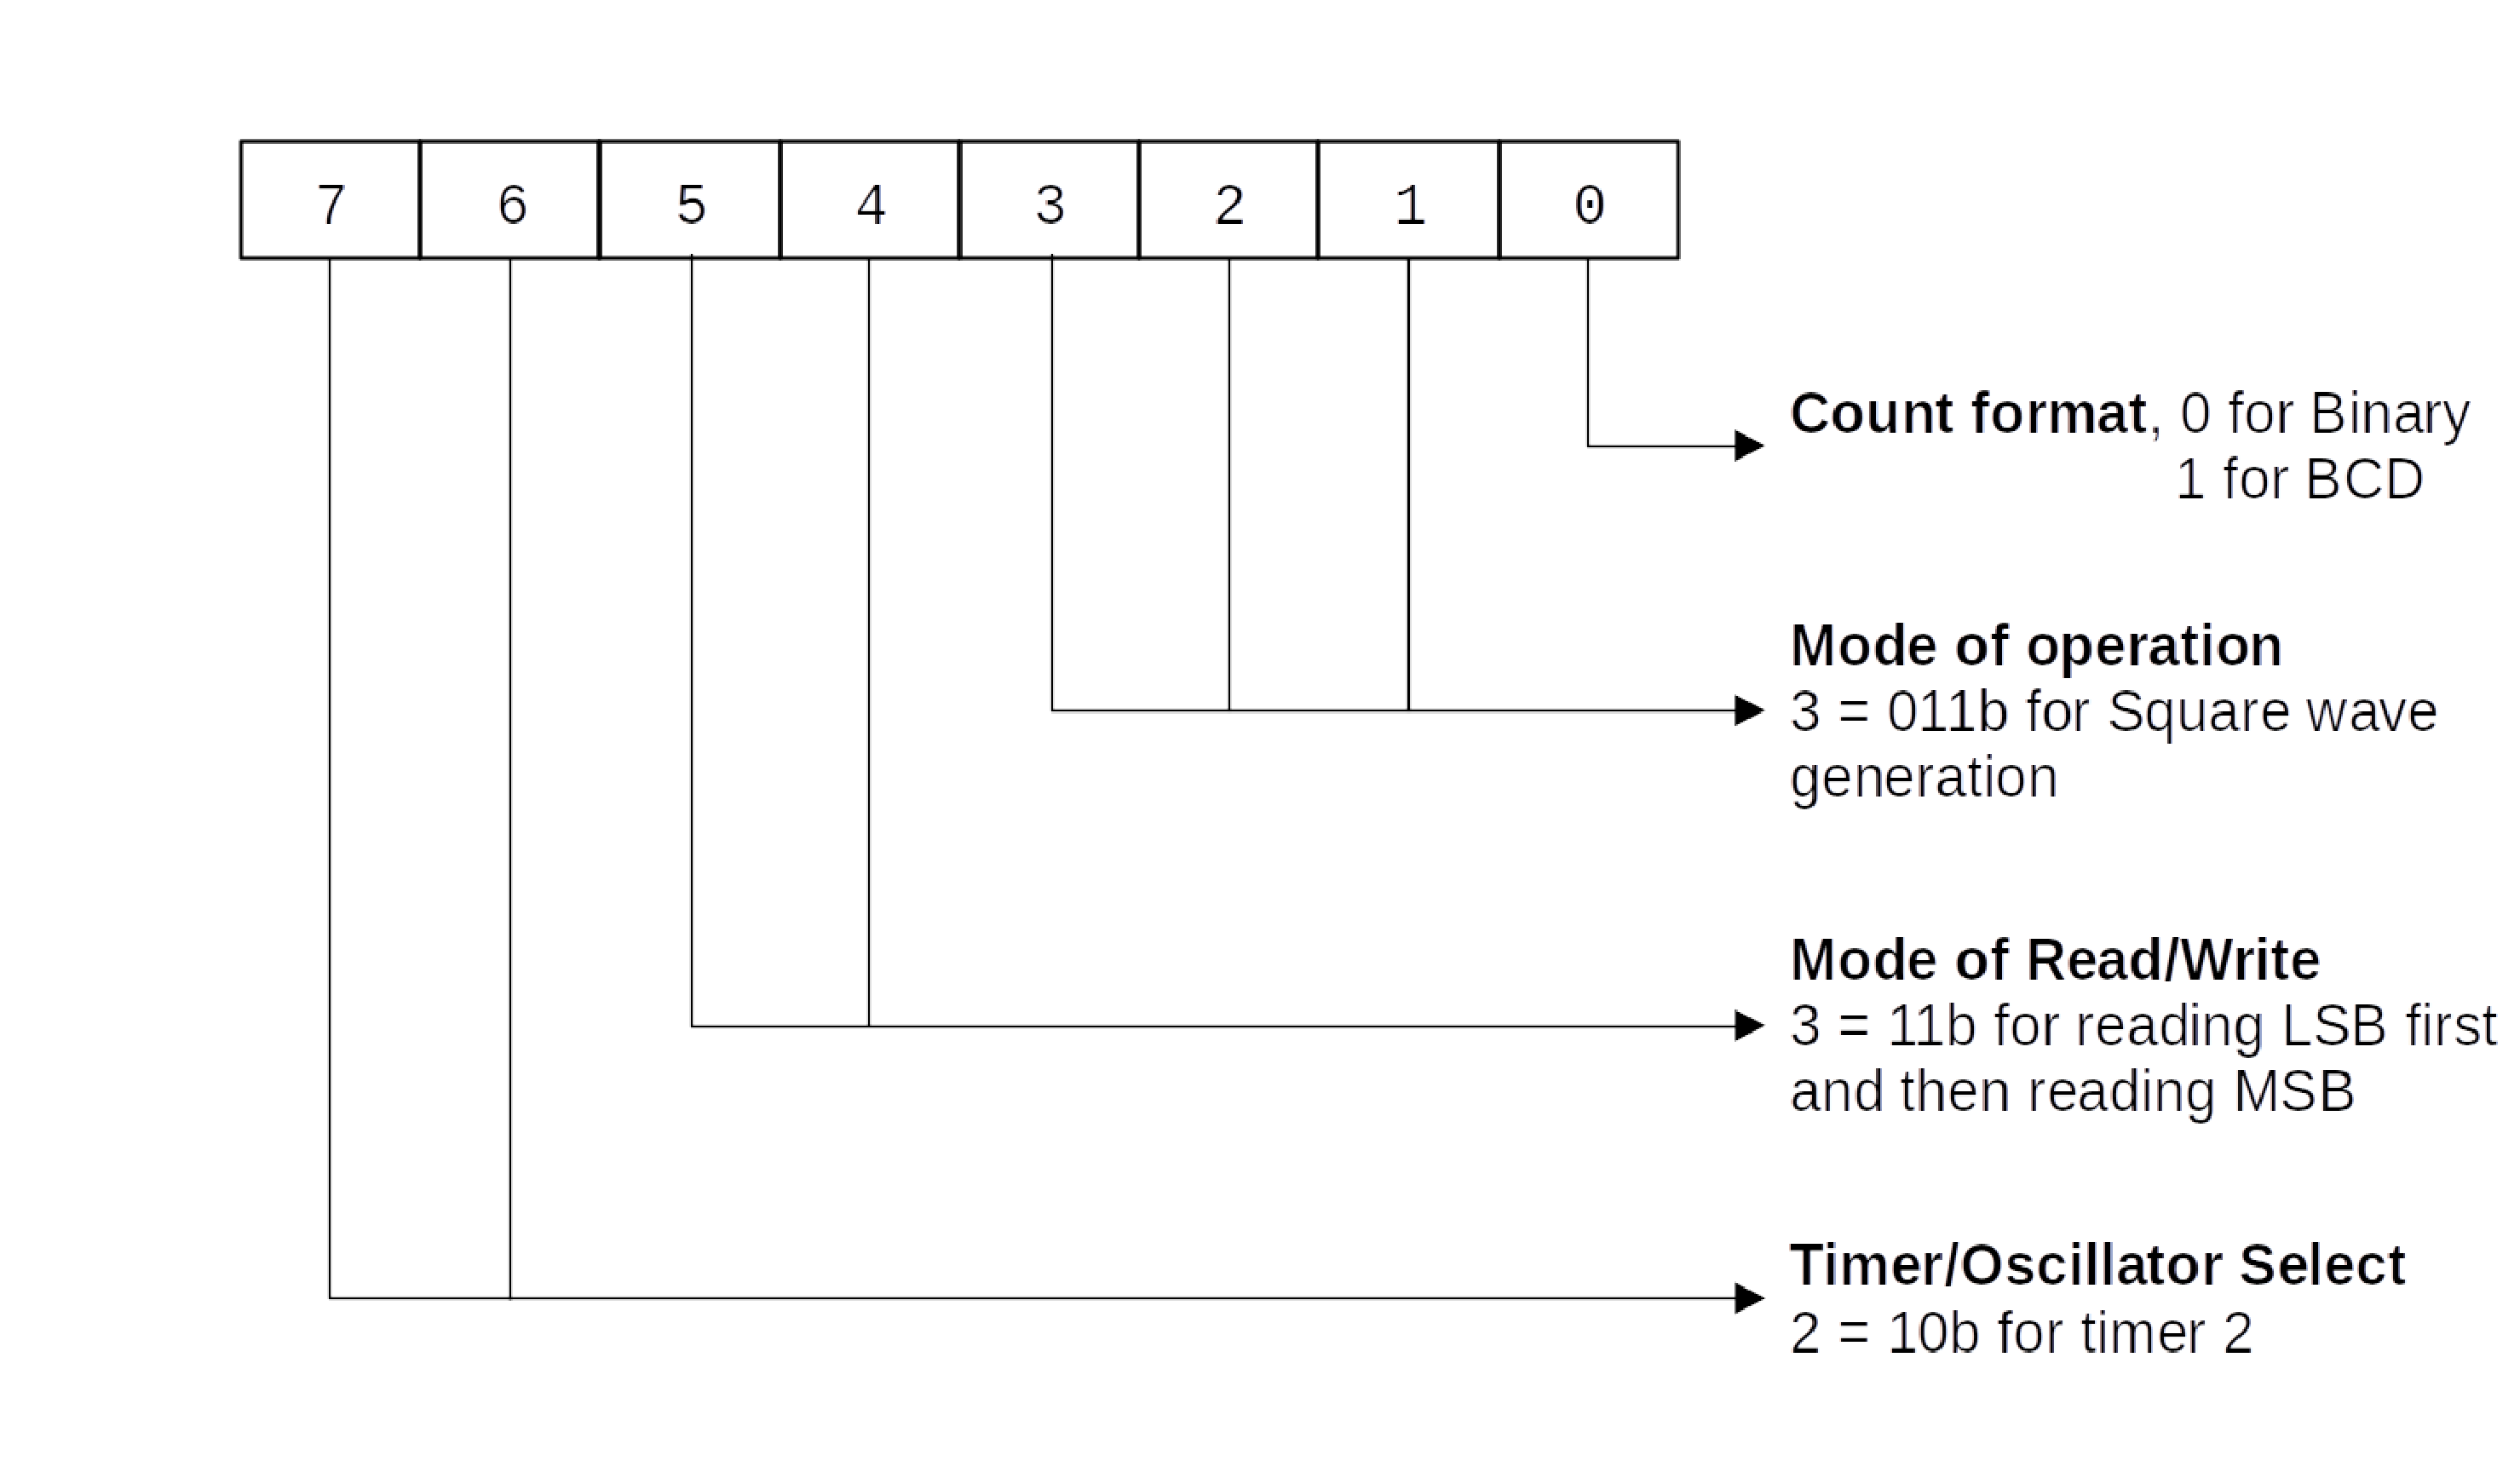
\includegraphics[scale=0.25]{figures/8254cwr.eps}
  \caption{Control word format for the PIT chip}
\label{fig:8254cwr}
\end{figure}

We are interested in operating the piezoelectric speaker which is soldered onto the motherboard of PCs. This piezoelectric speaker is driven by the signal generated by timer 2, and is connected to its \texttt{OUT} line using an AND gate as shown in \autoref{fig:speakermap}. The second pin of this AND gate is mapped to bit 1 of port 0x61. \texttt{GATE 2} pin is mapped to bit 0 of port 0x61.

\begin{figure}[h]
  \centering
  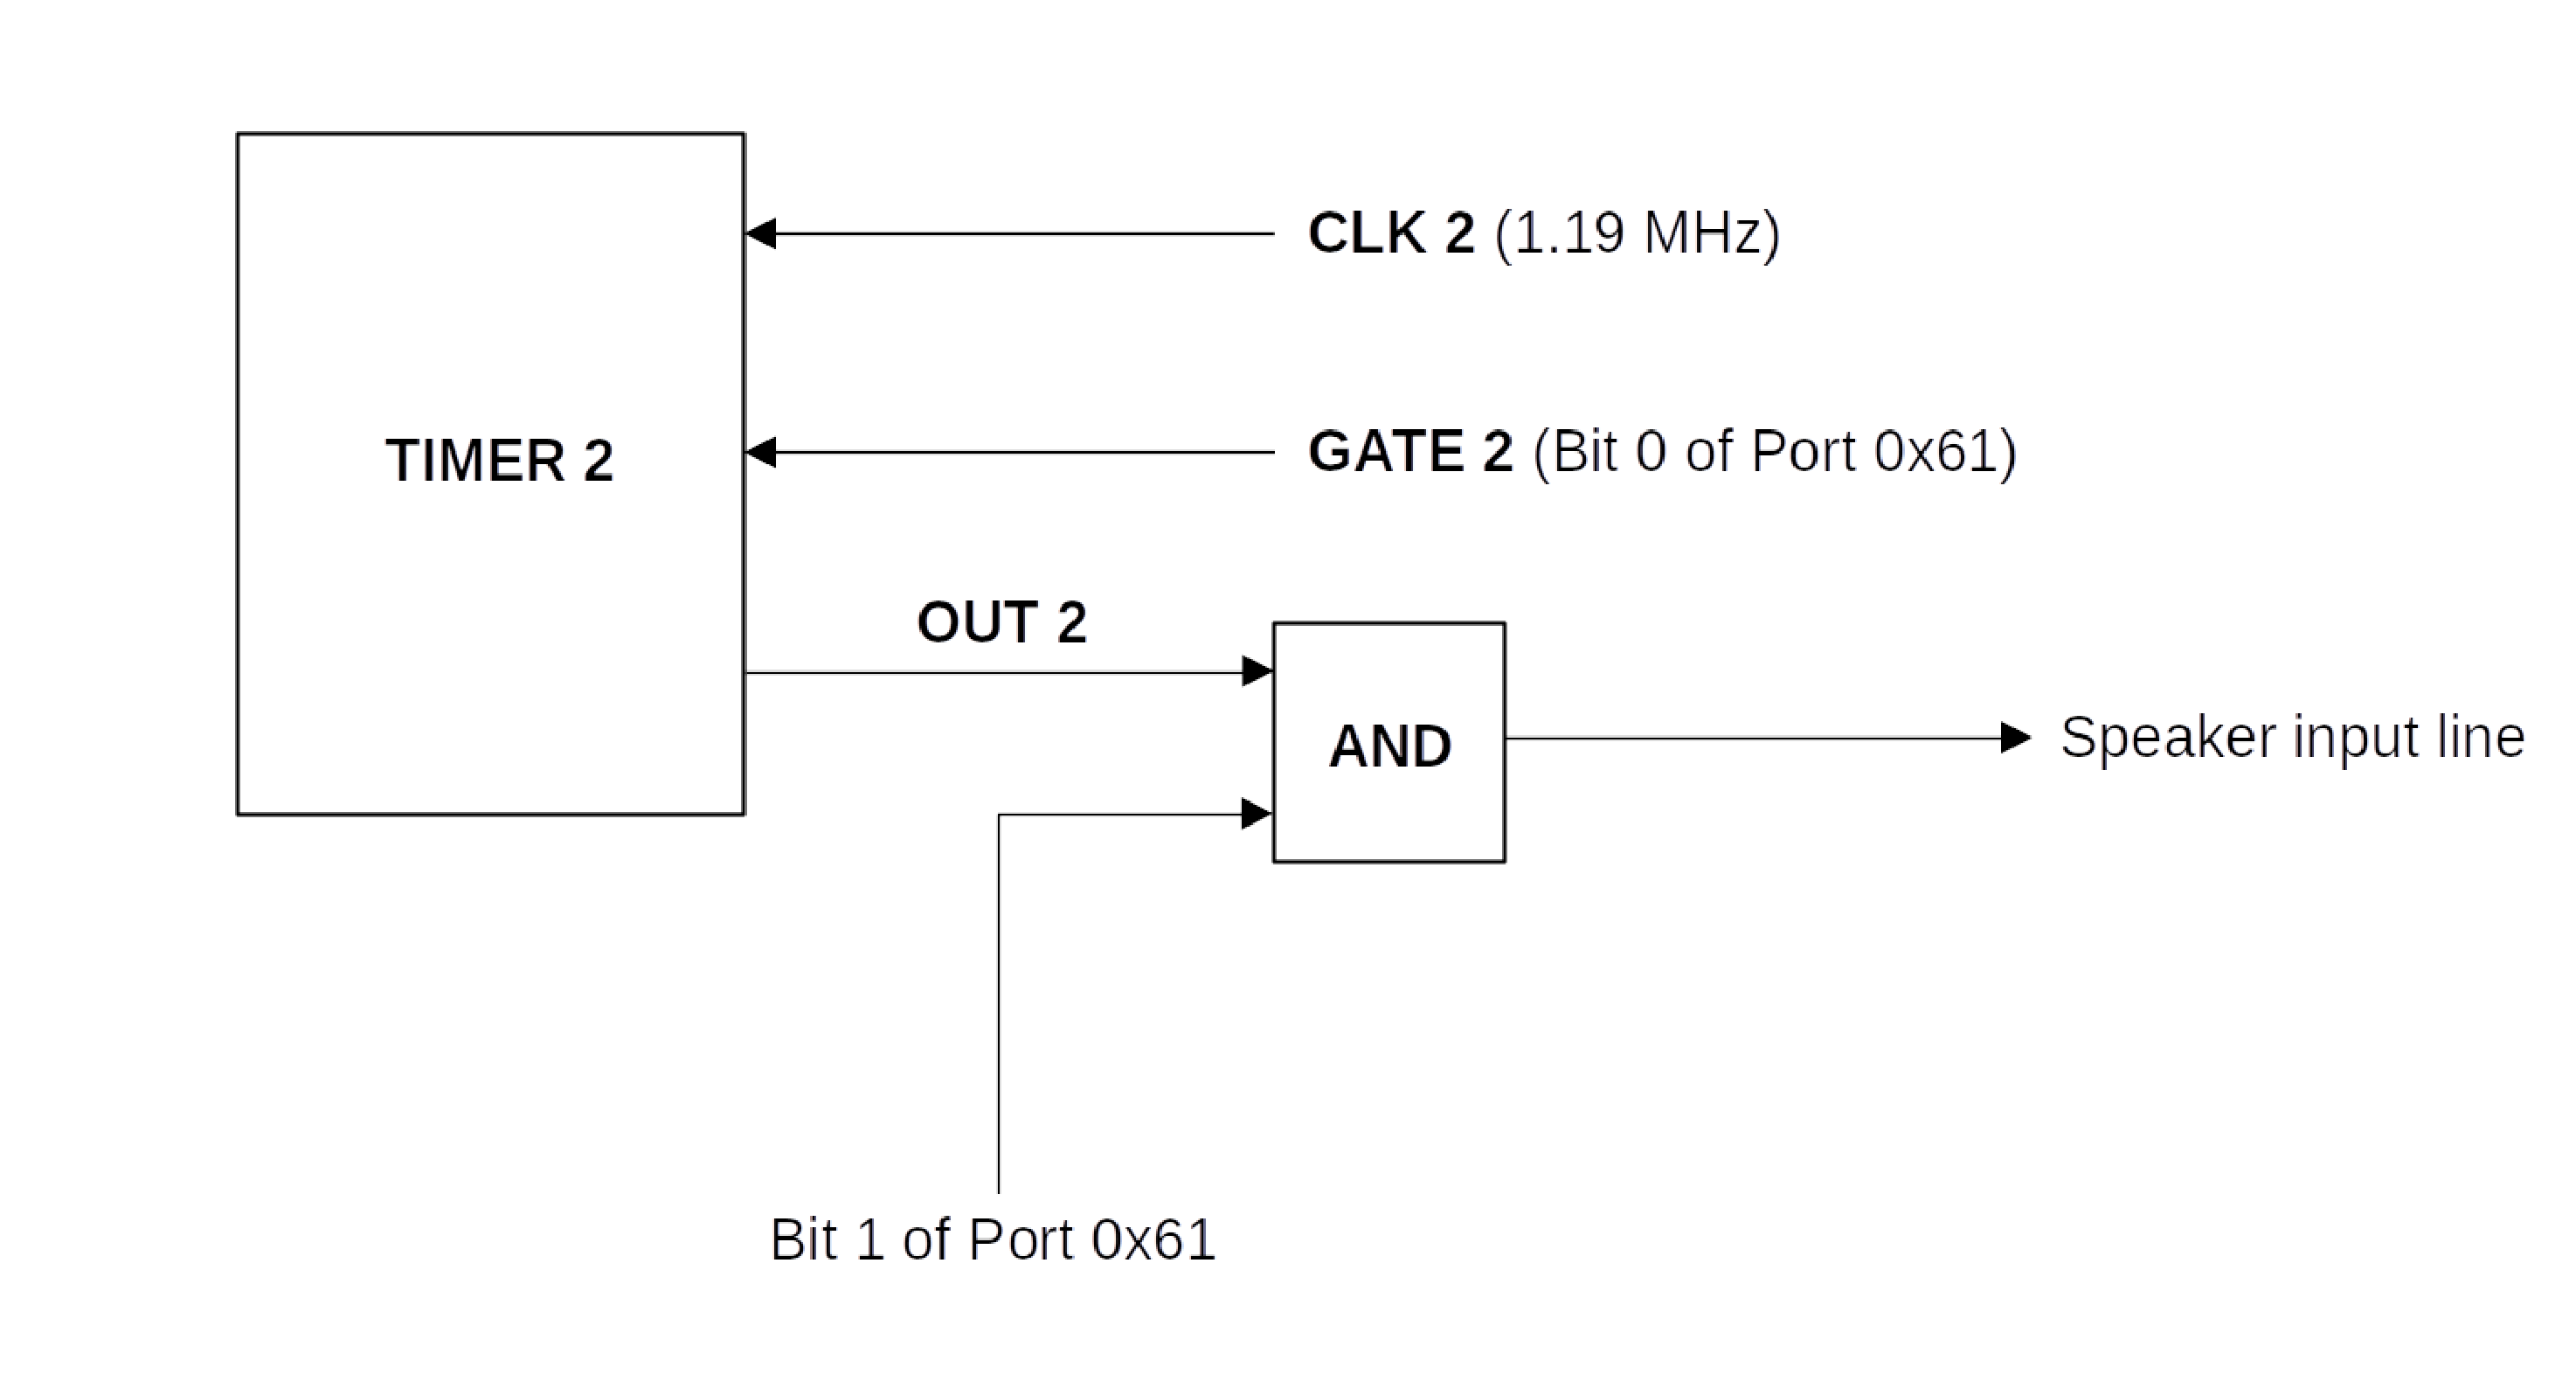
\includegraphics[scale=0.25]{figures/speakermap.eps}
  \caption{Connection of motherboard speaker with timer 2 of the PIT chip}
\label{fig:speakermap}
\end{figure}

The algorithm for producing a sound from the speaker by generating a square wave of particular frequency from timer 2 is as follows:
\begin{steps}[leftmargin=2cm]
  \item Select the frequency, $f$, of the sound you wish to generate. 
  \item Compute the value to be stored in the counter using the following formula:
  \begin{center}
  Value to be stored in the the counter, $N = \frac{1.19 MHz}{f}$
  \end{center}
  \item Round of $N$ to the nearest integer.
  \item Output a byte to port 0x43 specifying that timer 2 is to be used as a square wave generator, with the value of latch count being transmitted in binary, LSB being transmitted first, and then MSB.
  \item Output the LSB of the latch count value to port 0x42.
  \item Output the MSB of the latch count value to port 0x42.
  \item Read the value at port 0x61, $I$.
  \item Set bit 0 and 1 of value $I$. i.e., 
  \begin{center}
  $I = 00000011b$ \texttt{|} $I$
  \end{center} 
  \item Output $I$ to port 0x61.
  \item Delay while the note plays.
  \item Read the value at port 0x61, $I$.
  \item Clear bit 0 and 1 of value $I$, i.e.,
  \begin{center}
  $I = 11111100$ \texttt{\&} $I$
  \end{center}
  \item Stop the timer by outputting $I$ to port 0x61.
\end{steps}
This algorithm is used by the subroutines in \texttt{sound.asm }. These subroutines are:
\begin{enumerate}
  \item \texttt{sound\_tiny}
  		\begin{enumerate}[align=parleft, labelsep=2cm, leftmargin=1.06in]
  		  \item[Input]: \texttt{ax} = latch count value,\newline\texttt{bx} = down-counter's initial value
  		  \item[Output]: Nothing
  		  \item[Description]: Generates a sound wave equal to \texttt{ax}$\times 1.19 MHz$. Delay is provided by counting down from the value present in \texttt{bx}.
  		\end{enumerate}
  \item \texttt{sound\_mega}
  		\begin{enumerate}[align=parleft, labelsep=2cm, leftmargin=1.06in]
  		  \item[Input]: \texttt{ax} = latch count value,\newline\texttt{bx} = \texttt{sound\_tiny}'s down-counter's initial value,\newline\texttt{dx} = \texttt{sound\_mega}'s down-counter's initial value
  		  \item[Output]: Nothing
  		  \item[Description]: Generates a sound wave equal to \texttt{ax}$\times 1.19 MHz$ for a longer duration by using two nested down-counters.
  		\end{enumerate}
\end{enumerate}

\subsection{Disk Read/Write Operations: ..include/disk}
Disk read-write operations are necessary because they allow the user to store their data in a storage media which retains information even after the computer has been turned off. CrazyOS is capable of performing disk operations on floppy disks using INT 13 BIOS call. The core subroutines for checking a disks status and reading from, and writing to sectors on the disk are in \texttt{disk.asm} file. These subroutines are now described. 
\begin{enumerate}
  \item \texttt{disk\_status}
  		\begin{enumerate}[align=parleft, labelsep=2cm, leftmargin=1.06in]
  		  \item[Input]: Nothing
  		  \item[Output]: Nothing
  		  \item[Description]: Reads the status of last disk operation using INT 13,01 BIOS call. Disk status is returned as an 8-bit number in \texttt{al}. Each number corresponds to a particular event. For example, if \texttt{al} = 0x00, then the previous disk operation was successful. If \texttt{al} = 0x01, then an invalid parameter was passed in \texttt{ah} or other registers, and so on. These messages are printed by a call to \texttt{print\_disk\_status} after executing the BIOS call.
  		\end{enumerate}
  \item \texttt{disk\_read}
  		\begin{enumerate}[align=parleft, labelsep=2cm, leftmargin=1.06in]
  		  \item[Input]: \texttt{al} = number of sectors to be read,\newline\texttt{ch} = cylinder number,\newline\texttt{cl} = sector number,\newline\texttt{dh} = head number,\newline\texttt{dl} = drive number,\newline\texttt{es:bx} = segment:offset
  		  \item[Output]: Nothing
  		  \item[Description]: Reads sectors from a disk using INT 13,02 with the parameters that have been passed to it. Sectors are read and their contents are stored at address \texttt{es:bx}. In case the carry bit is set after disk read, \texttt{disk\_status} is called to print the error message.
  		\end{enumerate}
  \item \texttt{disk\_write}
  		\begin{enumerate}[align=parleft, labelsep=2cm, leftmargin=1.06in]
  		  \item[Input]: \texttt{al} = number of sectors to be written,\newline\texttt{ch} = cylinder number,\newline\texttt{cl} = sector number,\newline\texttt{dh} = head number,\newline\texttt{dl} = drive number,\newline\texttt{es:bx} = segment:offset
  		  \item[Output]: Nothing
  		  \item[Description]: Writes the content at address \texttt{es:bx} to the disk using INT 13,03 with the parameters that have been passed to it. In case the carry bit is set after disk write, \texttt{disk\_status} is called to print the error message.
  		\end{enumerate}
\end{enumerate}

The user does not need to hardcode the operating system to load his disk applications: he can simply use \texttt{disk read} command to load the application from a disk to a segment of his choice. Similarly, the user can write a segment to disk using \texttt{disk write} command in the shell. The subroutines which are executed when disk related commands are entered in the shell are present in \texttt{disk\_com.asm}. The primary subroutine which is executed when upon entering \texttt{disk} command in the shell is \texttt{disk\_com}. It is described below:
\begin{enumerate}
  \item[] \texttt{disk\_com}
  		\begin{enumerate}[align=parleft, labelsep=2cm, leftmargin=1.06in]
  		  \item[Input]: \texttt{si} = pointer to the first argument of \texttt{disk} command
  		  \item[Output]: Nothing
  		  \item[Description]: Executed when \texttt{disk} command is entered in the shell. Valid disk commands are \texttt{disk read}, \texttt{disk write}, and \texttt{disk -h}. Commands other than these generate an error message. Parameters for disk read/write operations are filled by \texttt{disk\_rw\_parameter\_fill} subroutine.
  		\end{enumerate}
\end{enumerate}

\subsection{APM Support: ../include/apm}
To control the power source of computers, vendors release various software packages which monitor and control the power source and power requirements of different computer peripherals. There are two main technologies used for putting power management in the hands of the operating system: Advanced Power Management (APM), and Advanced Configuration and Power Interface (ACPI). APM is a relatively older technology. ACPI is being used in favour of APM. However, as APM is much simpler than ACPI, the author decided to use APM for managing system power in this project.\\
APM was developed by Intel and Microsoft back in 1992. It enables an operating system running on an IBM compatible PC to use INT 15,53 BIOS call to manage power \cite{apm199612}. Before accessing the services of APM, it should be made sure that the operating system has been switched to real mode and that APM is enabled for all the devices. The algorithm to enable APM is presented below:
\begin{steps}[leftmargin=2cm]
  \item Check whether APM is present or not. If APM is not present then terminated this algorithm.
  \item Disconnect every device from APM.
  \item Connect to the real mode interface for APM.
  \item Enable APM for all the devices.
\end{steps}
\texttt{APM\_REAL\_MODE\_ENABLE} present in \texttt{apm.asm} is an implementation of this algorithm. After this algorithm has been executed, services of the APM can be used using INT 15,53 BIOS call.
The subroutines present in \texttt{apm.asm} are now described:
\begin{enumerate}
  \item \texttt{APM\_SERVICE\_ROUTINE}
  		\begin{enumerate}[align=parleft, labelsep=2cm, leftmargin=1.06in]
  		  \item[Input]: Registers \texttt{al}, \texttt{bx}, \texttt{cx}, and \texttt{dx} must be properly initialized for a particular APM service \cite{apm199612}.
  		  \item[Output]: Values are returned in general purpose registers depending upon the service that has been used \cite{apm199612}.
  		  \item[Description]: Used for accessing services of APM using INT 15,53 BIOS call.
  		\end{enumerate}
  \item \texttt{APM\_REAL\_MODE\_ENABLE}
  		\begin{enumerate}[align=parleft, labelsep=2cm, leftmargin=1.06in]
  		  \item[Input]: Nothing
  		  \item[Output]: Nothing
  		  \item[Description]: Enables APM for all devices connecting to its real mode interface.
  		\end{enumerate}
  \item \texttt{APM\_POWER\_OFF\_ROUTINE}
  		\begin{enumerate}[align=parleft, labelsep=2cm, leftmargin=1.06in]
  		  \item[Input]: Nothing
  		  \item[Output]: Nothing
  		  \item[Description]: Powers off the system provided APM is present.
  		\end{enumerate}
  \item \texttt{APM\_POWER\_LEVEL\_ROUTINE}
  		\begin{enumerate}[align=parleft, labelsep=2cm, leftmargin=1.06in]
  		  \item[Input]: Nothing
  		  \item[Output]: Nothing
  		  \item[Description]: Prints the power level of the system. At present not function on qemu-system-i386.
  		\end{enumerate}
\end{enumerate}
\texttt{apm\_com.asm} contains a single subroutine, \texttt{power\_com} which is executed when \texttt{power} command is entered in the shell. Its description is given below:
\begin{enumerate}
  \item[] \texttt{power\_com}
  		\begin{enumerate}[align=parleft, labelsep=2cm, leftmargin=1.06in]
  		  \item[Input]: \texttt{si} = pointer to the first argument of \texttt{power} command
  		  \item[Output]: Nothing
  		  \item[Description]: Processes the arguments passed with \texttt{power} command. Supported arguments/options are:
  		  \begin{enumerate}
  		  \item[]\texttt{off}: Used for turning the computer off, provided it supports APM
  		  \item[]\texttt{level}: Used for checking the charge left in the battery. Currently prints "Power level unknown".
  		  \item[]\texttt{-h}: Used for displaying valid options to be passed with \texttt{power} command.
		\end{enumerate}
  		\end{enumerate}
\end{enumerate}

\section{Applications}
Early in the development of this project, the author read that an assembler, a line editor, and a shell formed the first three applications for the UNIX operating system. This inspired him to write a shell and a line editor for CrazyOS. The idea of developing an assembler was dropped because of time constraints.\\
The applications for CrazyOS can be divided into two categories: system applications and user applications. Those applications which are ran from the shell and have been included on the same disk as the operating system itself are called system applications. Those applications which the programmer writes and loads on the second floppy disk are called user applications or disk applications. System application files are in the \texttt{../apps} directory (\autoref{fig:dirtapps}), and disk applications are in the \texttt(../disk-apps) directory (\autoref{fig:dirtreecrazyos86}). As of writing of this report, there are two system applications, namely, the shell and the line editor. There is only a single user application, the sound and light program, \texttt{soundnlight.asm}. In this section, we will first discuss the aforementioned system applications, starting with the shell. Then we will briefly discuss \texttt{soundnlight.asm}.
\begin{figure}[H]
\begin{forest}
  for tree={
    font=\ttfamily,
    grow'=0,
    child anchor=west,
    parent anchor=south,
    anchor=west,
    calign=first,
    edge path={
      \noexpand\path [draw, \forestoption{edge}]
      (!u.south west) +(7.5pt,0) |- node[fill,inner sep=1.25pt] {} (.child anchor)\forestoption{edge label};
    },
    before typesetting nodes={
      if n=1
        {insert before={[,phantom]}}
        {}
    },
    fit=band,
    before computing xy={l=15pt},
  }
[CrazyOS/8086/apps
  [edit
    [edit.asm]  
  ]
  [shell
    [cmdlist.asm]
    [shell.asm]
  ]
]
\end{forest}
\caption{Directory tree for \texttt{CrazyOS/8086/apps} (depth = 1)}
\label{fig:dirtapps}
\end{figure}

\subsection{Shell: ../apps/shell}
The shell is considered as the \textit{mother of all programs}. It is one of the first programs which runs in most operating systems. It provides the user an environment where he can issue commands and run other programs \cite{torvalds2001just}. The environment provided to the user in which he can write using a keyboard and see the characters on the screen is called a \textit{terminal emulator} as it emulates the old teletype-writers such as ASR Model 33. In CrazyOS, the terminal emulator is implemented by the use of subroutines present in \texttt{../include/ttyio} directory, in particular by \texttt{getline} and \texttt{printf} subroutines. The shell is implemented by the source code present in \texttt{../apps/shell} directory. This directory contains two source files: \texttt{shell.asm} and \texttt{cmdlist.asm}. There is only a single subroutine present in \texttt{shell.asm}, \texttt{main}. This subroutine firstly prints the prompt, \texttt{>}, using \texttt{printf}. Then it calls \texttt{getline} subroutine which takes input from the keyboard until the enter key gets pressed. Then using a blank space as the token separator, \texttt{lexer} splits the line into command word and arguments which are then executed.\\
The commands which are supported by the shell are present in \texttt{cmdlist.asm}. \texttt{com} string is compared with the strings present in this file one by one until a match is found. If no match has been found then an error message is printed on the screen. The commands which are supported at the time of writing of this report are:
\begin{enumerate}
  \item \texttt{clear}
  		\begin{enumerate}[align=parleft, labelsep=2cm, leftmargin=1.06in]
  		  \item[Description]: Clears the screen and displays prompt on the first line.
  		\end{enumerate}
  \item \texttt{date}
  		\begin{enumerate}[align=parleft, labelsep=2cm, leftmargin=1.06in]
  		  \item[Description]: Displays current date in \texttt{WEEKDAY, DD-MM-YY} format.
  		\end{enumerate}
  \item \texttt{disk}
  		\begin{enumerate}[align=parleft, labelsep=2cm, leftmargin=1.06in]
  		  \item[Description]: Used for performing disk operations using INT 13 BIOS call.
  		  \item[Options]:
  		  \item[\texttt{-h}] Display available options.
  		  \item[\texttt{read}] Format: \texttt{read D:C:H:S SEG:OFF N}.\\Read \texttt{N} sectors from the disk no. \texttt{D} starting with cylinder \texttt{C}, head \texttt{H}, and sector \texttt{S}. Contents are stored at \texttt{SEG:OFF}.
  		  \item[\texttt{status}] Display status of last disk operation.
  		  \item[\texttt{write}] Format: \texttt{write D:C:H:S SEG:OFF N}\\Write data at \texttt{SEG:OFF} to \texttt{N} sectors of disk \texttt{D} starting with cylinder \texttt{C}, head \texttt{H}, and sector \texttt{S}.
  		  \item[Note] \texttt{D} = drive no. (decimal),\newline\texttt{C} = Cylinder no. (decimal),\newline\texttt{H} = Head no. (decimal),\newline\texttt{S} = Sector no. (decimal),\newline\texttt{SEG} = 16-bit segment base address (hexadecimal),\newline\texttt{OFF} = 16-bit offset from segment base address (hexadecimal),\newline\texttt{N} = No. of sectors to be read (decimal)    
  		\end{enumerate}
  \item \texttt{edit}
  		\begin{enumerate}[align=parleft, labelsep=2cm, leftmargin=1.06in]
  		  \item[Description]: Runs the line editor. Used for editing the contents of the buffer which has been passed as an argument.
  		  \item[Options]:
  		  \item[\texttt{SEG:OFF}] Address of the buffer in whose contents will be edited. \texttt{SEG} is the 16-bit segment base address. \texttt{OFF} is the 16-bit offset. Both are hexadecimal numbers.  
  		\end{enumerate}
  \item \texttt{power}
  		\begin{enumerate}[align=parleft, labelsep=2cm, leftmargin=1.06in]
  		  \item[Description]: Uses APM to perform power management.
  		  \item[Options]:
  		  \item[\texttt{-h}] Displays options available with \texttt{power} command.
  		  \item[\texttt{level}] Displays current power level.
  		  \item[\texttt{off}] Turns of the computer/emulator.
  		\end{enumerate}
  \item \texttt{run}
  		\begin{enumerate}[align=parleft, labelsep=2cm, leftmargin=1.06in]
  		  \item[Description]: Performs a far call to the memory address passed in the command.
  		  \item[Options]:
  		  \item[\texttt{SEG:OFF}]\texttt{SEG} = Segment base address (hexadecimal),\newline\texttt{OFF} = Offset (hexadecimal)
  		\end{enumerate}
  \item \texttt{srng}
  		\begin{enumerate}[align=parleft, labelsep=2cm, leftmargin=1.06in]
  		  \item[Description]: Displays a 16-bit positive random number.
  		\end{enumerate}
  \item \texttt{time}
  		\begin{enumerate}[align=parleft, labelsep=2cm, leftmargin=1.06in]
  		  \item[Description]: Displays current time in \texttt{hh:mm:ss} (24-hour) format.
  		\end{enumerate}
\end{enumerate}

\subsection{Editor: ../apps/edit}
\texttt{edit} is a simple line editor which is provided with CrazyOS. This line editor has been inspired from the infamously terse \texttt{ed} line editor which is the standard editor on UNIX and UNIX like operating systems.\\
The line editor is started by typing \texttt{ed SEG:OFF} in the shell. Here, \texttt{SEG} is the 16-bit segment base address and \texttt{OFF} is the 16-bit offset from the base address at which the contents of file will be stored. Due to the use of segments, the size of the file cannot exceed 64 kiB or about 819 80-character wide lines. Also, each file is terminated with a magic number, 0xaa. This hex-number maps to \textit{á} in code page 437. As in this simple project we are not using accented letters, therefore, we do not have to worry about the loss of characters which might happen to exist in the file buffer after 0xaa.\\
Once the editor starts, the user is told about the number of characters that have been found in the file buffer. Like \texttt{ed}, \texttt{edit} allows the user to enter a single line at a time. The line so entered should not exceed 80 character limit. If the first character of the line is an asterisk, than the subsequent characters are considered as editor commands and are not stored in the file buffer. Valid editor commands are:
\begin{enumerate}
  \item \texttt{edit}
  		\begin{enumerate}[align=parleft, labelsep=2cm, leftmargin=1.06in]
  		  \item[Description]: Allows the user to edit a previous line.
  		  \item[Format]: \texttt{*edit N}, where \texttt{N} is a valid positive integer. 
  		\end{enumerate}
  \item \texttt{exit}
  		\begin{enumerate}[align=parleft, labelsep=2cm, leftmargin=1.06in]
  		  \item[Description]: Displays the number of sectors that will be required to fit the contents of the file and then exits from the editor.
  		  \item[Format]: \texttt{*exit}
  		\end{enumerate}
  \item \texttt{list}
  		\begin{enumerate}[align=parleft, labelsep=2cm, leftmargin=1.06in]
  		  \item[Description]: Lists the contents of the file.
  		  \item[Format]: \texttt{*list}
  		\end{enumerate}
\end{enumerate}
If an invalid command is passed to editor, then all the characters except for the asterisk will be saved in the file buffer.\\
The file can be saved permanently by using \texttt{disk write} command to write the buffer to the disk. 

\section{Disk Applications: ../disk-apps}
As we have discussed before, applications which come on a separate disk are called disk applications in this project. Source code for disk applications are saved at \texttt{../disk-apps} directory. At present, the whole project has only a single disk application, namely \texttt{soundnlight.asm}. This assembly file contains code which reads a single byte from the kernel (present in block 1), and
\begin{enumerate}
  \item displays a pixel having a color corresponding to the value of the byte that has been read using INT 10,0C BIOS call.
  \item generates a note corresponding the value of the byte that has just been read using \texttt{sound\_tiny} subroutine present in \texttt{../include/sound/sound.asm}.
\end{enumerate}
Then the pointer \texttt{si} is incremented and the next byte of the kernel is read. The screen is assumed to have a size of $640\times480$ pixels. Other available screen resolutions are $640\times350$ and $320\times200$ pixels.

\section{Building Binaries and Disk Images}
The phrase "building a project" in computer science refers to building an application or producing something which will be used in the for getting the task done. The final result is ran and tested. Many times the final result is not what was required which might require that certain files be removed. Typing all of these commands in the terminal to build and run the project and clean redundant files will be tedious. To automate this process we have used GNU Make automation software which allows us to do all of the aforementioned tasks with just a few simple commands.\\
In this project, we want disk images of two 3.5'' floppy disk having a size of 1.44 MiB. The first floppy disk will be having the binary of the bootloader and CrazyOS. The second floppy disk will be having the binary of our disk applications and will be used as a permanent storage media for storing files. Therefore, during clean up procedure, every binary file except for the second disk will be removed.\\
To build the binaries of the bootloader and the operating system, we type go to the project directory in the terminal and then type\\\texttt{make build}\\
This command builds the binaries of the bootloader and the operating system and concatenates them into 1.44 MiB file. Binaries of disk applications are also created and concatenated into another 1.44 MiB binary file. These files are produced using \texttt{../mkdisk1.asm} and \texttt{../mkdisk2.asm}, respectively. Both of these files use \texttt{times} directive we discussed in section 3.3.1. The first disk which contains the bootloader and the operating system has the name \texttt{CrazyOS.bin} and the second disk having the disk applications has the name \texttt{disk2.bin}. A file named \texttt{CrazyOS.img} is also created. It has the same contents as \texttt{CrazyOS.bin} and is created so that it can be used with emulators other than QEMU (such as PCem) which only support \texttt{.img} files.\\
The operating system is ran using \texttt{make run} command. In case the programmer needs to rebuild fresh disk image, he can type \texttt{make clean} in the terminal to delete all binary images in the \texttt{../8086/build} folder except for \texttt{asm.bin}, which is the binary image of \texttt{soundnlight.asm}, and \texttt{disk2.bin}, which might be containing some files which the programmer might have written using CrazyOS.
%%%%%%%%%%%%%%%%%%%%%%%%%%%%%%%%%%%%%%%%%%%%%%%%%%%%%%%%%%%%%%%
\newpage
\chapter{Results and Discussion}
\section{Introduction}
We have discussed the implementation of CrazyOS. However, discussing the implementations is not enough for the reader needs to get their hands dirty to understand this project. For this reason, in this chapter we will present the results of this project. These results are obtained by running the operating system in QEMU's emulation of a system based on i386 processor. We have discussed how various commands are used in the shell and present to the reader the only three known bugs known in the operating system at the time of writing of this report.

\section{Cloning \& Running CrazyOS}
Since its inception, CrazyOS's version control has been done using Git and the repository has been hosted on Github. To download the source files of the project on a local machine, the user must first install Git and generate SSH keys and link them with his account on Github. Once these preliminary tasks have been done, the user has to type the following command in a terminal to clone CrazyOS:
\begin{Verbatim}
$ git clone git@github.com:PraneetKapoor2619/CrazyOS.git
\end{Verbatim} 
The \$ should be ignored; it is just a standard way of telling readers that they should type the text ahead in a terminal.\\
Once the project has been cloned, the reader has to make sure that the version of CrazyOS that he uses has the short commit ID 1a17fa0. For this, the following command has to be entered in the terminal:
\begin{Verbatim}
$ git reset --hard 1a17fa0
\end{Verbatim}
To move to the project directory, the following command is executed:
\begin{Verbatim}
$ cd CrazyOS/8086/
\end{Verbatim}
Once in the project directory, the user must create a build directory by the following command:
\begin{Verbatim}
$ mkdir build
\end{Verbatim}
The binary files and the disk images are built using \texttt{make build} command. To run the operating system, type
\begin{Verbatim}
$ make run
\end{Verbatim}
To exit QEMU without powering off the emulator from CrazyOS's shell, just press \texttt{Ctrl + Alt + Q}. \texttt{build} directory is cleaned by using \texttt{make clean} command. To remove \texttt{asm.bin} and \texttt{disk2.bin} in the \texttt{build} directory, the following commands should be used:
\begin{Verbatim}
$ rm build/asm.bin build/disk2.bin
\end{Verbatim}

\section{Using the Shell}
Upon running the emulation, the user will be greeted with a startup screen showing a text message, and current time and date, as shown in \autoref{fig:startupscrn}).
\begin{figure}[H]
  \centering
  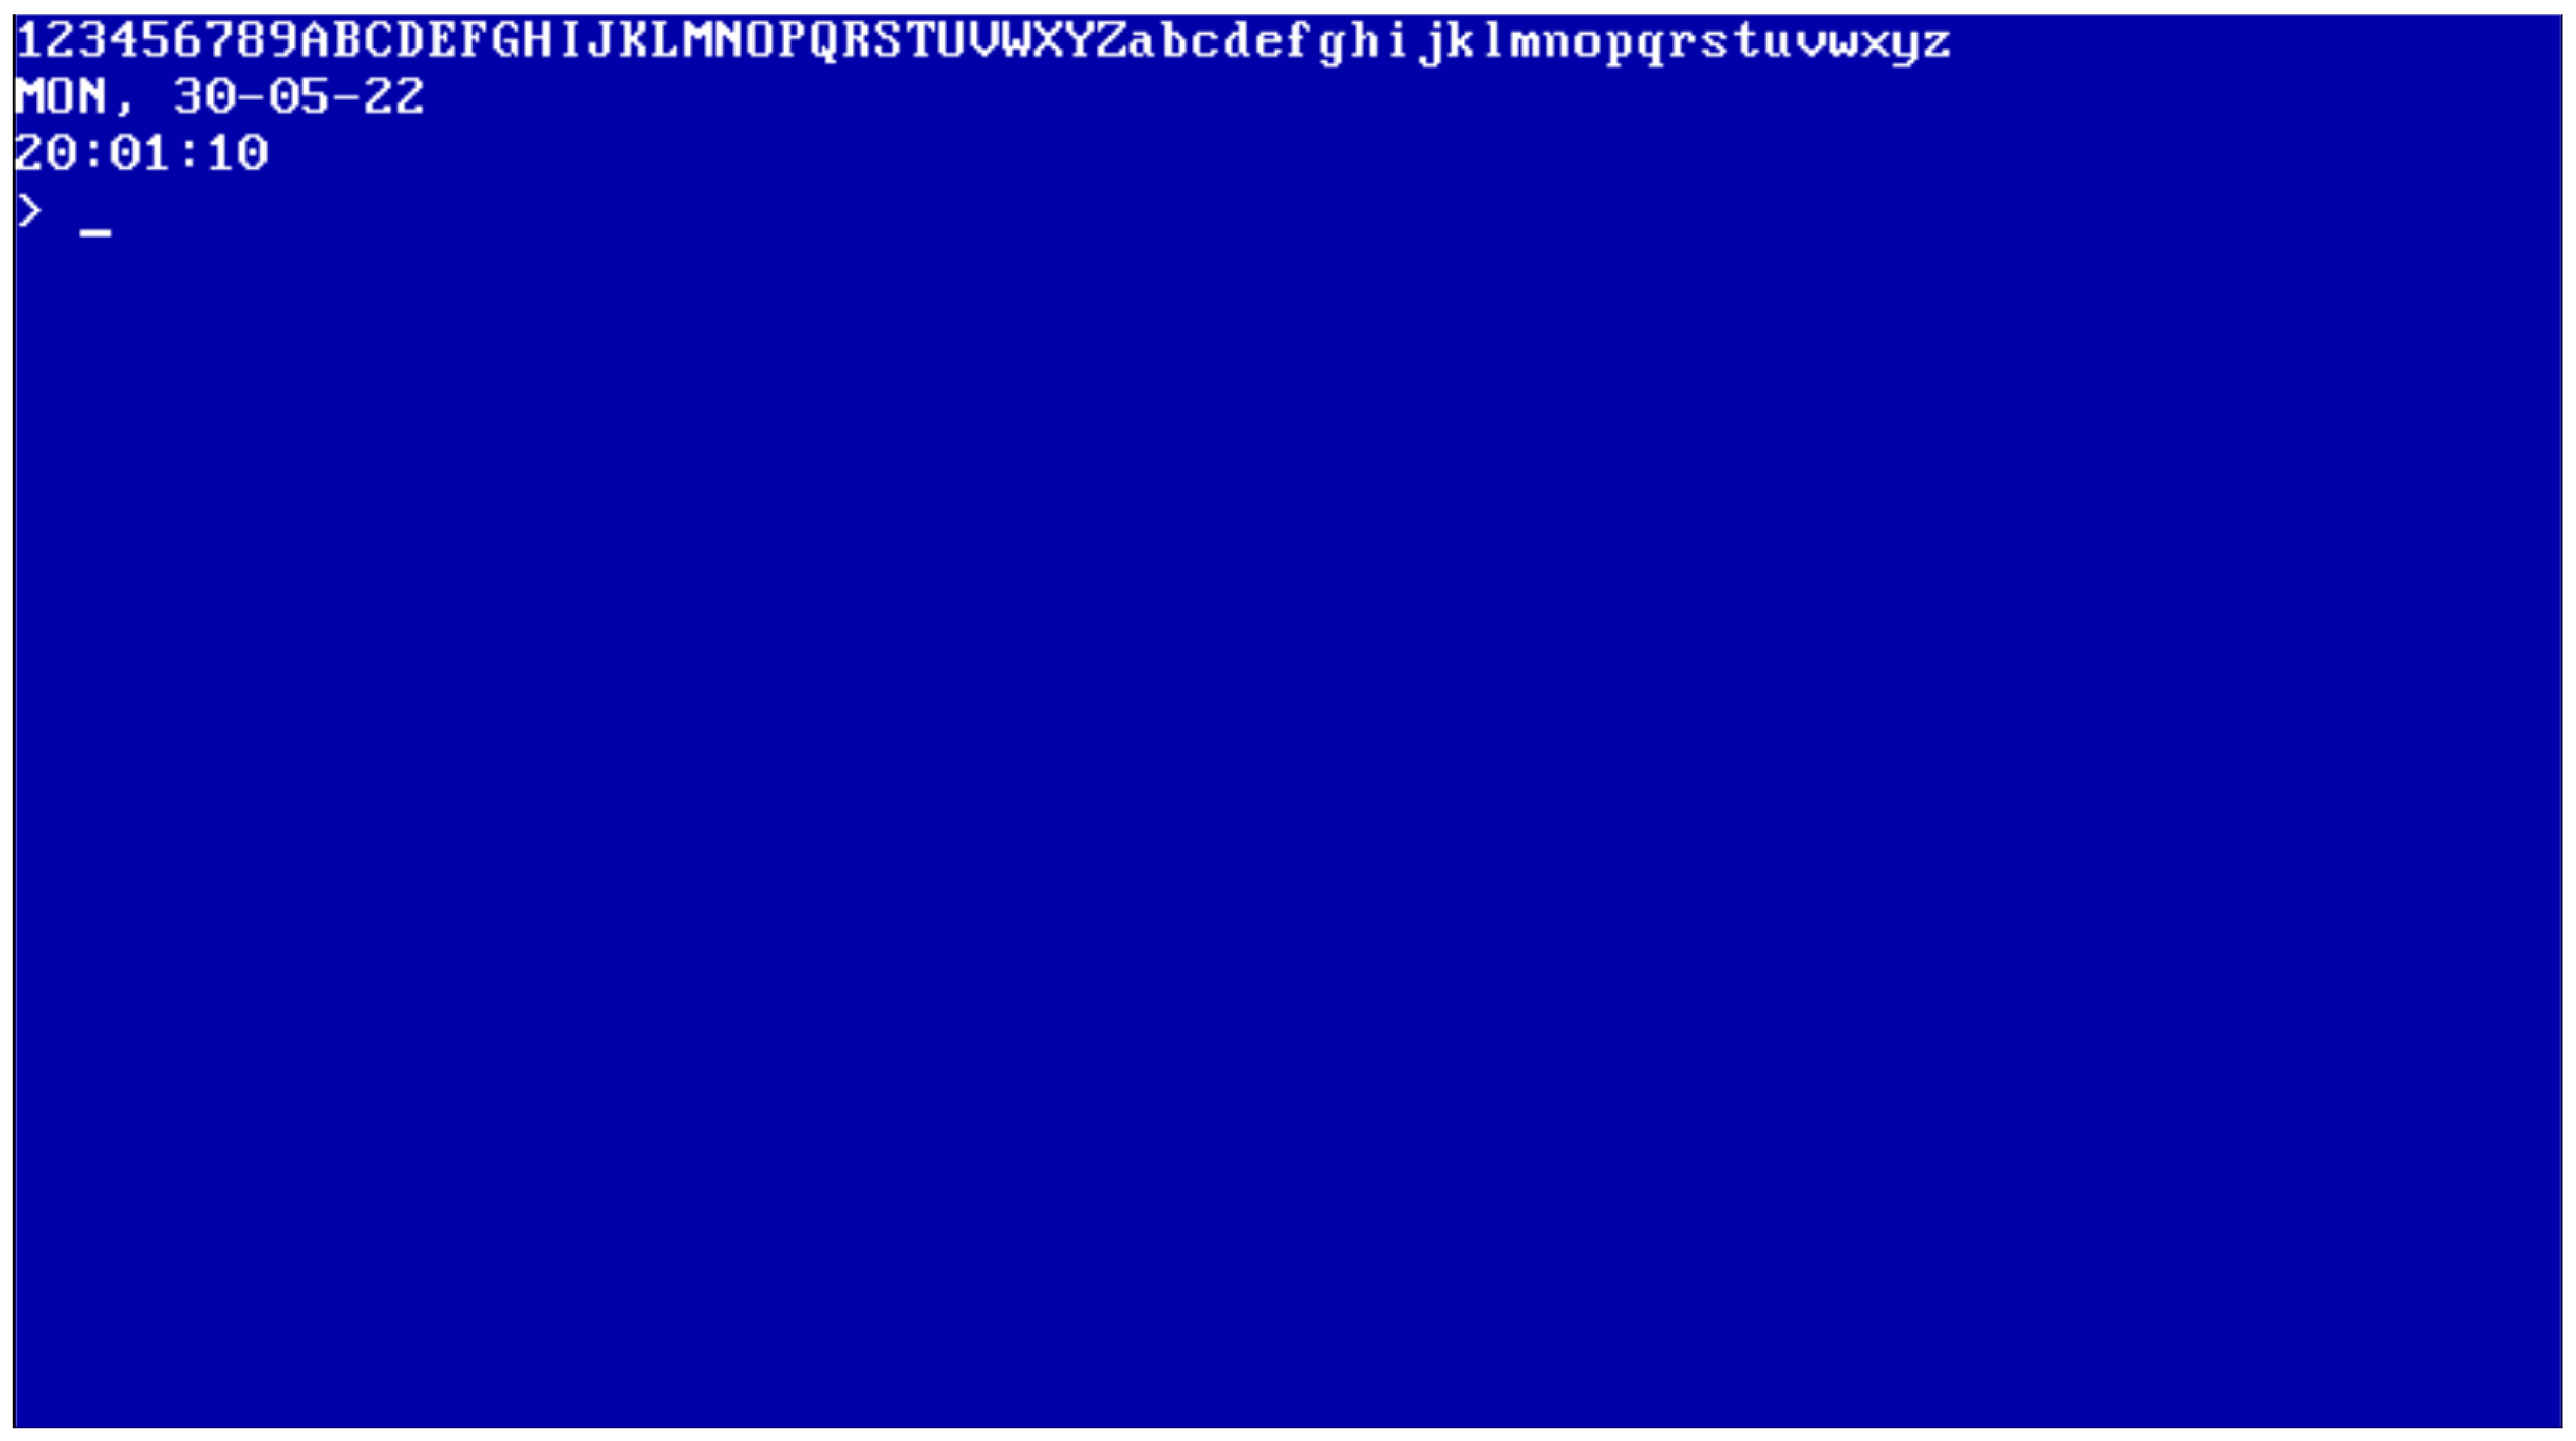
\includegraphics[scale=0.25]{figures/startupscrn.eps}
  \caption{CrazyOS startup screen}
\label{fig:startupscrn}
\end{figure}

\subsection{Using time, date, srng, and clear}
Using \texttt{time} and \texttt{date} command the user can know the current time and date, respectively. By typing \texttt{srng} multiple times, the user can generate different pseudo-random numbers. To clear the screen, \texttt{clear} command is used. Output of these commands are shown in \autoref{fig:timedatesrng}.
\begin{figure}[H]
  \begin{subfigure}{.5\textwidth}
  \centering
  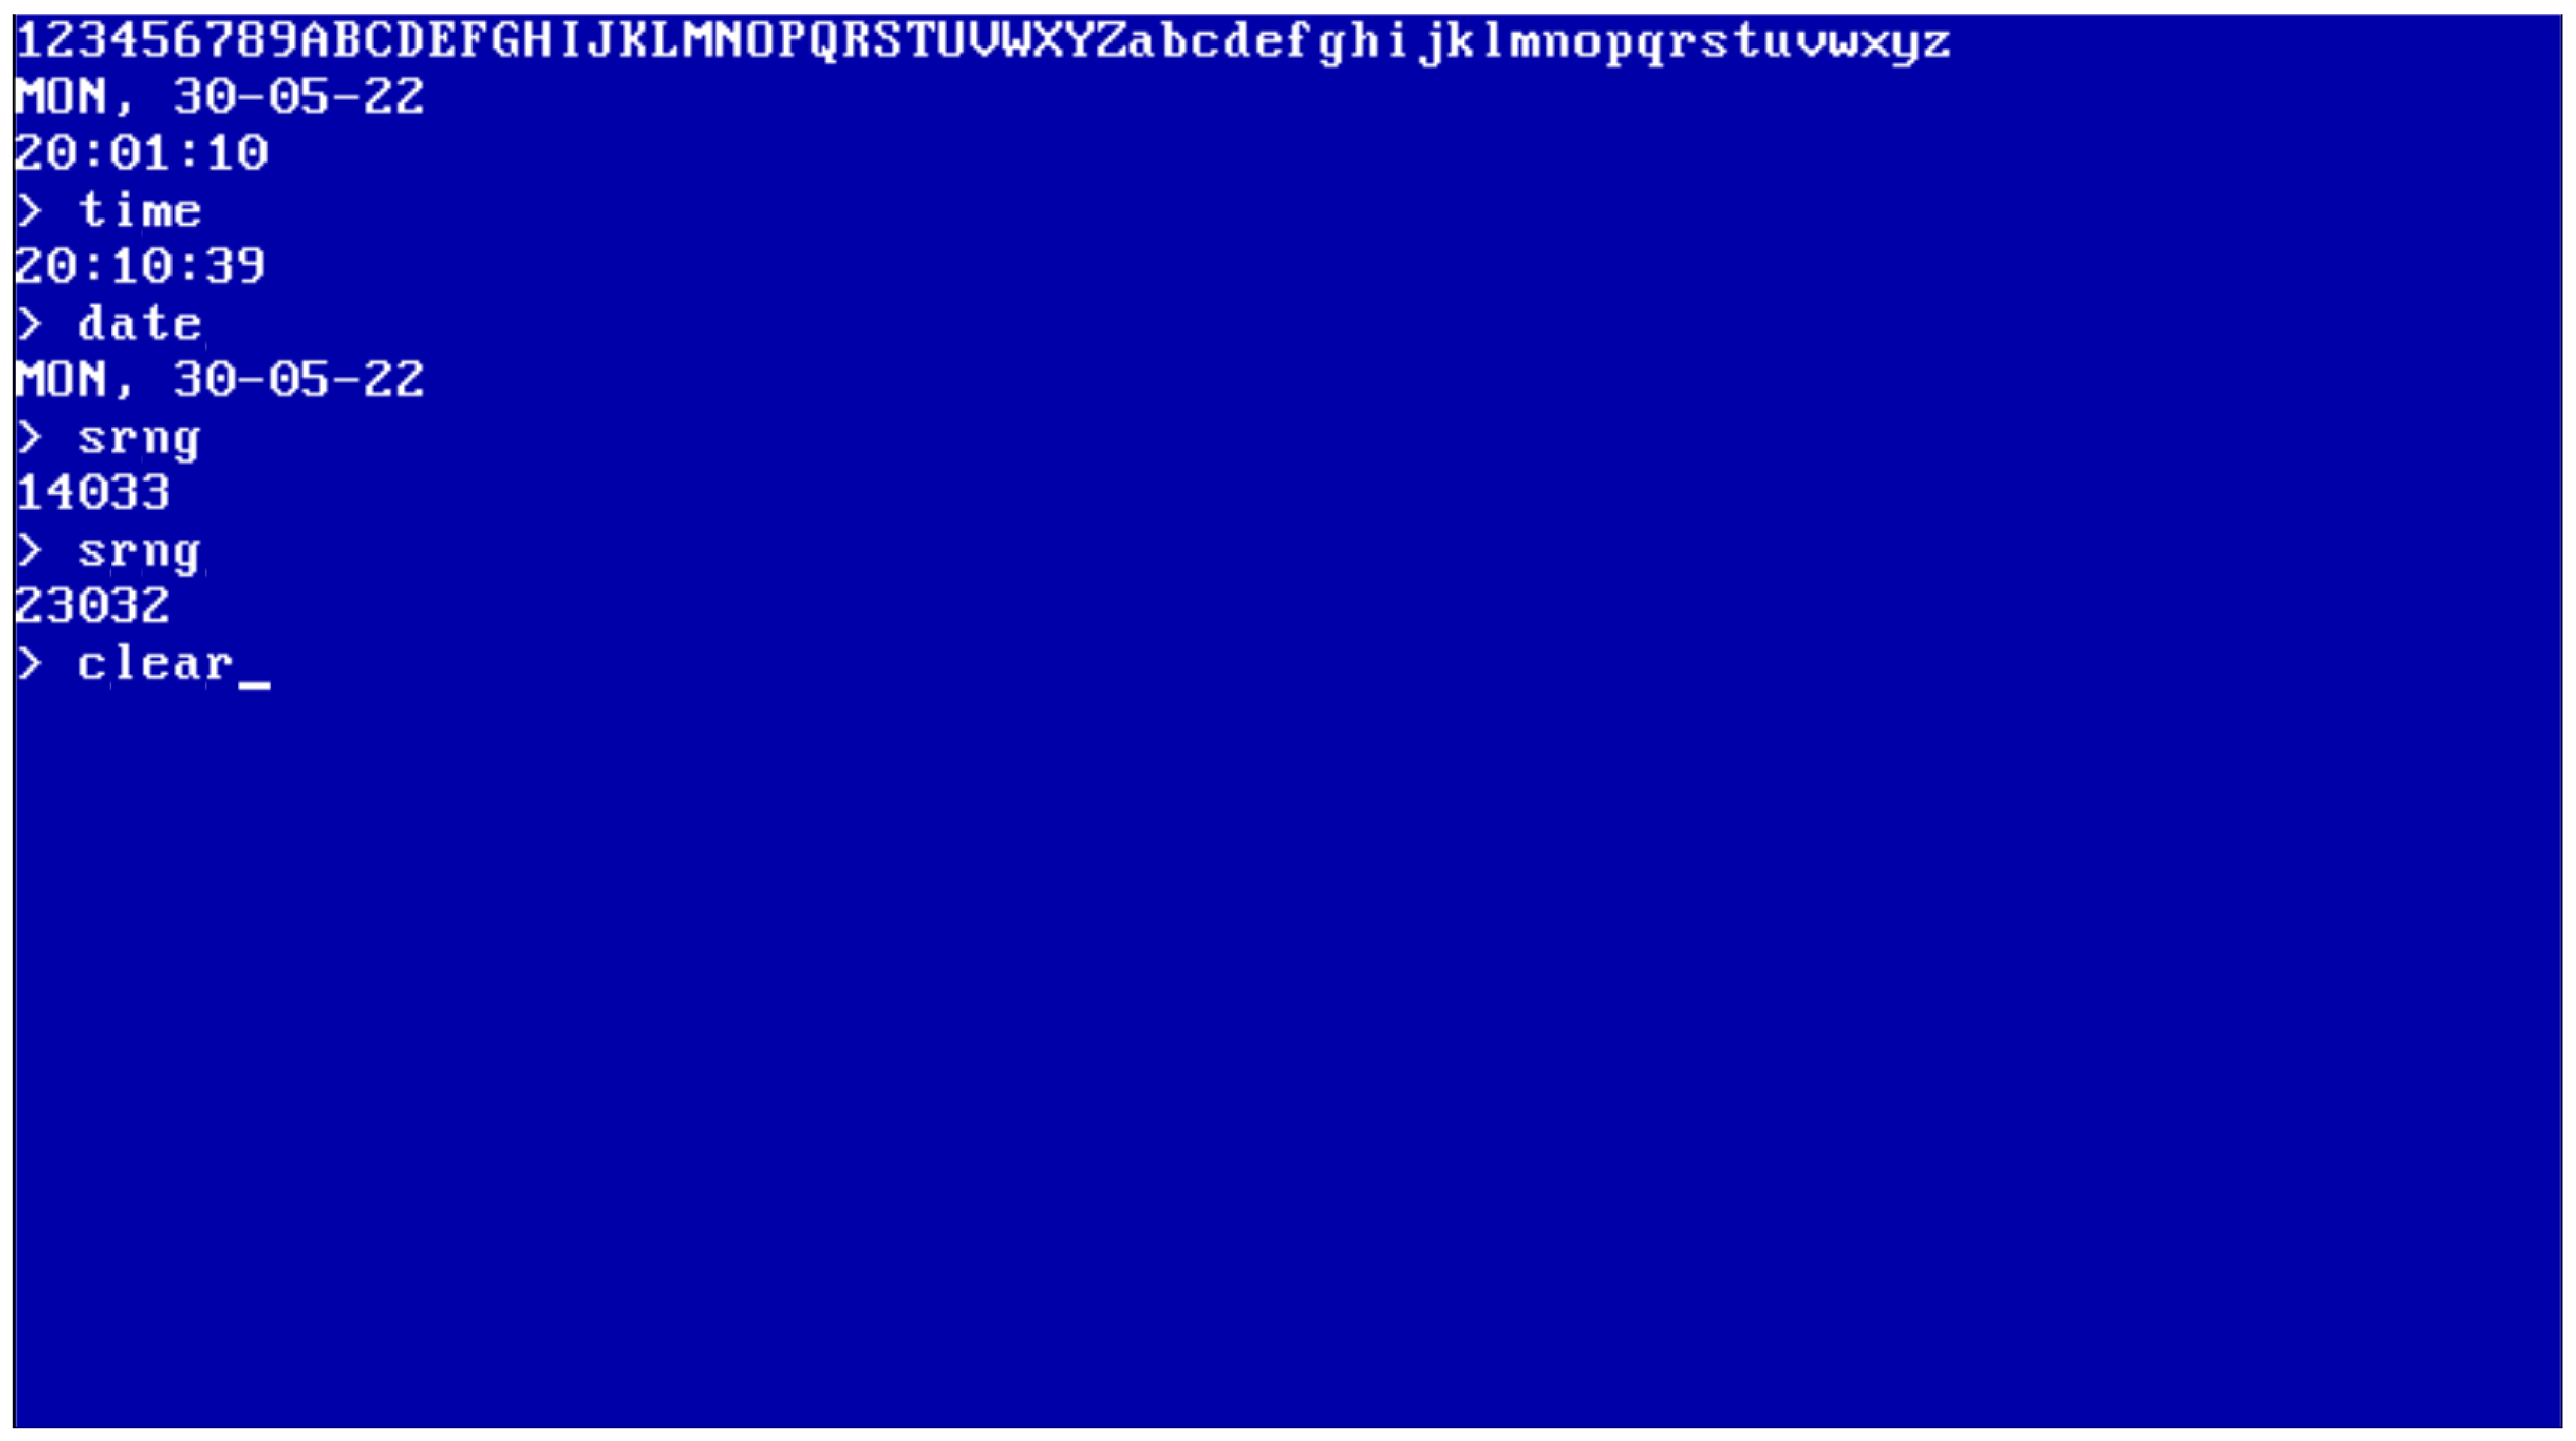
\includegraphics[scale=0.13]{figures/timedatesrng.eps}
  \caption{Using \texttt{time}, \texttt{date}, and \texttt{srng} commands}
  \end{subfigure}
  \begin{subfigure}{.5\textwidth}
  \centering
  
\includegraphics[scale=0.13]{figures/cleareffect.eps}
  \caption{Effect of \texttt{clear} command}
  \end{subfigure}
\caption{Using \texttt{time}, \texttt{date}, \texttt{srng}, and \texttt{clear} commands}
\label{fig:timedatesrng}
\end{figure}

\subsection{Running Disk Applications}
The binary of \texttt{../disk-apps/soundnlight.asm} is loaded at the first sector of \texttt{disk2.bin}. The application is first read using \texttt{disk read} command. In \autoref{fig:dskrdrun}, we have loaded the application in the 5th block. To run it, we type \texttt{run 5000:0000}. This performs an intersegment call and runs the application, thus producing coloured pixels and notes corresponding to the byte of the kernel that is being read, as shown in \autoref{fig:soundnlight}. As this application has no far return instruction, \texttt{retf}, we need to kill the emulation using \texttt{Ctrl + Alt + Q} key combo.
\begin{figure}[H]
  \begin{subfigure}{.5\textwidth}
  \centering
  
\includegraphics[scale=0.13]{figures/dskrdrun.eps}
  \caption{Using \texttt{disk read} and \texttt{run}}
  \label{fig:dskrdrun}
  \end{subfigure}
  \begin{subfigure}{.5\textwidth}
  \centering
  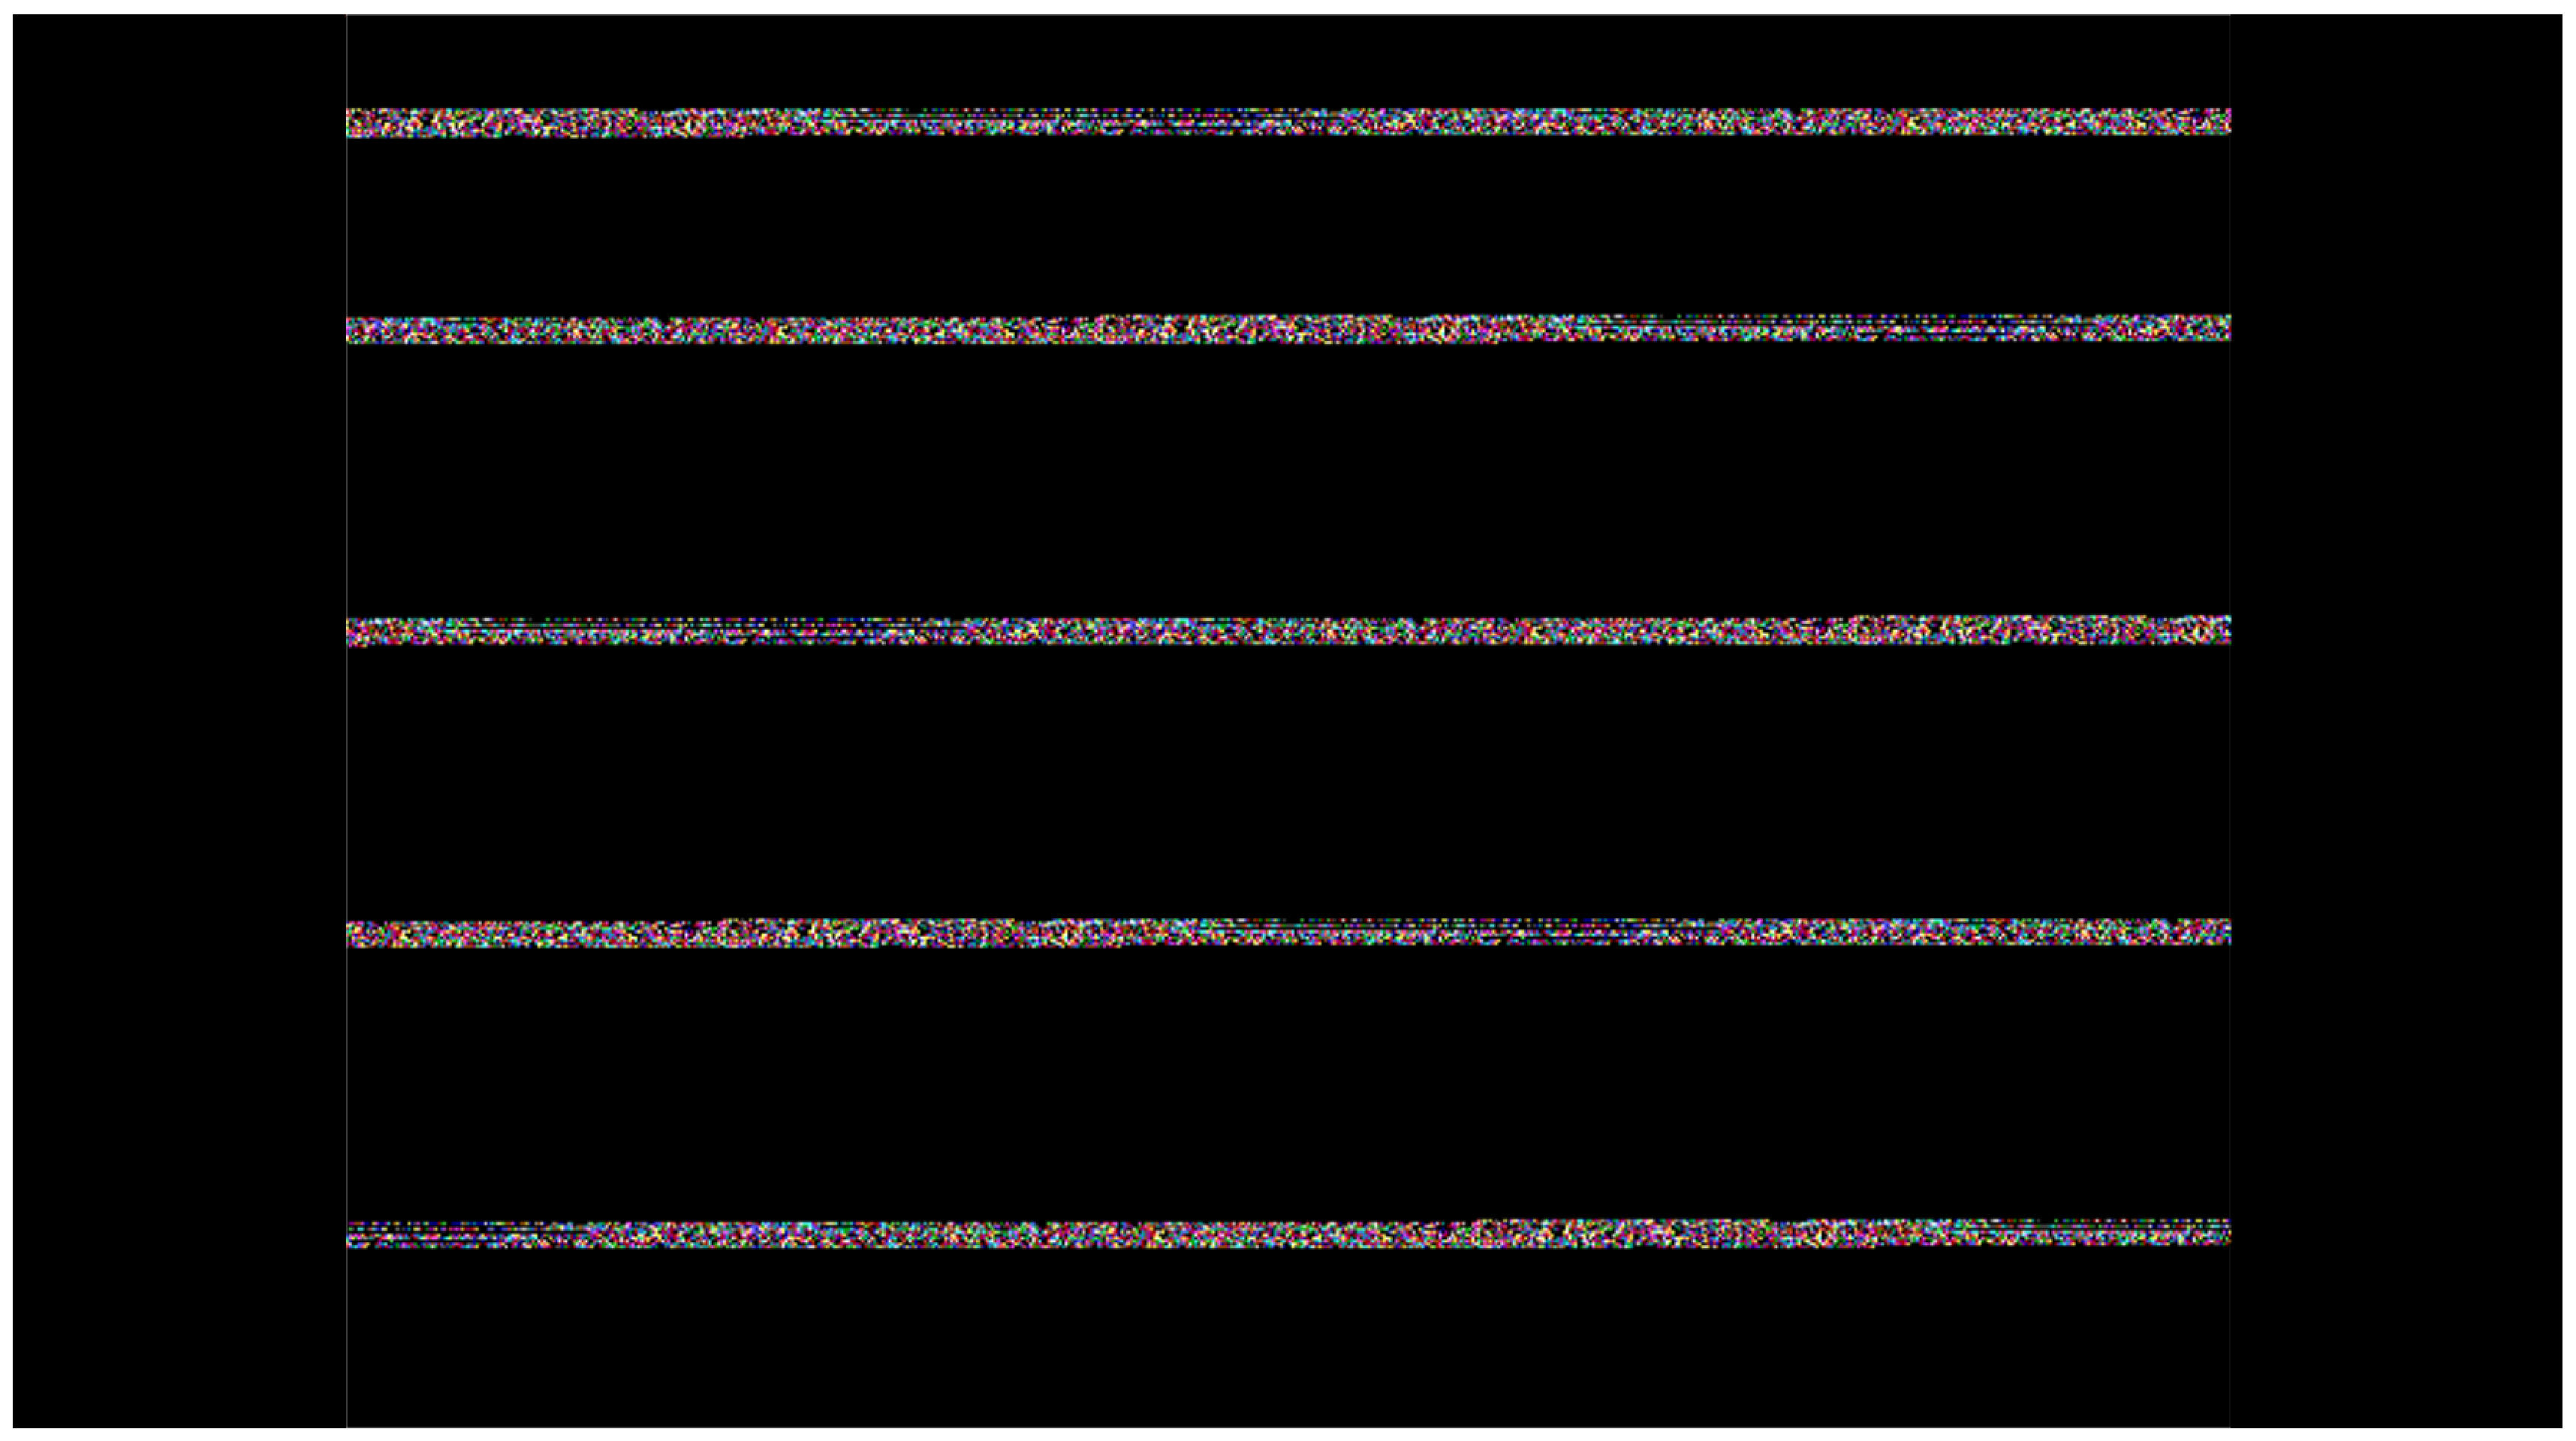
\includegraphics[scale=0.13]{figures/soundnlight.eps}
  \caption{Running \texttt{soundnlight}}
  \label{fig:soundnlight}  
  \end{subfigure}
\caption{Using \texttt{disk read} and \texttt{run} commands to run a disk application}
\end{figure}

\subsection{Power Commands}
\texttt{power} command is used to manage power of the machine using APM. Its use is shown in \autoref{fig:powercom}. Note that the command \texttt{power level} prints \texttt{Power level unknown}.
\begin{figure}[H]
  \centering
  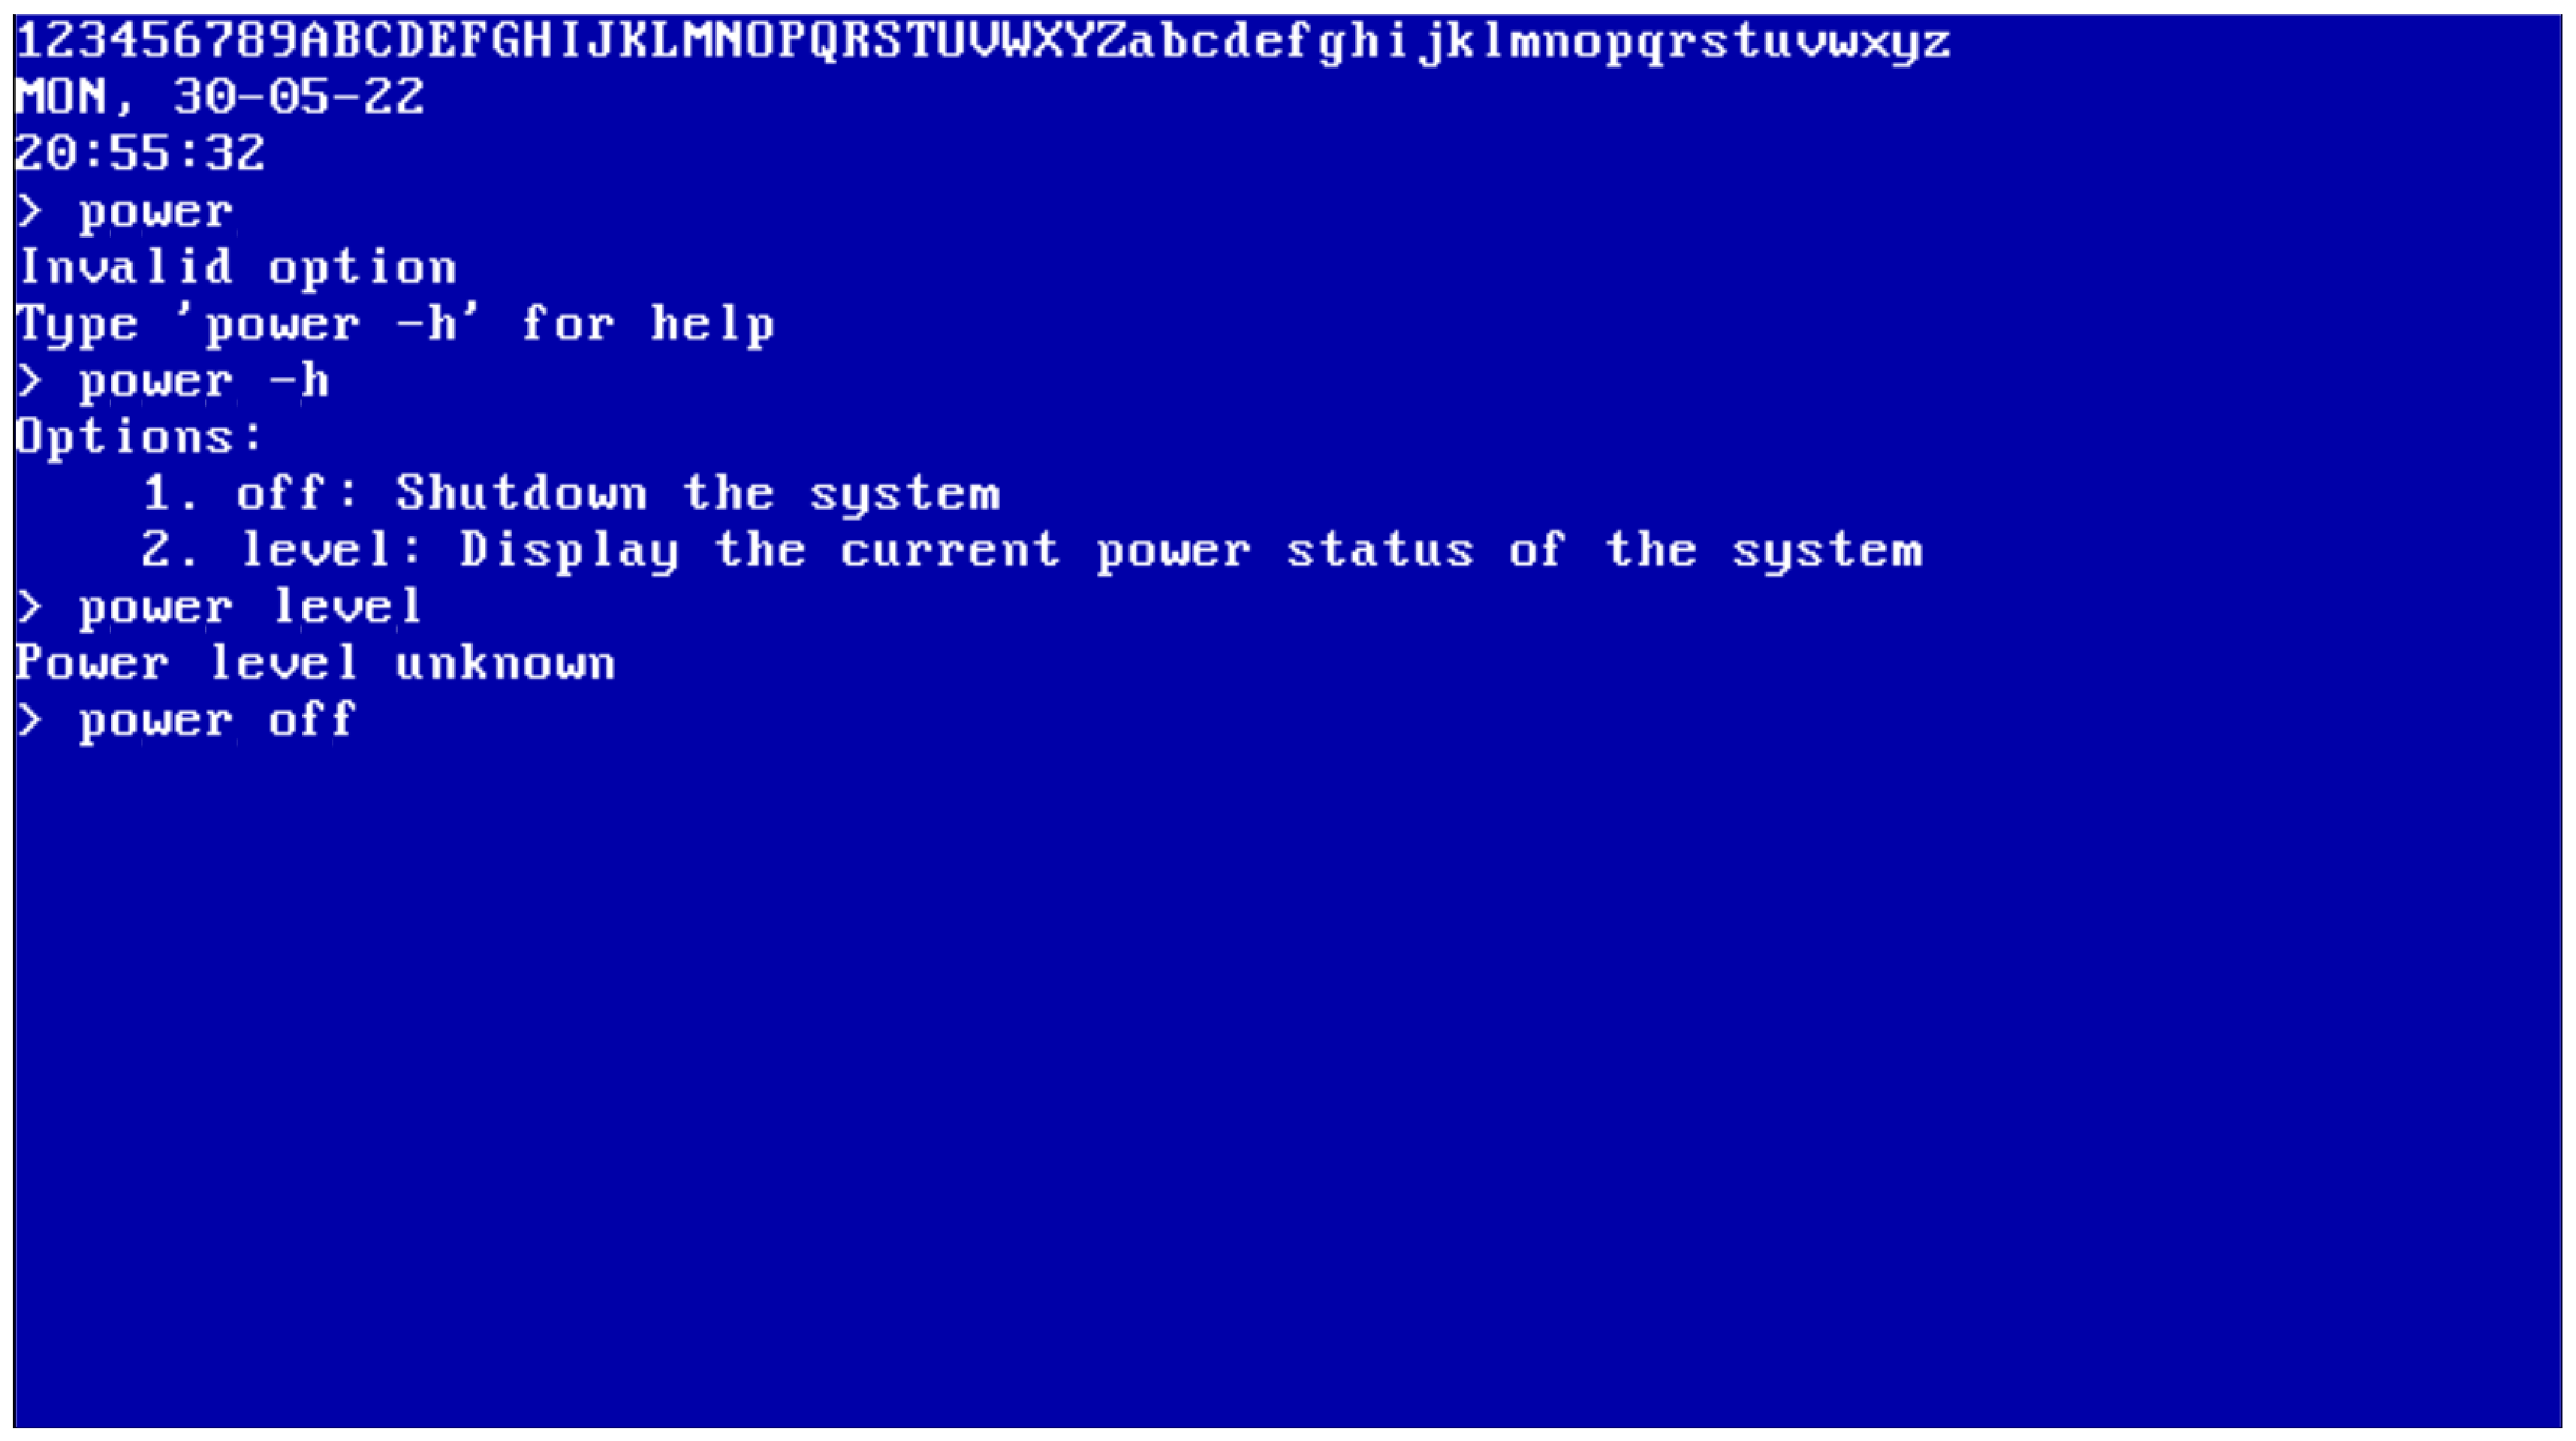
\includegraphics[scale=0.25]{figures/powercom.eps}
  \caption{Using \texttt{power} command}
\label{fig:powercom}
\end{figure}

\section{Using the Editor}
The line editor is ran from the shell by using the \texttt{edit} command. The address of the buffer should be passed as an argument. If the buffer is empty, then the total number of bytes is shown to be zero. Files are edited and their contents are listed using \texttt{*edit} and \texttt{*list} commands, respectively. Note that \texttt{*list} command clears the screen and then displays the contents of the buffer. To exit the editor, \texttt{*exit} command is used. Contents of the buffer are written to the disk using \texttt{disk write} command. \autoref{fig:editor1} shows these commands in action.\\
The same sectors of the disk to which we have written earlier can be read again and opened and listed in the editor. \autoref{fig:editor2} is a proof that the line editor and disk read/write commands are able to successfully able to create, save and edit files.
\begin{figure}[H]
  \begin{subfigure}{.5\textwidth}
  \centering
  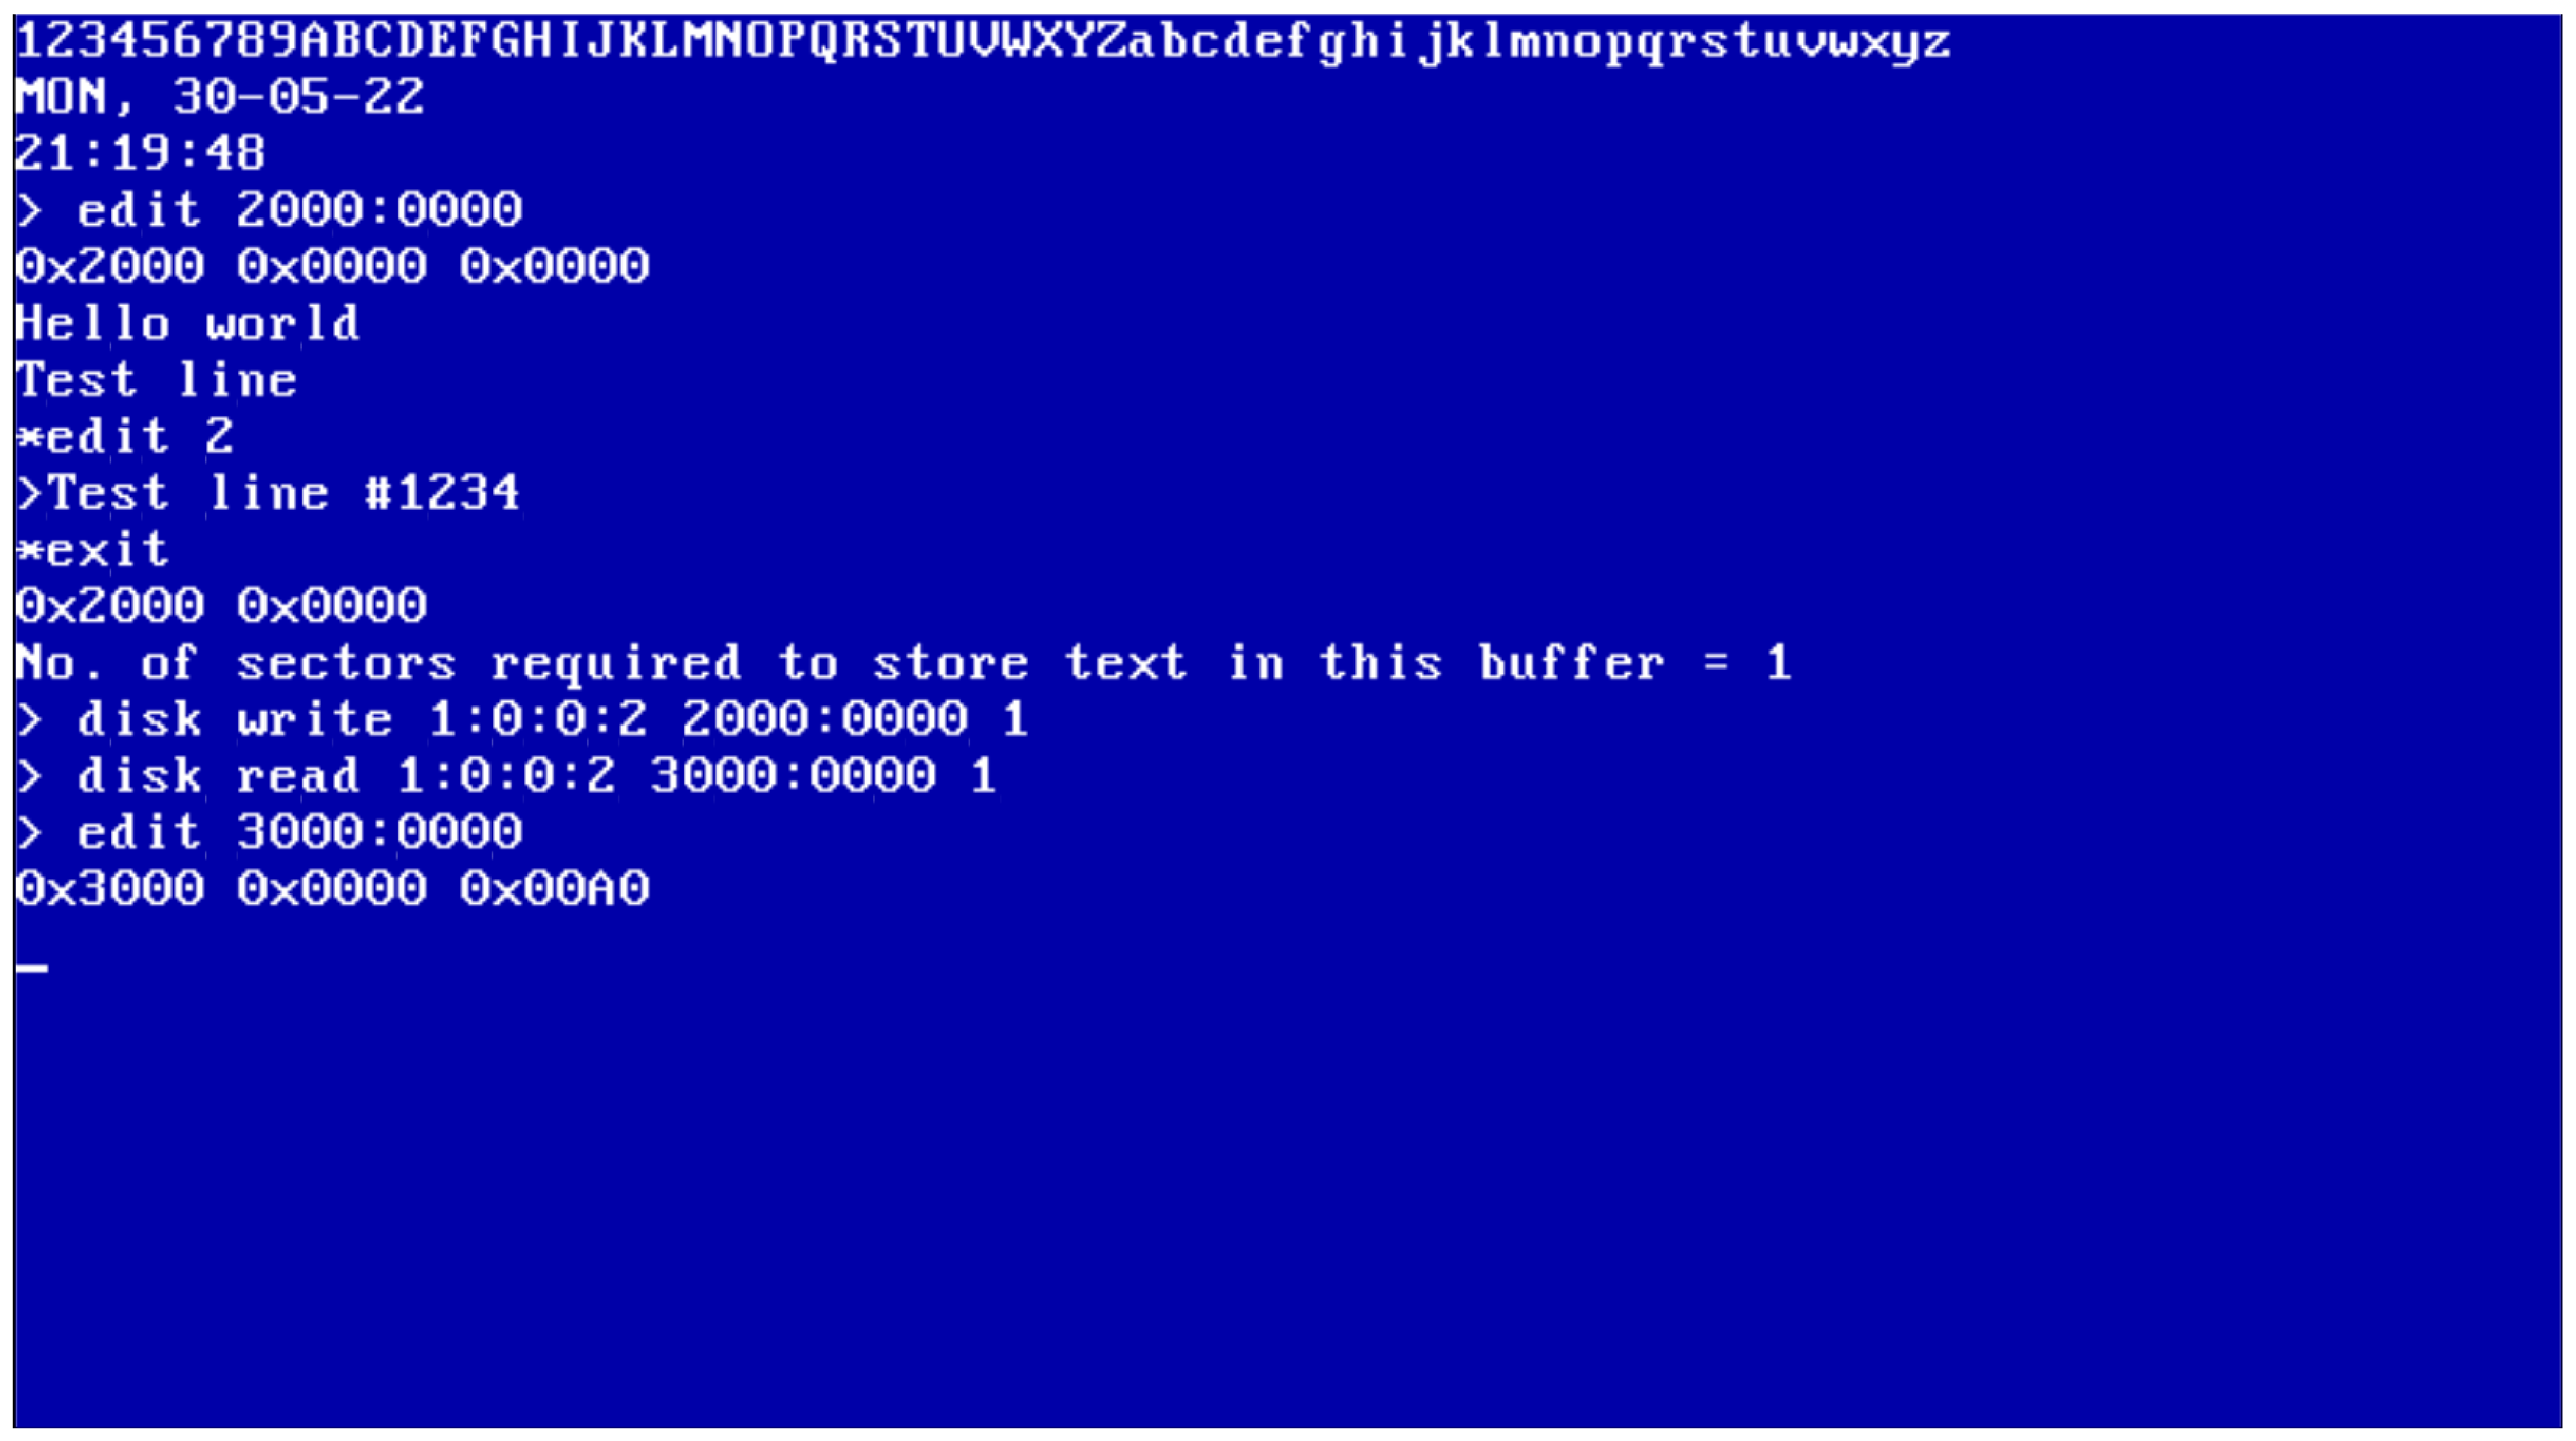
\includegraphics[scale=0.13]{figures/editor1.eps}
  \caption{Saving a new file to disk}
  \label{fig:editor1}
  \end{subfigure}
  \begin{subfigure}{.5\textwidth}
  \centering
  
\includegraphics[scale=0.13]{figures/editor2.eps}
  \caption{Successful operation of \texttt{edit} and \texttt{disk}}
  \label{fig:editor2}  
  \end{subfigure}
\caption{Using \texttt{edit} to create and edit a file}
\end{figure}

\section{Bugs}
The project has only three known bugs which is astonishing because it has been completely written in assembly language. These bugs are:
\begin{enumerate}
  \item \texttt{power level} command is not able to show the charge in the battery of the machine on which the emulator is running. This is shown in \autoref{fig:powercom}.
  \item Executing an invalid command string in the line editor insert that command string except for the asterisk. This is shown in \autoref{fig:faultycomm}.
  \item System might become unstable if an intersegment call is performed.
\end{enumerate}
\begin{figure}[H]
  \begin{subfigure}{.5\textwidth}
  \centering
  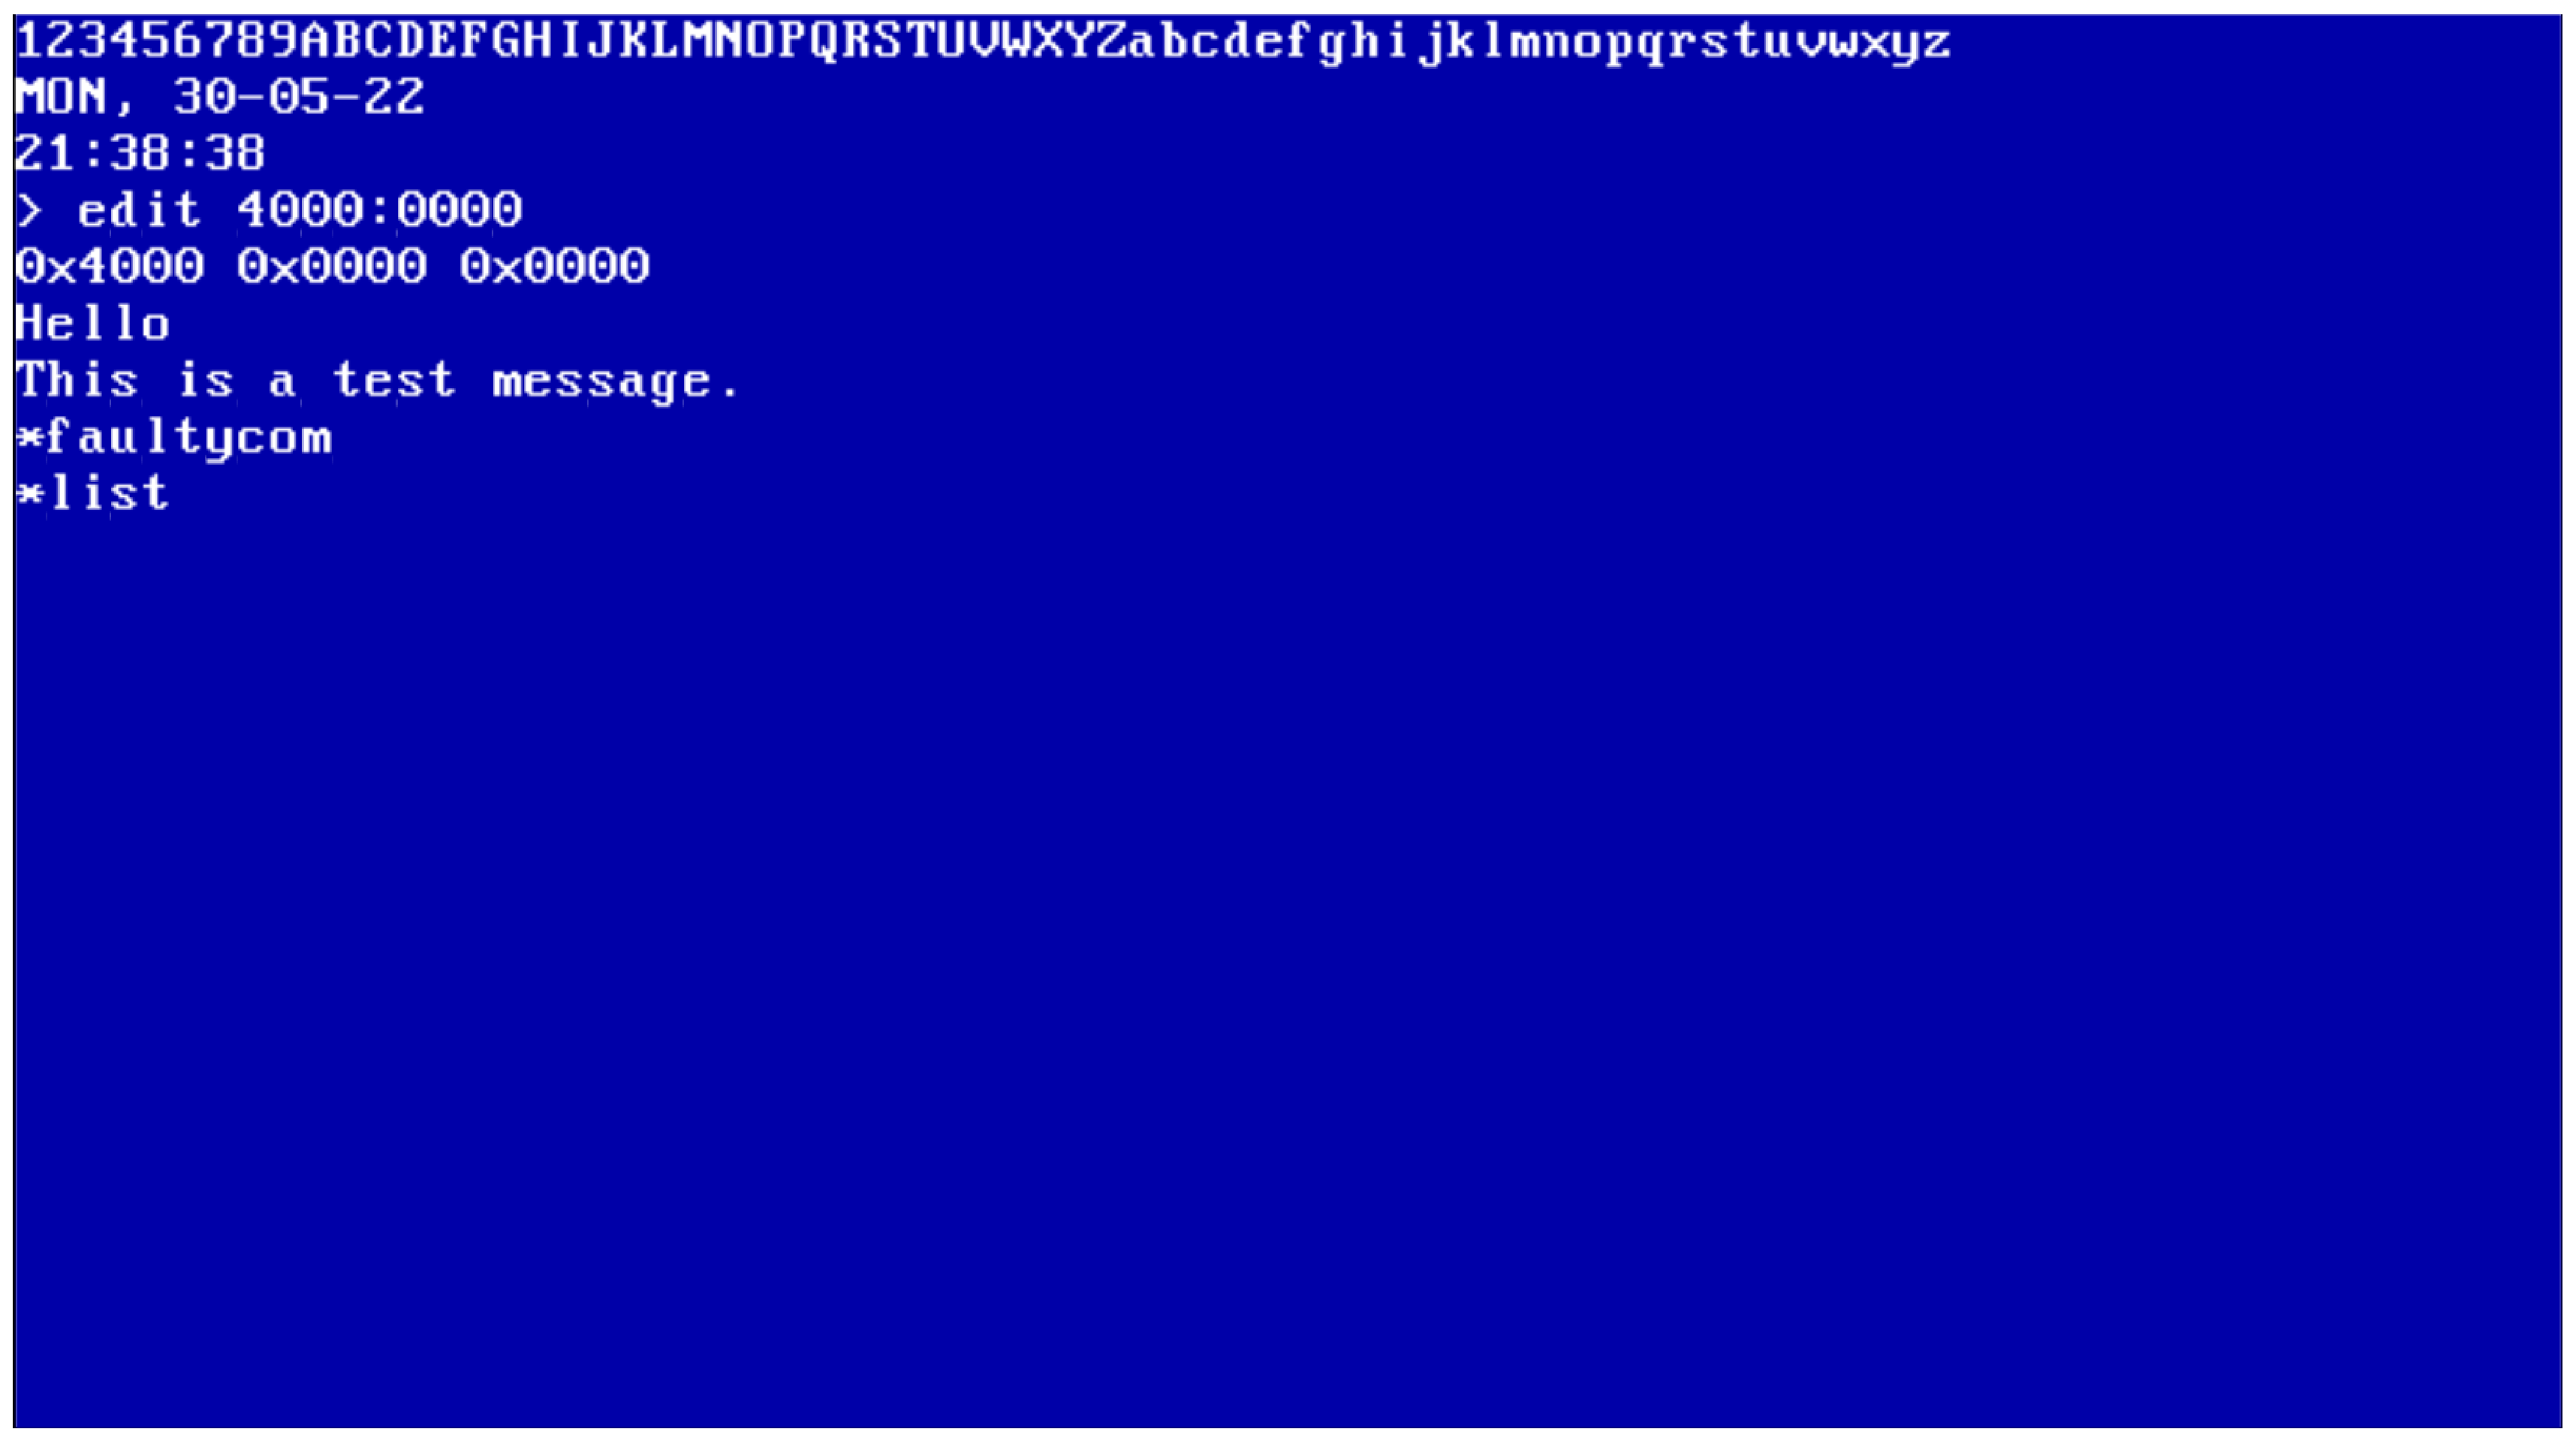
\includegraphics[scale=0.13]{figures/faultycomm1.eps}
  \caption{Entering an invalid command in the editor}
  \label{fig:faultycomm1}
  \end{subfigure}
  \begin{subfigure}{.5\textwidth}
  \centering
  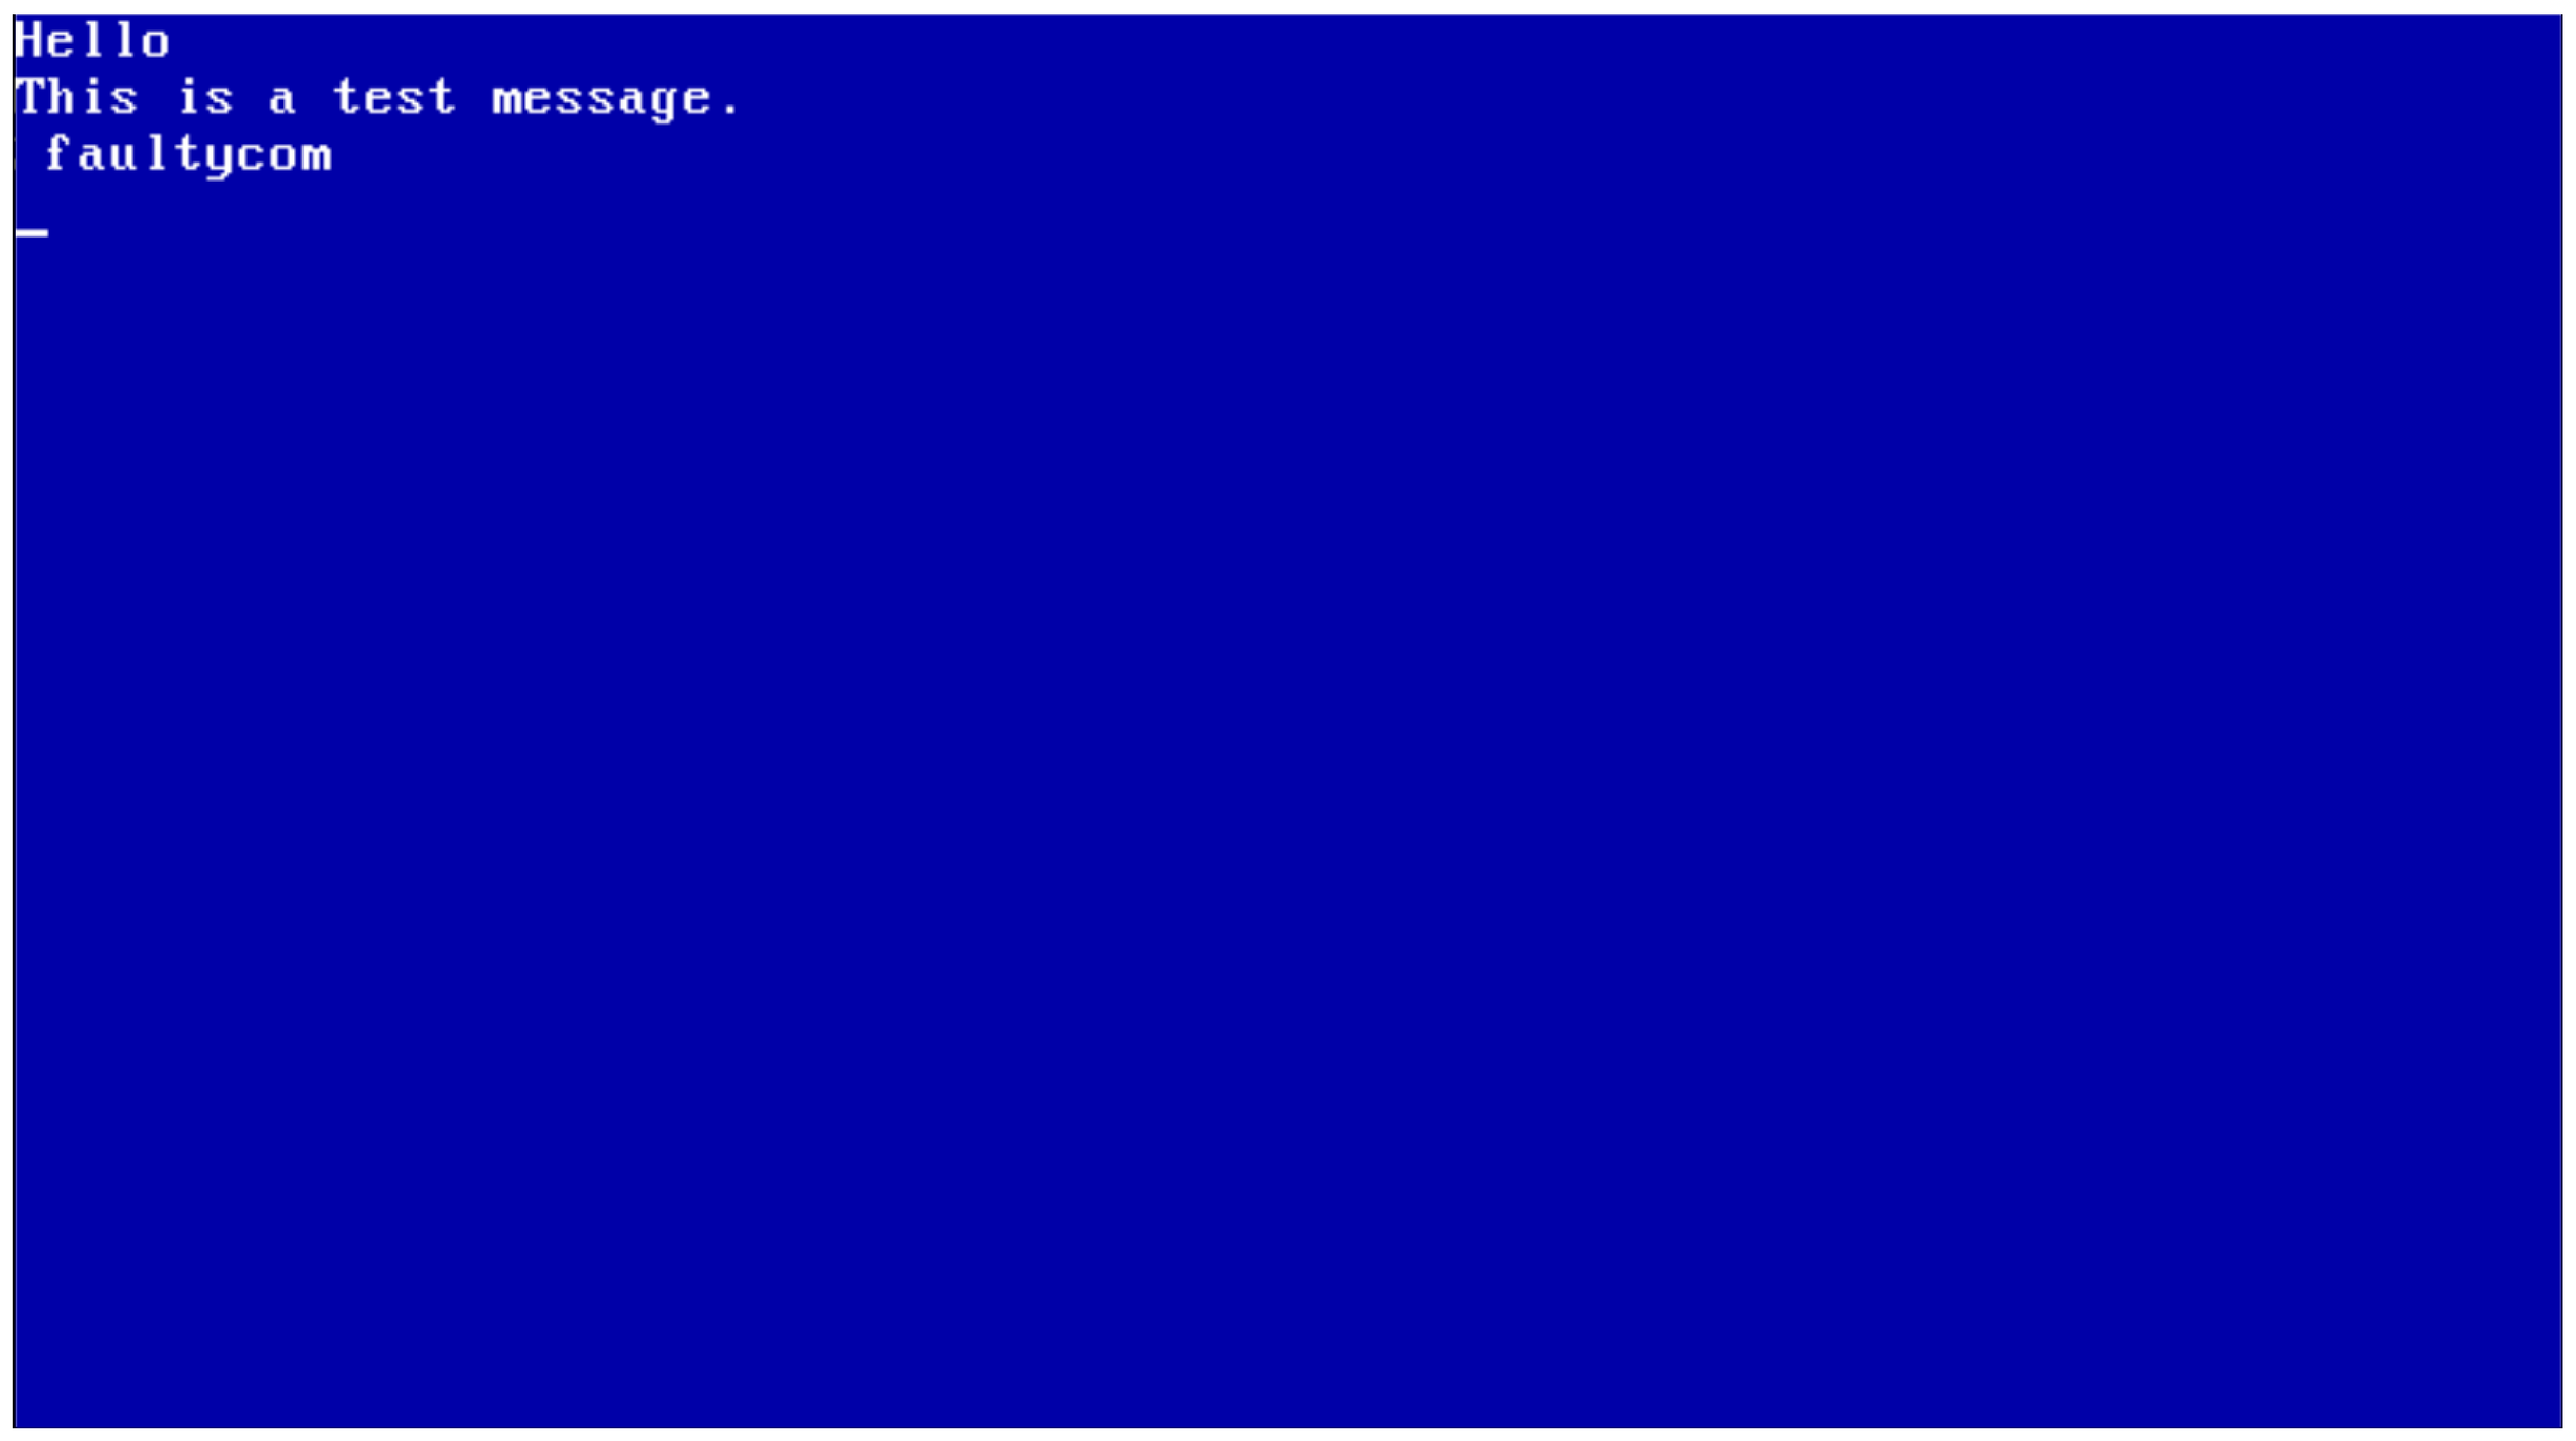
\includegraphics[scale=0.13]{figures/faultycomm2.eps}
  \caption{Listing of the file reveals the bug}
  \label{fig:faultycomm2}  
  \end{subfigure}
\caption{Bug in line editor causing it include contents of invalid commands}
\label{fig:faultycomm}
\end{figure}

\section{Discussion}
CrazyOS is comparable to disk operating systems (DOS) like CP/M and MS-DOS v1.25. Both MS-DOS v1.25 and CrazyOS have many similarities, few of which are:
\begin{enumerate}
  \item Both operating systems work in real mode.
  \item The command-prompt/shell of both of these operating system has commands built into the source code of the shell itself.
  \item Both operating systems make use of BIOS calls to access the hardware.
  \item Both of these operating system are meant for a single user only.
  \item Neither CrazyOS nor MS-DOS v1.25 has the ability to multitask between different software. 
\end{enumerate}
However, unlike MS-DOS, CrazyOS
\begin{enumerate}
  \item does not have any system calls which makes it heavily dependent on the BIOS calls provided by the OEM.
  \item does not support running applications having binary size greater than 64 kiB. Returning to shell from smaller applications after an intersegment call makes the shell unstable.
  \item does not use proper file allocation table (FAT). Therefore, disk space is not utilized efficiently.
\end{enumerate}
All modern day operating systems, like Linux kernel based distros and Windows 10, are far superior than DOS. They are one of the most complex pieces of software in the world which provide programmers and everyday users with hardware support, system calls, and file systems among many other things which allow them to use the resources of the machine efficiently and get their job done. With millions of lines of codes, even tech-gurus can only master a few integral components of the operating system in their lifetime. Clearly, the simplicity of CrazyOS comes at the cost of functionality and makes it a toy operating system which can be used for educational purposes. Porting CrazyOS for x86-64 and ARM based processors while implementing a few fundamental system calls and a file system will tremendously improve its usefulness.










%%%%%%%%%%%%%%%%%%%%%%%%%%%%%%%%%%%%%%%%%%%%%%%%%%%%%%%%%%%%%%%
\newpage
\chapter{\centering Conclusion \& Future Scope}
\section{Conclusion}
We have successfully implemented a single-user, single-tasking, real-mode operating system named CrazyOS. The operating system comes with two applications: a shell and a line editor. Both of these applications have been demonstrated to work successfully. Various subroutines responsible for handling devices and for processing user commands form the library of the operating system. These library functions can be used to develop various disk applications which can then be run from the shell, as has been successfully demonstrated by running \texttt{soundnlight.asm} program.

\section{Future Scope}
The total lines of code which are there in the project directory can be computed with the help of \texttt{cloc} utility. It is revealed that there are in total 1718 lines of assembly code. If one excludes the number of lines of code in \texttt{soundnlight.asm} program, then the total lines of code for the project comes out to be 1690. Both of these numbers show that the operating system is small enough to be read, understood, used, and played by a student over the course of their undergraduate study. If it is incorporated correctly in courses related to computer architecture and x86 microprocessor family, this operating system can prove to be useful for disseminating practical knowledge of the aforementioned project.\\
The project can be further expanded in the following ways:
\begin{enumerate}
  \item As an educational exercise, versions of CrazyOS working on computers using i386, x86-64, ARM and RISC-V processors can be developed.
  \item Documentation related to each version of CrazyOS can be published online. This will help in increasing the number of people who learn from it.
  \item A separate operating system can be developed for Raspberry Pi line of single board computers (SBC). These are easily and cheaply available all around the world. When playing with a toy operating system on a cheap SBC, the user will not have to worry about bricking their main computer. Furthermore, as RPis are increasingly being used in embedded systems, a lightweight operating system will prove to be a boon for embedded systems developers.
\end{enumerate}
We would conclude this report by quoting the words of Linus Torvalds and Terry Davis: This operating system has been developed because it was a fun challenge. Unlike Linux or Windows, it is not a professional operating system. In comparison to them, it is just a dirt-bike using which the user can go on accomplishing fun little challenges of their own liking. 
%%%%%%%%%%%%%%%%%%%%%%%%%%%%%%%%%%%%%%%%%%%%%%%%%%%%%%%%%%%%%%%%%%
\newpage
\bibliographystyle{plainnat}
\setcitestyle{numbers}
\bibliography{REFERENCES}
%%%%%%%%%%%%%%%%%%%%%%%%%%%%%%%%%%%%%%%%%%%%%%%%%%%%%%%%%%%%%%%%%%
\newpage
\chapter*{Research Paper}
\addcontentsline{toc}{chapter}{Research Paper}
\newpage
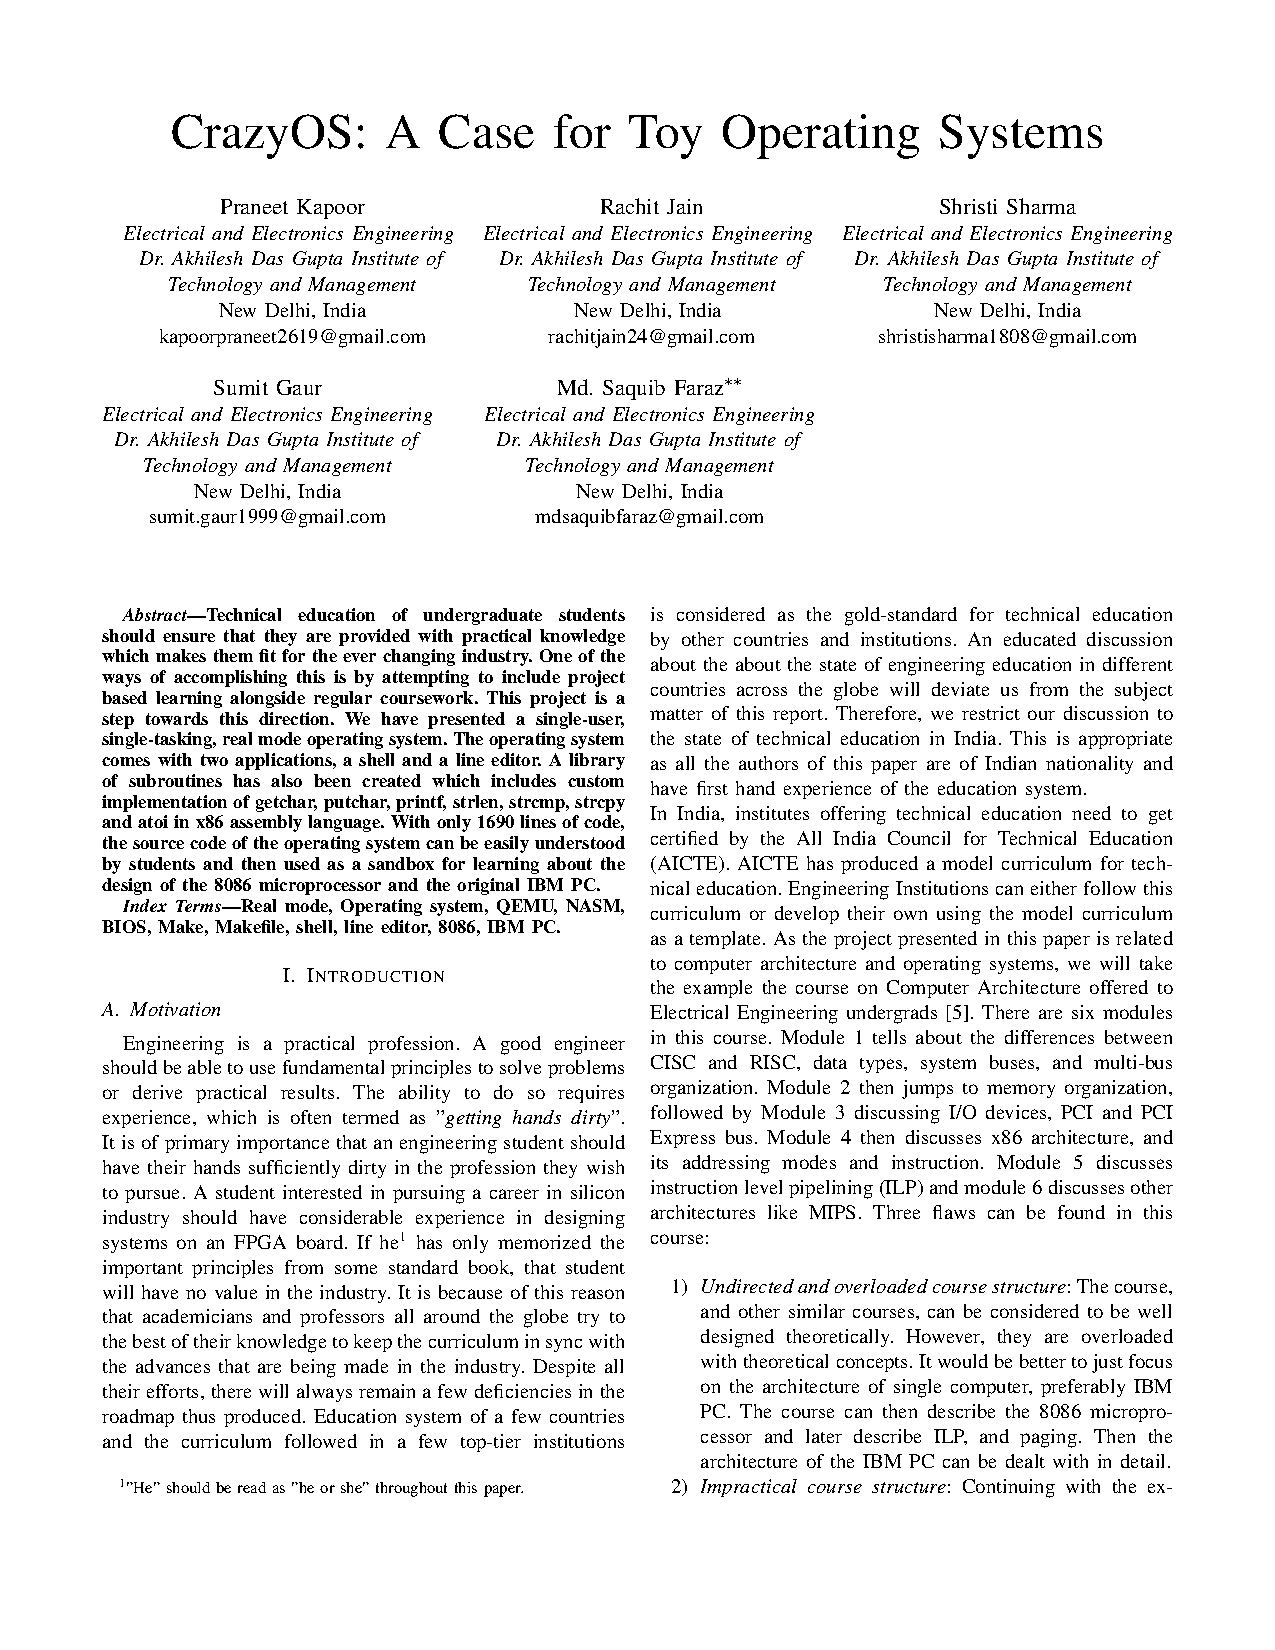
\includepdf[pages={-}]{ResearchPaper.pdf}
%%%%%%%%%%%%%%%%%%%%%%%%%%%%%%%%%%%%%%%%%%%%%%%%%%%%%%%%%%%%%%%
\newpage
\chapter*{Curriculum Vitae}
\addcontentsline{toc}{chapter}{Curriculum Vitae}
\newpage
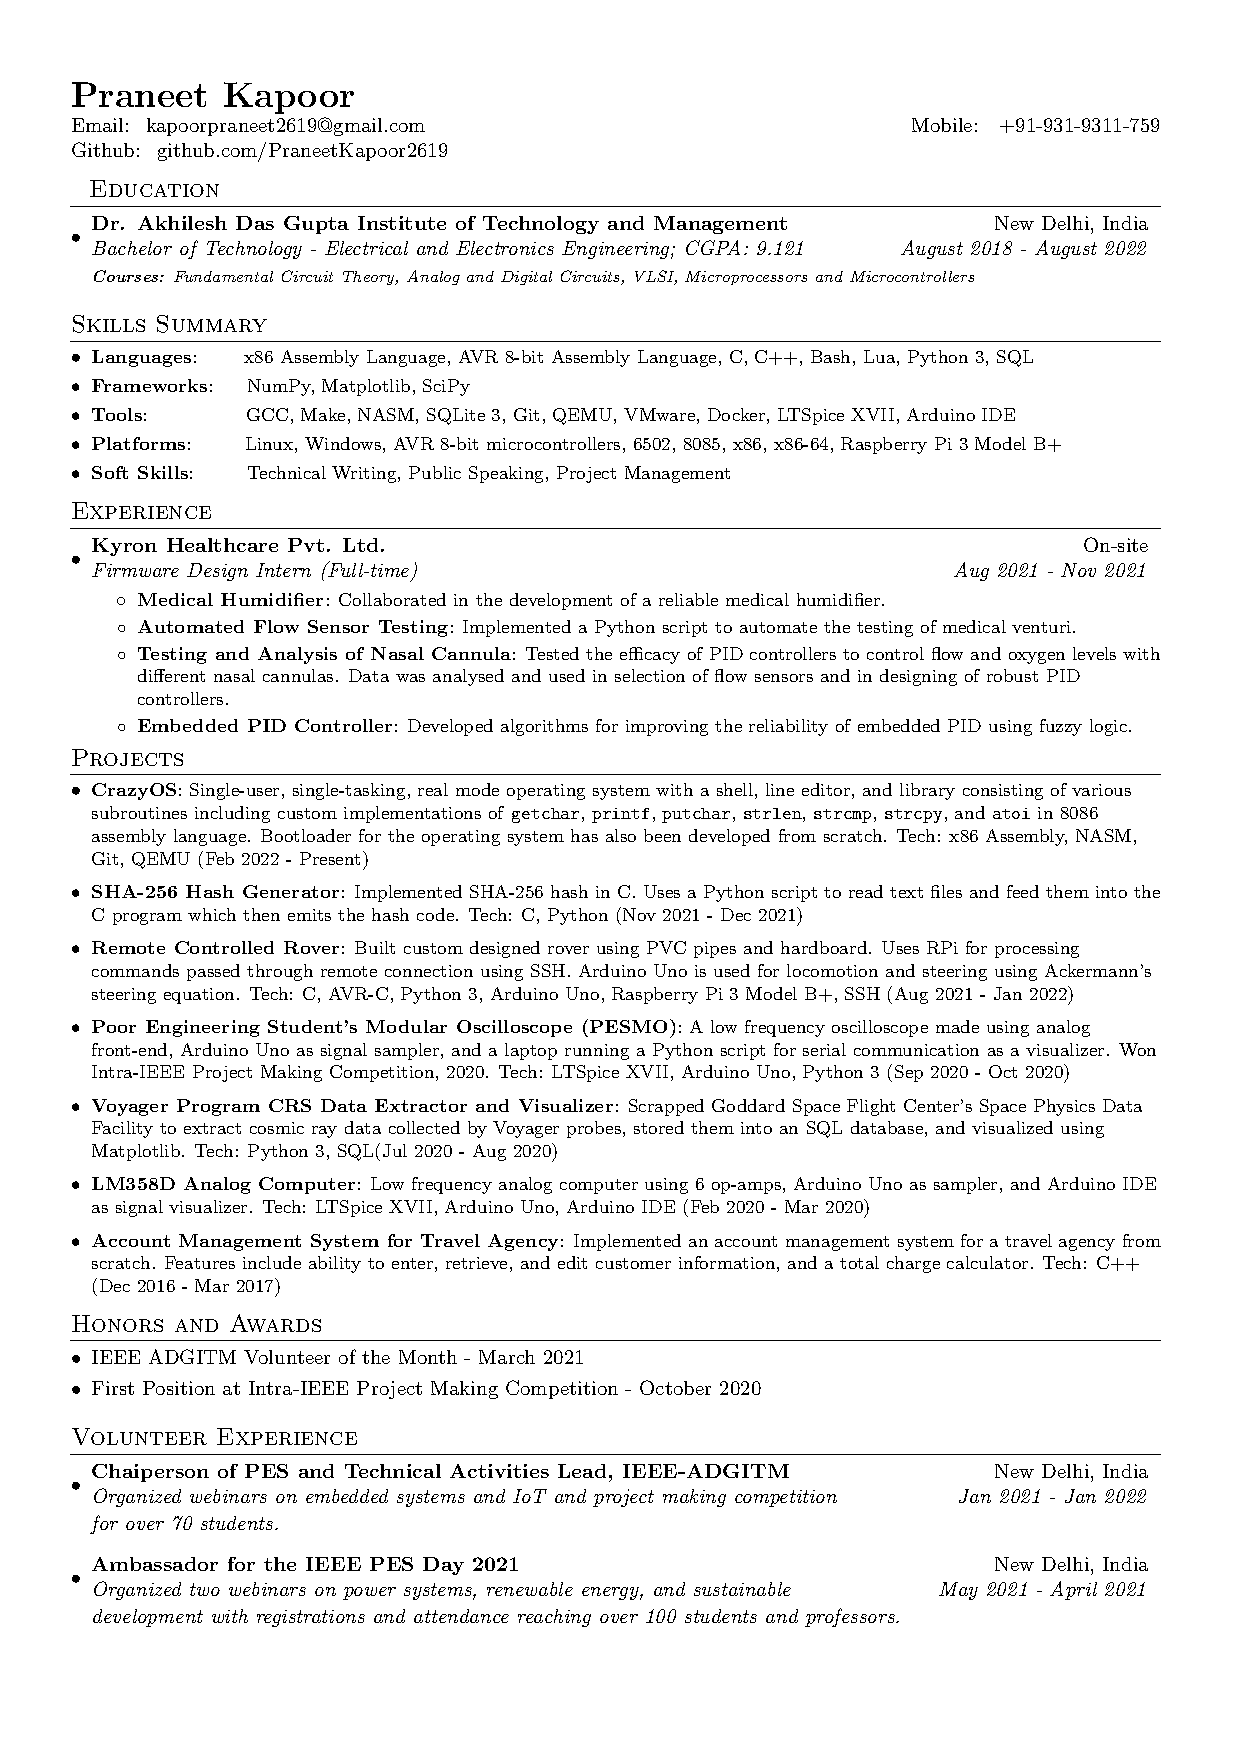
\includepdf[pages={1}]{praneet.pdf}
\newpage
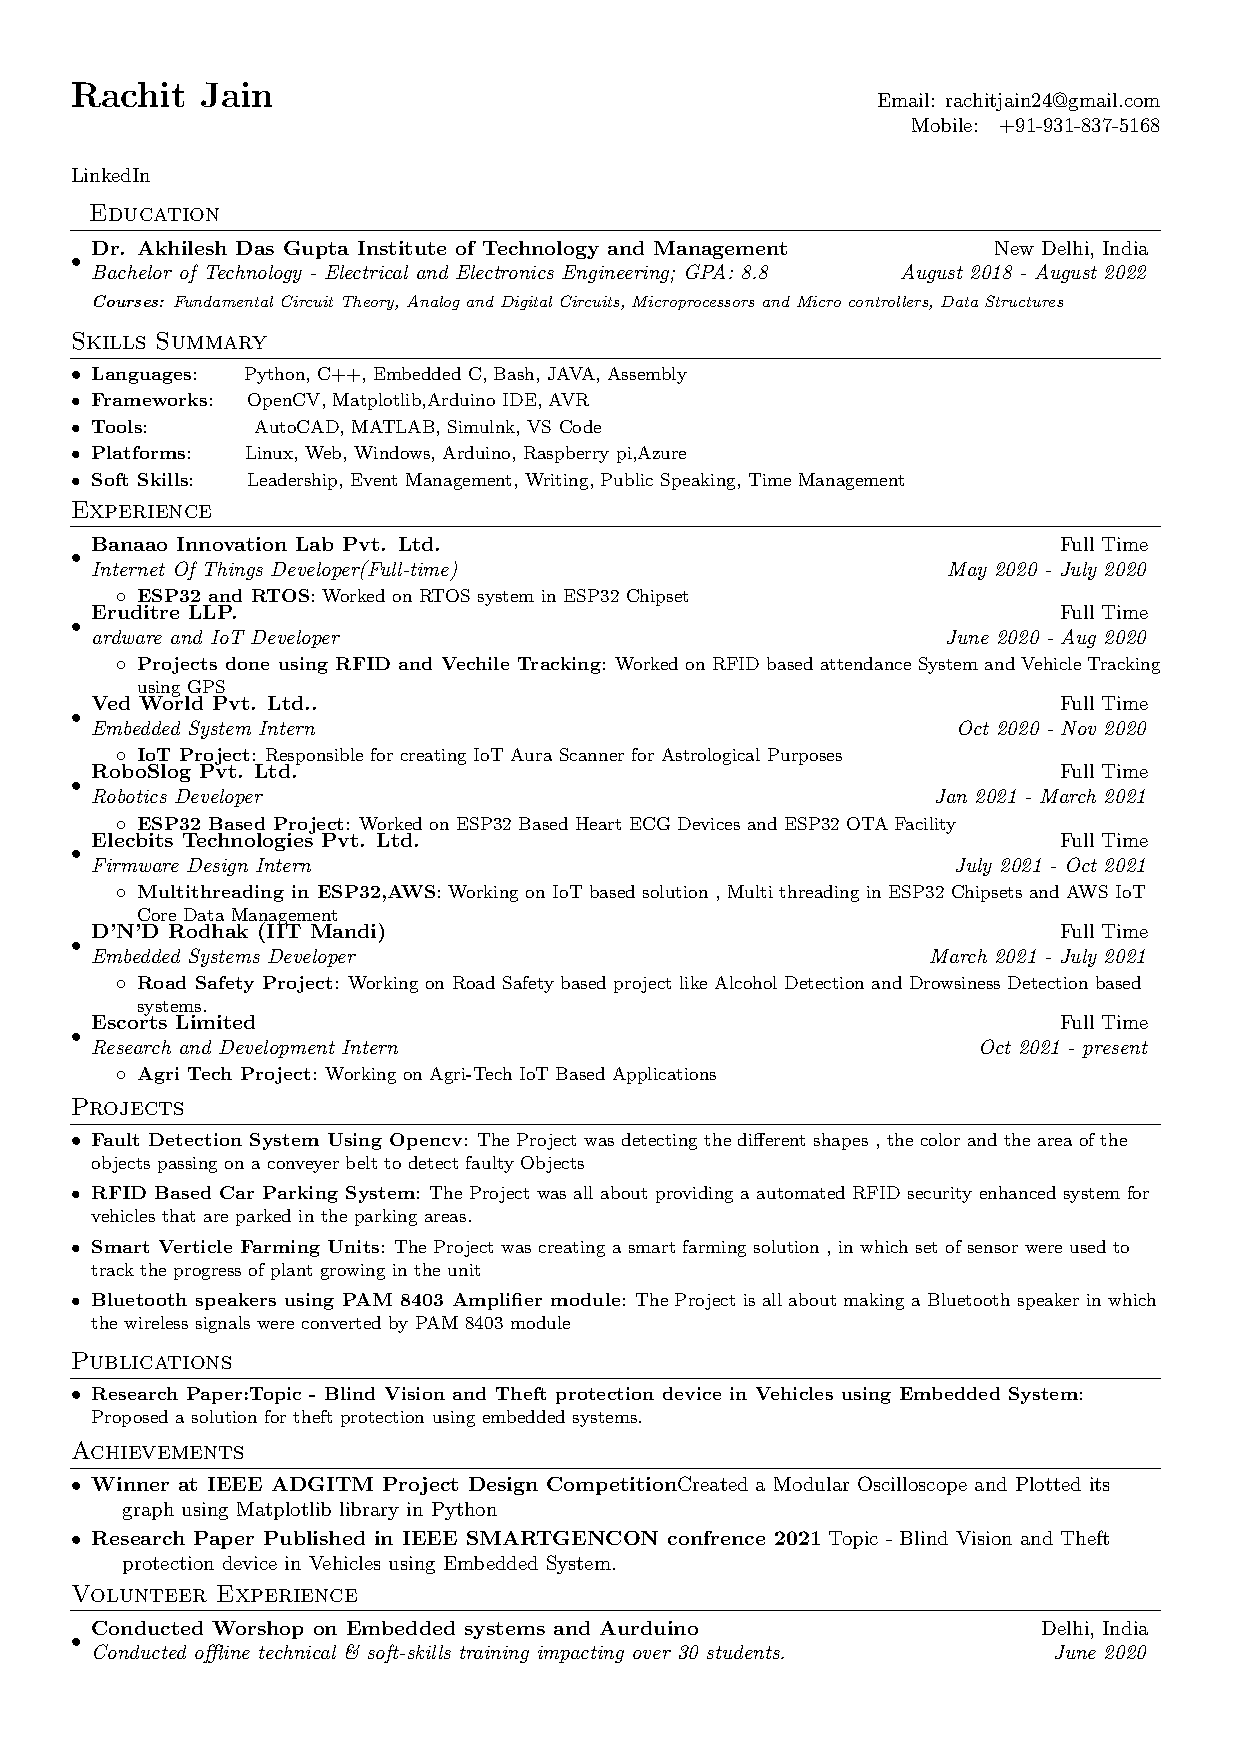
\includepdf[pages={1}]{rachit.pdf}
\newpage
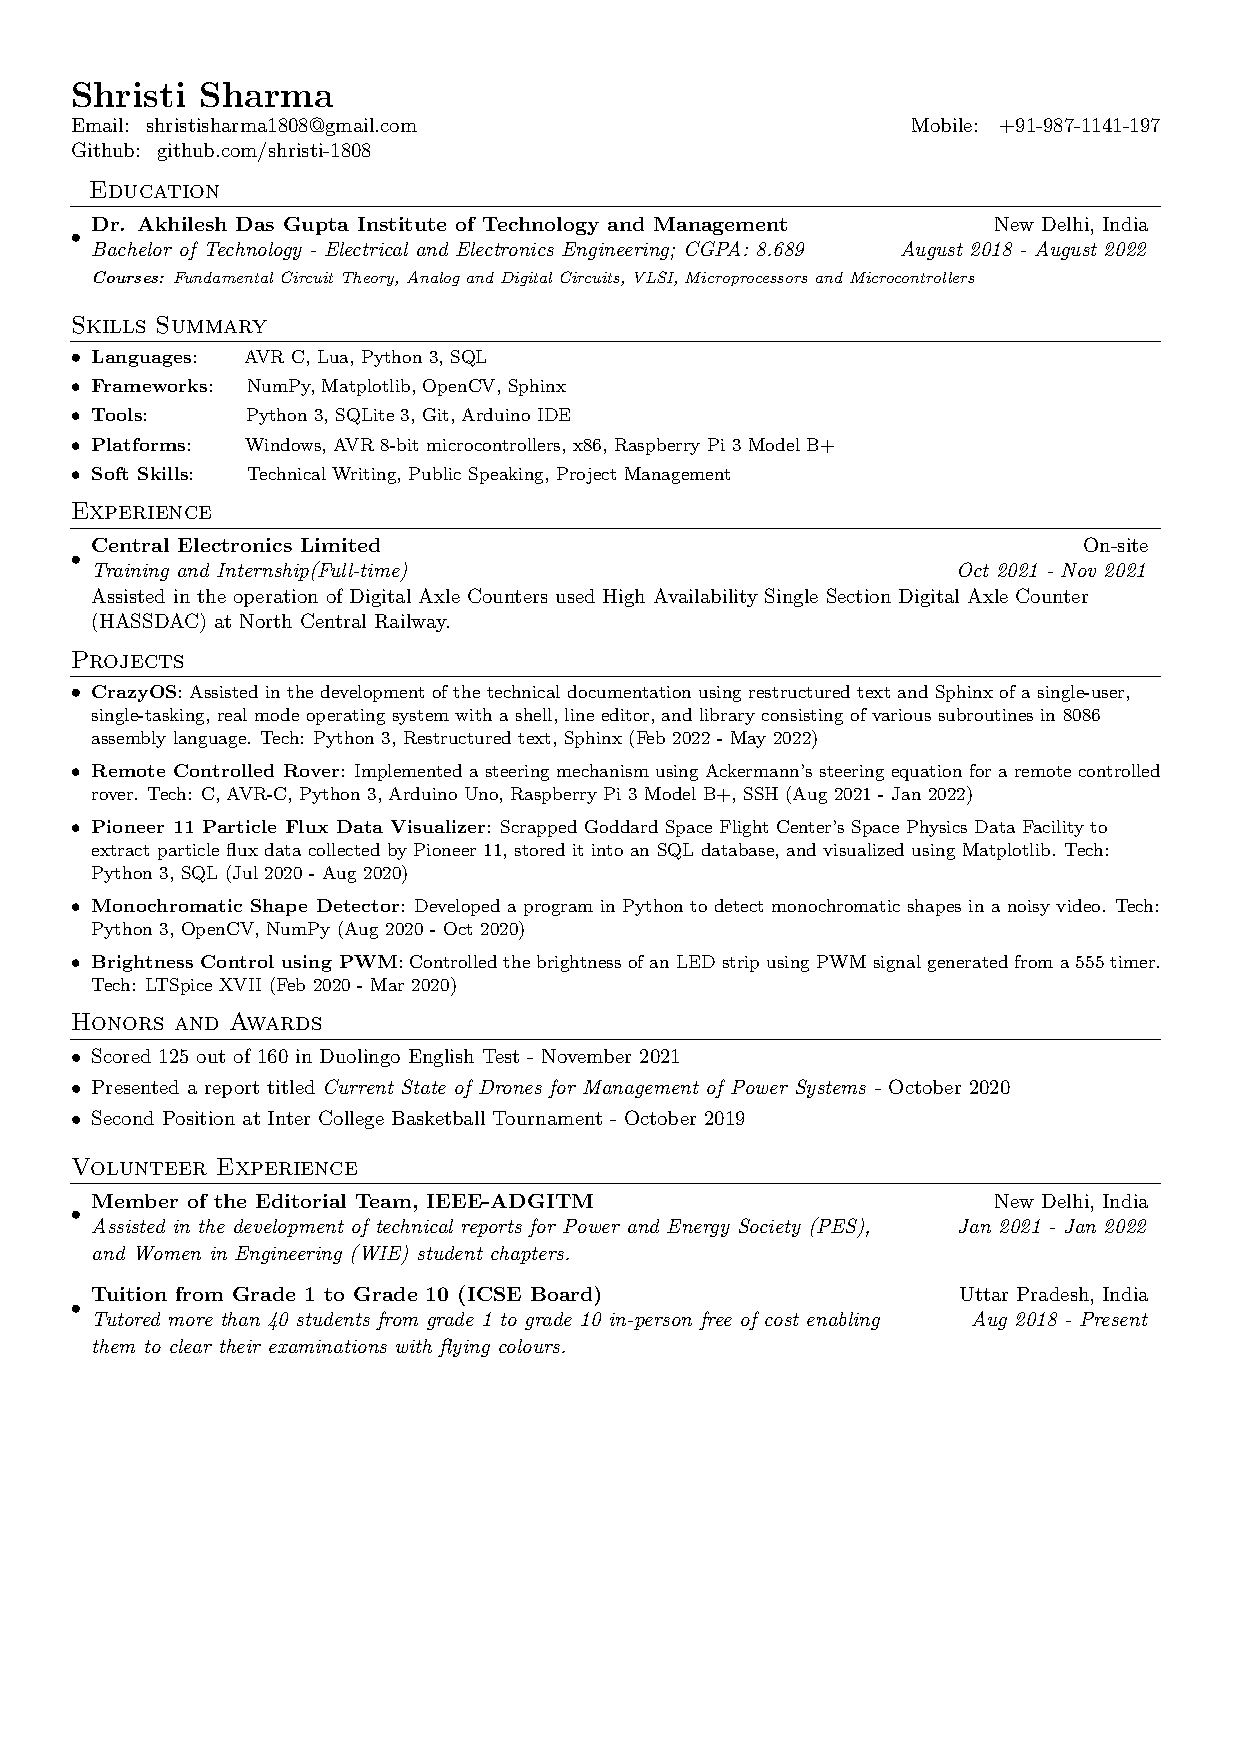
\includepdf[pages={1}]{shristi.pdf}
\newpage
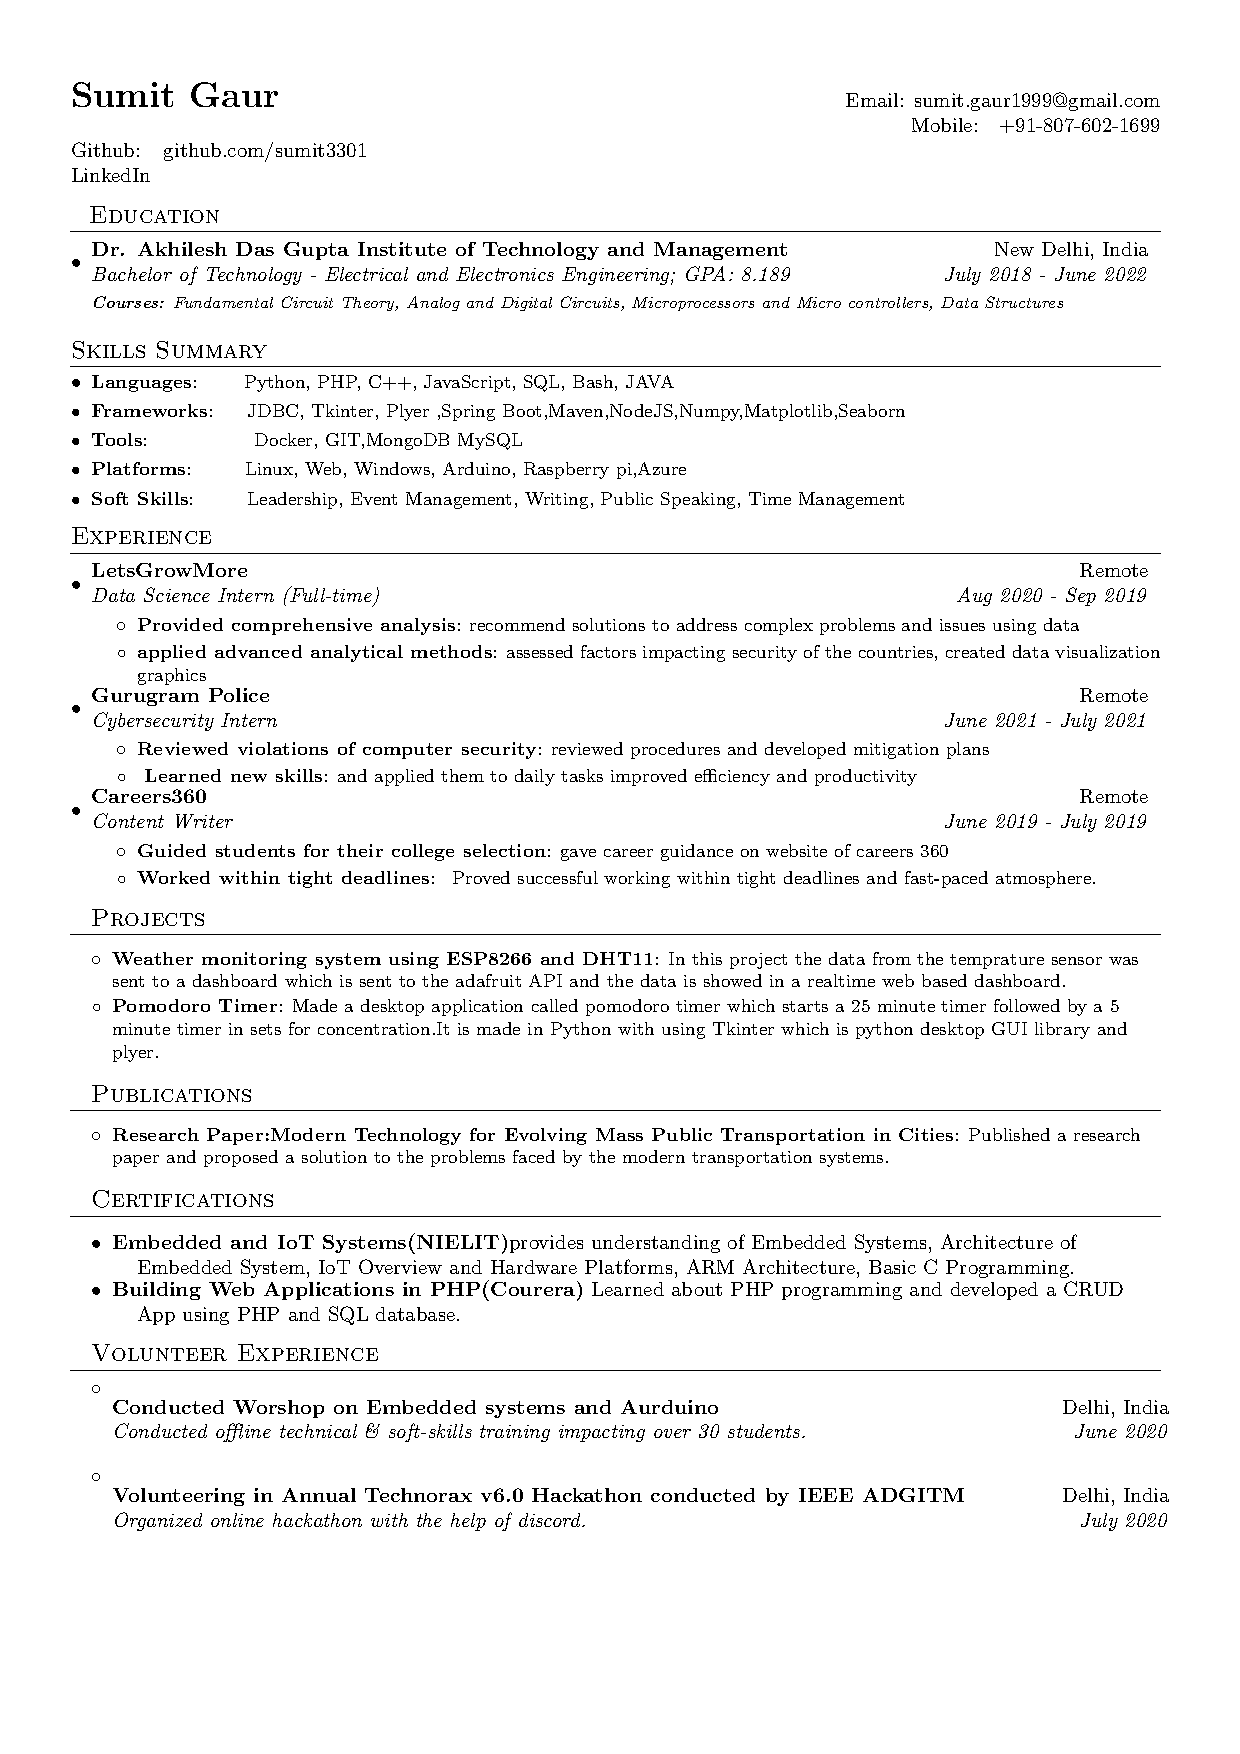
\includepdf[pages={1}]{sumit.pdf}
\newpage
%%%%%%%%%%%%%%%%%%%%%%%%%%%%%%%%%%%%%%%%%%%%%%%%%%%%%%%%%%%%%%%
\end{document}